\documentclass{ut-thesis}

%**************************** General libraries *******************************
\usepackage{mathtools}
\usepackage{cancel}
\usepackage[utf8]{inputenc} 
\usepackage{amssymb}
\usepackage{ntheorem}
\usepackage{tensor}
%\usepackage{physics}
\usepackage[italicdiff]{physics}
\usepackage{calc}
\usepackage{caption}
%\usepackage{subcaption}
\usepackage{tcolorbox}
\usepackage{chngcntr}
\usepackage{titlesec}
\usepackage {graphicx,float} 
\usepackage{subfig}
\usepackage{siunitx}
\usepackage{xcolor}
\usepackage{etoolbox} %ifthen
\usepackage[outline]{contour} % glow around text

%**************************** Bibliography management *******************************
\usepackage{biblatex} %Imports biblatex package
\addbibresource{sample.bib} %Import the bibliography file



%**************************** Tikz libraries *******************************
\usepackage{tikz}
\usetikzlibrary{shapes,arrows,arrows.meta,spy}
\usetikzlibrary{calc}% needed for BB
\usepackage{pgfplots}
\usetikzlibrary{math} % for \tikzmath
\usetikzlibrary{angles,quotes} % for pic (angle labels)
\usetikzlibrary{decorations.pathmorphing,decorations.markings}
\usetikzlibrary{decorations.pathreplacing} % for curly braces
\usetikzlibrary {decorations.markings,shapes.arrows}
\usetikzlibrary{patterns}
\usepackage{tkz-euclide}
\usepackage{tikz-3dplot}

%\usepackage[margin=0cm,nohead]{geometry}
%\usepackage[active,tightpage]{preview}
%\usepackage[pdf]{pstricks}

%**************************** custom macro's *******************************
\newsavebox\CBox
\newcommand\hcancel[2][0.5pt]{%
  \ifmmode\sbox\CBox{$#2$}\else\sbox\CBox{#2}\fi%
  \makebox[0pt][l]{\usebox\CBox}%  
  \rule[0.5\ht\CBox-#1/2]{\wd\CBox}{#1}}
%\newcommand{\edal}{\end{align}}
%\newcommand{\bgal}{\begin{align}\end{align}}
\newcommand{\Lagr}{\mathcal{L}}
\newcommand{\questeq}{\overset{?}{=}}
%\newtheorem{theorem}{Theorem}
\newtheorem{lemma}{Lemma}
\renewcommand\thelemma{\unskip}
\newcommand{\christ}[3]{\ensuremath{\Gamma^{#1}_{#2#3}}}
\newcommand{\half}{\ensuremath{\frac{1}{2}}}
\newcommand{\kwart}{\ensuremath{\frac{1}{4}}}
\newcommand\del{\overline{\boldsymbol{{\triangledown}}}}
\newcommand\maal{\boldsymbol{\times}}
\newcommand\spatie{\quad\quad\quad\quad}
\newcommand\RAr{\quad\Rightarrow\quad}
%\newcommand{\myabsdv}[3]{{\frac{\delta^2 \ensuremath{{#1}}}{{\delta %%\ensuremath{{#2}}}{\delta\ensuremath{{#3}}}}}}
\newcommand\myabsdv[3][1]{{\frac{{\delta^{2}}{#1}}{\delta {#2} \delta {#3}}}}

%**************************** layout setings *******************************
\counterwithin*{equation}{chapter}
\counterwithin*{equation}{section}
\counterwithin*{equation}{subsection}
\renewcommand{\theequation}{\arabic{equation}}
\titleformat{\chapter}{\normalfont\huge}{\thechapter.}{20pt}{\huge\it}
\titleformat{\chapter}[display]
  {\normalfont\bfseries}{}{0pt}{\Huge}
\titlespacing*{\chapter}{0pt}{50pt}{*2}
\newcommand{\RomanNumeralCaps}[1]{\MakeUppercase{\romannumeral #1}}

%**************************** Tikz  setings *******************************
\begin{comment}
\tikzset{
    circ/.style={draw, circle,inner sep=0pt,minimum size=8mm, font=\scriptsize},
    triangle/.tip={Computer Modern Rightarrow[open,angle=120:3pt]}}
    
\tikzset{
  every point/.style = {circle, inner sep={.75\pgflinewidth}, opacity=1, draw, solid, fill=white},
  point/.style={insert path={node[every point, #1]{}}}, point/.default={},
  colored point/.style = {point={fill=#1}},
  point name/.style = {insert path={coordinate (#1)}},
  inherit/.style = {point/.style={insert path={node[circle, inner sep={.75\pgflinewidth}, draw, fill, #1]{}}}}
}
\end{comment}

%**************************** Where to find images *****************************
%\graphicspath{ {images/} }
%\graphicspath{ {./images/} }


%**************************** Document itself *******************************
\author{Bernard Carrette}
%\gradyear{1979}
\title{Tensor Calculus\\J.L. Synge and A.Schild (Dover Publication)\\ Solutions to exercises\\Part II\\
Chapters \RomanNumeralCaps{5} to \RomanNumeralCaps{8}}
\begin{document}
\maketitle

\tableofcontents
\listoffigures
%\setcounter{chapter}{4}
\chapter{Applications to Classical Mechanics}
\pagebreak[4]
\section{p153 - Exercise}
\begin{tcolorbox}
If $\mu^{\alpha}$ are the contravariant components of a unit vector in a surface $S$, show that $\mu^{\alpha}f_{\alpha}$ is the physical component of acceleration in the direction tangent to $S$ defined by $\mu^{\alpha}$.
\end{tcolorbox}
As we are in an Euclidean space we can interpret $a_{mn}\mu^{\alpha}f^{\alpha}$ as $\left|\mu\right|\left|f\right|\cos\theta $ with $\theta$ the angle between the two vectors. As $\left|\mu\right|=1$ we have
\begin{align}
a_{mn}\mu^{\alpha}f^{\alpha}&= \mu^{\alpha}f_{\alpha}\\
&= \left|f\right|\cos\theta 
\end{align}
which is the projection of the vector $f$ on the unit vector $\mu$.
$$\blacklozenge$$
\newpage

\section{p154 - Clarification to 5.226.}
\begin{tcolorbox}
$$\mathbf{\text{5.226.}\spatie v\dv{v}{s}=0,\quad \overline{\kappa}v^2=0}$$
Assuming that the particle is not at rest $v\ne 0$, and therefore $\overline{\kappa}=0$. \textit{\textbf{Since this implies that the curve is a geodesic}...}
\end{tcolorbox}
The assertion in bold is a direct consequence $$\mathbf{\text{2.513.}}\spatie \frac{\delta \dv{x^r}{s}}{\delta s}=0$$ 
As in $ \mathbf{5.233}$ we have $\frac{\delta \lambda^{\alpha}}{\delta s}=\frac{\delta \dv{x^{\alpha}}{s}}{\delta s}=0$, the considered curve follows the geodesic curve.
$$\blacklozenge$$
\newpage

\section{p155 - Exercise}
\begin{tcolorbox}
Show that in relativity the force $4$-vector $X^r$ lies along the first normal of the trajectory in space-time. Express the first curvature in terms of the proper mass $m$ of the particle and the magnitude $X$ of $ X^r$.
\end{tcolorbox}
Let us recall the first Frenet formula $\mathbf{2.705}$ without forgetting that the metric form is not positive-definite, $$\frac{\delta \lambda^r}{\delta s}=\kappa\nu^r,\quad \epsilon_{(1)}\nu_n\nu^n=1$$ As $\mathbf{5.299}$ $$m\frac{\delta \lambda^r}{\delta s}=X^r$$ it is clear that $X^r = m\kappa\nu^r$ and is collinear with the first normal.
\begin{align}
X^r &= m\kappa\nu^r\\
\times \quad a_{mr}X^m\quad\Rightarrow\spatie \underbrace{a_{mr}X^mX^r}_{=\left(X^1\right)^2+\left(X^2\right)^2+\left(X^3\right)^2-\left(X^4\right)^2} &= m\kappa \underbrace{a_{mr}\nu^m\nu^r}_{= \epsilon_{(1)}}
\end{align}
\textbf{$$\Rightarrow\spatie \kappa = \epsilon_{(1)}\frac{\left(X^1\right)^2+\left(X^2\right)^2+\left(X^3\right)^2-\left(X^4\right)^2}{m}
$$}
$$\blacklozenge$$
\newpage


\section{p156 - Clarification}
\begin{tcolorbox}
Interpretation of 
$$\mathbf{5.231.}\spatie M_{rs}=\epsilon_{rsn}M_n=z_rF_s-z_sF_r$$
\end{tcolorbox}
What do the $M_{rs}$ represent?
\begin{figure}[H]

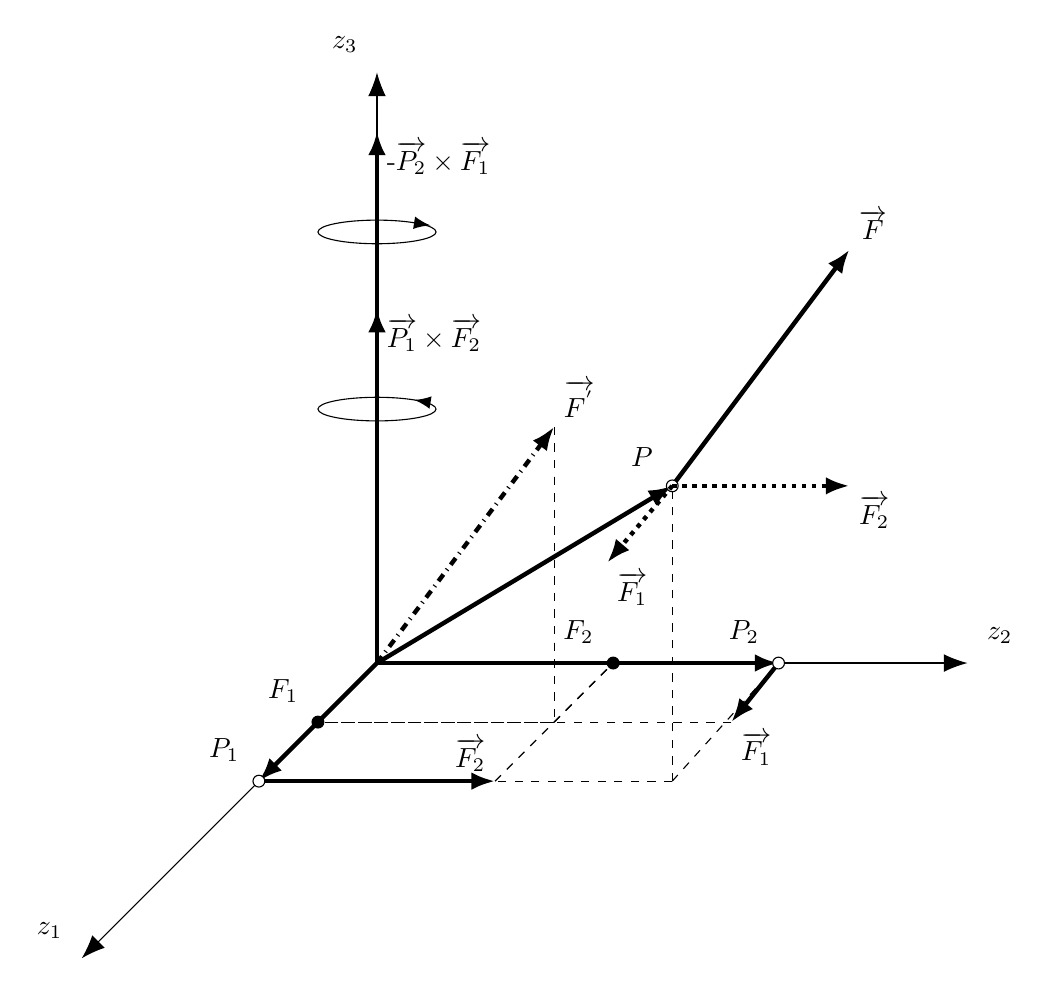
\begin{tikzpicture}[scale=0.75]
\tikzstyle{left-hand-mirror} = [
    draw,
    postaction=decorate, 
    decoration={
        markings,
        mark=between positions 0.015 and 0.98 step 0.1072 with {\draw (0,0)--(60:3pt);}
    }
]  
\coordinate (O) at (0,0);
\coordinate (X) at (-5,-5);
\coordinate (Y) at (10,0);
\coordinate (Z) at (0,10);
\draw [-{Latex[length=3mm]}] (O) -- (X);
\draw [-{Latex[length=3mm]}] (O) -- (Y);
\draw [-{Latex[length=3mm]}] (O) -- (Z);
\node[label=north west:$z_1$] at (X) {};
\node[label=north east:$z_2$] at (Y) {};
\node[label=north west:$z_3$] at (Z) {};
\coordinate (P) at (5,3);
\draw [-{Latex[length=3mm]},ultra thick] (O) -- (P);
\node[label=north west:$P$] at (P) {};
\coordinate (F) at (8,7) {};
\draw [-{Latex[length=3mm]}, ultra thick] (P) -- (F);
\node[above right] at (F) {$\overrightarrow{F}$};
\coordinate (Fp) at (8-5,7-3) {};
\draw [-{Latex[length=3mm]},dashdotted,ultra thick] (O) -- (Fp);
\node[above right,] at (Fp) {$\overrightarrow{F^{'}}$};
\coordinate (Px) at (-2,-2) {};
\coordinate (Py) at (6.8,0) {};
\node[label=north west:$P_1$] at (Px) {};
\node[label=north west:$P_2$] at (Py) {};
\coordinate (Pp) at (5,-2) {};
\draw [dashed] (Pp) -- (P);
\draw [dashed] (Pp) -- (Px);
\draw [dashed] (Pp) -- (Py);
\coordinate (Fpp) at (3,-1) {};
\coordinate (Fx) at (-1,-1) {} {};
\coordinate (Fy) at (4,0) {} {};
\node[label=north west:$F_1$] at (Fx) {};
\node[label=north west:$F_2$] at (Fy) {};
\draw[fill = black]  (Fx) circle (0.1);
\draw[fill = black]  (Fy) circle (0.1);
\draw [dashed] (Fp) -- (Fpp);
\draw [dashed] (Fpp) -- (Fx);
\draw [dashed] (Fpp) -- (Fy);

\coordinate (Fppp) at (6,-1) {} {};
\coordinate (Pppp) at (2,-2) {} {} {};
\node[{anchor=north west }] at (Fppp) {$\overrightarrow{F_1}$};
\node[{anchor=south east }] at (Pppp) {$\overrightarrow{F_2}$};
\draw [-{Latex[length=3mm]}, ultra thick] (O) -- (Px);
\draw [-{Latex[length=3mm]},ultra thick] (O) -- (Py);
\draw [-{Latex[length=3mm]}, ultra thick] (Px) -- (Pppp);
\draw [-{Latex[length=3mm]},ultra thick] (Py) -- (Fppp);
%\node[label=north west:$K$] at (Fppp) {};
%\node[label=north west:$S$] at (Pppp) {};
\draw [dashed] (Fp) -- (Fpp);
\draw [dashed] (Fppp) -- (Fx);
\draw [dashed] (Pppp) -- (Fy);
%\filldraw[ultra thick, gray!10] (Px) -- (Pppp) -- (Fy) -- (O) -- (Px) -- cycle;
%\filldraw[ultra thick,gray!20] (Fx) -- (Fppp) -- (Py) -- (O) -- (Px) -- cycle;
%\draw[ultra thick, gray!80] (Px) -- (Pppp) -- (Fy) -- (O) -- (Px) -- cycle;
%\draw[ultra thick,gray!80] (Fx) -- (Fppp) -- (Py) -- (O) -- (Px) -- cycle;
\coordinate (Vp1) at (0,6) {} {};
\coordinate (Vp2) at (0,9) {} {} {};
\draw [-{Latex[length=3mm]}, ultra thick] (O) -- (Vp1);
\draw [-{Latex[length=3mm]}, ultra thick] (O) -- (Vp2);
\node[{anchor=north west }] at (Vp1) {$\overrightarrow{P_1}\times\overrightarrow{F_2}$};
\node[{anchor=north west }] at (Vp2) {-$\overrightarrow{P_2}\times\overrightarrow{F_1}$};
\draw[fill=white]  (Py) circle (0.1);
\draw[fill=white]  (Px) circle (0.1);
\draw[fill=white]  (P) circle (0.1);
\draw[decoration={markings, mark=at position 0.1 with {\arrow[scale = 1.5]{latex[]}}},
    postaction={decorate}](0,4.3) ellipse (1 and 0.2);
    \draw[decoration={markings, mark=at position 0.1 with {\arrow[scale = 1.5]{latex[reversed]}}},
    postaction={decorate}](0,7.3) ellipse (1 and 0.2);
 \coordinate (Qx) at (3.9,1.7) {} {};
\coordinate (Qy) at (8,3) {} {} {};
\draw [-{Latex[length=3mm]},dotted, ultra thick] (P) -- (Qx);
\draw [-{Latex[length=3mm]},dotted, ultra thick] (P) -- (Qy);
\node[{anchor=north west }] at (Qx) {$\overrightarrow{F_1}$};
\node[{anchor=north west }] at (Qy) {$\overrightarrow{F_2}$};
\end{tikzpicture}
\caption{Interpretation of the tensor moment $M_{12}$}
\label{fig:fig_p156_5320}
\end{figure}
Let's consider a mass point $P$ on which a force $\overrightarrow{F}$ is acting. The force has components $\left(F_x,F_y,F_z\right)$ in the  space $V^{'}_3$ (which is by the way not the space $V_3$ of the considered mass point).\\
Let's investigate the element $M_{12}$ of the \textit{tensor moment}.\\
$P_1F_2\overrightarrow{e_3}$ is the vector product $\overrightarrow{P_1}\times\overrightarrow{F_2}$ and is as such the torque of the component $F_2$ of $\overrightarrow{F}$ acting on the mass point situated at $P_1$. The origin being fixed, $\overrightarrow{F_2}$ tries to move $P_1$, clockwise along the $z_3$ axis. The same is true for the component $\overrightarrow{F_1}$ acting on the mass point situated at $P_2$, and is represented here by the vector $- \overrightarrow{P_2}\times\overrightarrow{F_1}$ ($\overrightarrow{F_1}$ tries to move  $P_2$, counter clockwise along the $z_3$ axis). \\
Hence, $P_1F_2-P_2F_1$ is the net force trying to move the point $P$ along the $z_3$ axis (i.e. in the plane $\parallel$ with the $z_3=0$ plane).
$$\blacklozenge$$
\newpage


\section{p156 - Clarification}
\begin{tcolorbox}
$$\mathbf{5.234.}\spatie \dv{h_r}{t}= M_r$$
\end{tcolorbox}
\begin{align}
h_r &= m\epsilon_{rmn}z_mv_n\\
\Rightarrow \spatie \dv{h_r}{t} &= m\epsilon_{rmn}\dv{z_m}{t} v_n+m\epsilon_{rmn}z_m\dv{v_n}{t}\\
&= m\underbrace{\epsilon_{rmn}v_m v_n}_{=0}+\underbrace{\epsilon_{rmn}z_mF_n}_{=M_r}\\
&=M_r
\end{align}
$$\blacklozenge$$
\newpage



\section{p158-159 - Clarification}
\begin{tcolorbox}
$$\mathbf{5.313.}\spatie \omega_{rs}= -\omega_{sr}$$ From 5.310 and the vector character of $v_r$ and $z_r$ (for transformations which do not change the origin), \textbf{it follows that $\omega_{rs} $ is a Cartesian tensor of second order}.
\end{tcolorbox}
Be 
\begin{align}
v^{}_r = -\omega^{}_{rn}z^{}_n
\end{align}
Considering orthogonal transformation in a flat space $z^{'}_m = A_{mr}z^{}_r+B_m$ with  $B_m=0$ as we consider only transformations which do not change the origin. Differentiation with the parameter $t$ gives 
\begin{align}
v^{'}_m &= A_{mr}v^{}_r\\
&= -\omega^{}_{rn}A_{mr}z^{}_n\\
\end{align}
But $z^{'}_q = A_{qr}z^{}_r\quad\Rightarrow \quad A_{qn}z^{'}_q = A_{qn}A_{qr}z^{}_r\quad\Rightarrow \quad A_{qn}z^{'}_q = z^{}_n$ 
Hence
\begin{align}
v^{'}_m &= -\omega^{}_{rn}A_{mr}z^{}_n\\
&= -\underbrace{\omega^{}_{rn}A_{mr}A_{qn}}_{\overset{\underset{\mathrm{def}}{}}{=}\omega_{mq}^{'}}z^{'}_q\\
v^{'}_m &= -\omega_{mq}^{'}z^{'}_q
\end{align}
$$\blacklozenge$$
\newpage


\section{p159 - Exercise}
\begin{tcolorbox}
Show that if a rigid body rotates about the point $z_r=b_r$ as fixed point, the velociy of a general point of the body is given by $$v_r=-\omega_{rm}\left(z_m-b_m\right)$$
\end{tcolorbox}
By $\mathbf{5.302. }$:
\begin{align}
\left(z^{(1)}_m-z^{(2)}_m\right)\left(dz^{(1)}_m-dz^{(2)}_m\right)=0
\end{align}
At the fixed point we have $z^{(2)}_m=b_m$ and $dz^{(2)}_m=0$, hence
\begin{align}
\left(z^{(1)}_m-b_m\right)\left(dz^{(1)}_m\right)=0\\
\Rightarrow\spatie z^{(1)}_mdz^{(1)}_m =b_mdz^{(1)}_m
\end{align}
As this is true for any point of the rigid mass, expanding (1) and using (3) we get when dividing by $dt$
\begin{align}
\left(z^{(2)}_m-b_m\right)v^{(1)}_m+\left(z^{(1)}_m-b_m\right)v^{(2)}_m=0
\end{align}
Taking twice the partial derivative $\frac{\partial^2}{\partial z^{(1)}_p\partial z^{(1)}_q}$ we get
\begin{align}
\left(z^{(2)}_m-b_m\right)\frac{\partial^2 v_m}{\partial z^{(1)}_p\partial z^{(1)}_q}=0
\end{align}
As this is true for any arbitrary point in the rigid body we get
\begin{align}
\frac{\partial^2 v_m}{\partial z^{(1)}_p\partial z^{(1)}_q}=0\\
\Rightarrow\spatie v_m= K_{mr}z_r+B_m
\end{align}
At the fixed point we have 
\begin{align}
 K_{mr}b_r+B_m =0
\end{align}
Plugging this in (7)
\begin{align}
 v_m= K_{mr}\left(z_r-b_m\right)
\end{align}
Putting $K_{mr}=-\omega_{mr}$ gives us indeed the asked expression.
$$\blacklozenge$$
\newpage


\section{p161 - Clarification}
\begin{tcolorbox}
$$\mathbf{5.325.}\spatie \Omega_{np}\sum \left(mf_nz_p\right)= \Omega_{np}\sum F_nz_p $$
and hence, since $\Omega_{np}$ is arbitrary,
$$\mathbf{5.326.}\spatie \sum m\left(f_nz_p-f_pz_n\right)= \sum \left(F_nz_p-F_pz_n \right)$$
\end{tcolorbox}
To be complete the following step should be inserted

\begin{align}
\Omega_{np}\sum \left(mf_nz_p\right)&= \Omega_{np}\sum F_nz_p \\
\text{As }\Omega_{np}\text{ is skew-symmetric:}\spatie -\Omega_{np}\sum \left(mf_pz_n\right)&= -\Omega_{np}\sum F_pz_n \\
\text{(1)+(2) }\spatie \Omega_{np}\sum m\left(f_nz_p-f_pz_n\right)&= \Omega_{np}\sum\left( F_nz_p -F_pz_n\right)
\end{align}
and hence, since $\Omega_{np}$ is arbitrary,
$$\mathbf{5.326.}\spatie \sum m\left(f_nz_p-f_pz_n\right)= \sum \left(F_nz_p-F_pz_n \right)$$
$$\blacklozenge$$
\newpage

\section{p161 - Clarification}
\begin{tcolorbox}
$$\mathbf{5.329.}\spatie h_{np}=\sum m\left(\omega_{nq} z_q z_p -\omega_{pq} z_qz_n\right)$$
$$= J_{npqr}\omega_{rq}$$
where
$$\mathbf{5.330.}\spatie J_{npqr}= \sum m\left(\delta_{nr}z_qz_p-\delta_{pr}z_nz_q \right)$$
\end{tcolorbox}
\begin{align}
h_{np}&=\sum m\left(\omega_{nq} z_q z_p -\omega_{pq} z_qz_n\right)\\
&=\sum m\left(\omega_{rq}\delta_{rn} z_q z_p -\omega_{rq} \delta_{rp}z_qz_n\right)\\
&=\omega_{rq}\sum m\left(\delta_{rn} z_q z_p -\delta_{rp}z_qz_n\right)\\
&=J_{npqr}\omega_{rq}
\end{align}
$$\blacklozenge$$
\newpage


\section{p186 - Exercise 1}
\begin{tcolorbox}
If a vector at the point with coordinates $\left(1,1,1\right)$ in Euclidean $3$-space has components $\left(3,-1,2\right)$, find the contravariant, covariant and physical components in spherical polar coordinates.
\end{tcolorbox}
The tensor $T_n$ to consider is $\left(3,-1,2\right) - \left(1,1,1\right)= \left(2,-2,1\right)$.\\
The Jacobian matrix for the transformation $z^n \rightarrow x^k$, evaluated at the point $\left(1,1,1\right)$ is 
\begin{align}
J_{\left(1,1,1\right)}&={\begin{pmatrix}{\dfrac {x}{r}}&{\dfrac {y}{r}}&{\dfrac {z}{r}}\\\\{\dfrac {xz}{r^{2}{\sqrt {x^{2}+y^{2}}}}}&{\dfrac {yz}{r^{2}{\sqrt {x^{2}+y^{2}}}}}&{\dfrac {-(x^{2}+y^{2})}{r^{2}{\sqrt {x^{2}+y^{2}}}}}\\\\{\dfrac {-y}{x^{2}+y^{2}}}&{\dfrac {x}{x^{2}+y^{2}}}&0\end{pmatrix}}\\
&=\begin{pmatrix}\dfrac {1}{\sqrt{3}}&\dfrac {1}{\sqrt{3}}&\dfrac {1}{\sqrt{3}}\\\\ \dfrac {1}{3\sqrt{2}}& \dfrac {1}{3\sqrt{2}}&-\dfrac {\sqrt{2}}{3}\\\\ -\dfrac {1}{2}&\dfrac {1}{2}&0\end{pmatrix}\\
\Rightarrow \spatie 
\begin{pmatrix}
r\\
\theta\\
\phi
\end{pmatrix}_{T^{'n}}&=\begin{pmatrix}\dfrac {1}{\sqrt{3}}&\dfrac {1}{\sqrt{3}}&\dfrac {1}{\sqrt{3}}\\\\ \dfrac {1}{3\sqrt{2}}& \dfrac {1}{3\sqrt{2}}&-\dfrac {\sqrt{2}}{3}\\\\ -\dfrac {1}{2}&\dfrac {1}{2}&0\end{pmatrix}\begin{pmatrix}
2\\
-2\\
1
\end{pmatrix}\\
&=\begin{pmatrix}
\dfrac {1}{\sqrt{3}}\\
-\dfrac {\sqrt{2}}{3}\\
-2
\end{pmatrix}
\end{align}
We have the metric tensor evaluated at $\left(1,1,1\right)$
\begin{align}
a_{mn} &= \begin{pmatrix}
1&0&0\\\\
0&r^2&0\\\\
0&0&r^2\sin^2\theta\\\\
\end{pmatrix}=\begin{pmatrix}
1&0&0\\\\
0&3&0\\\\
0&0&2\\\\
\end{pmatrix}\\
\Rightarrow \spatie 
\begin{pmatrix}
r\\
\theta\\
\phi
\end{pmatrix}_{T^{'}_n}&=\begin{pmatrix}
1&0&0\\\\
0&3&0\\\\
0&0&2\\\\
\end{pmatrix}\begin{pmatrix}
\dfrac {1}{\sqrt{3}}\\
-\dfrac {\sqrt{2}}{3}\\
-2
\end{pmatrix}\\
&=\begin{pmatrix}
\dfrac {1}{\sqrt{3}}\\
-\sqrt{2}\\
-4
\end{pmatrix}
\end{align}
And the physical components 
\begin{align}
\begin{pmatrix}
r\\
\theta\\
\phi
\end{pmatrix}_{T^{'}_{ph.}}&=\begin{pmatrix}
1&0&0\\\\
0&\frac{1}{\sqrt{3}}&0\\\\
0&0&\frac{1}{\sqrt{2}}\\\\
\end{pmatrix}\begin{pmatrix}
\dfrac {1}{\sqrt{3}}\\
-\sqrt{2}\\
-4
\end{pmatrix}\\
&=\begin{pmatrix}
\dfrac {1}{\sqrt{3}}\\
-\sqrt{\dfrac {{2}}{{3}}}\\
-2\sqrt{2}
\end{pmatrix}
\end{align}
Another way to find the physical components is to project orthogonally the tensor on the unit vectors of a local Cartesian coordinate system, oriented along the unit vectors $\overline{e}_r,\overline{e}_{\theta},\overline{e}_{\phi}$ corresponding to the vector $P \left(1,1,1\right)$ with modulus $\left|P \right|=\sqrt{3}$. 
We have for the tensor $T_n (2,-2,1)$ with modulus $\left|T_n \right|=3$ as component along $\overline{e}_r$:
\begin{align}
\left|T_n \right|\cos \alpha &= \left|T_n \right|\frac{\left<T_n,P  \right>}{\left|T_n \right|\left|P \right|}\\
&= \left|T_n \right|\frac{2-2+1}{\left|T_n \right|\left|P \right|}\\
&= \frac{1}{\sqrt{3}}
\end{align}
For the component along $\overline{e}_{\theta}$ we first have to determine the vector $\overline{e}_{\theta}$. As first equation we have the orthogonality condition with $\overline{e}_r$ and putting $\overline{e}_{\theta} = (a,b,c)$, get $\left<\overline{e}_r,\overline{e}_{\theta}  \right>=  a+b+c=0$. As $\overline{e}_{\theta}$ lies in the plane $(1,1,0)-(0,0,0)-(0,0,1)$ we can put $a=b$ and get $\overline{e}_{\theta} =  \frac{1}{\sqrt{6}}\left(1,1,-2\right)$ and get for the tensor $T_n (2,-2,1)$  as component along $\overline{e}_{\theta}$:
\begin{align}
\left|T_n \right|\cos \beta &= \left|T_n \right|\frac{\left<T_n,\overline{e}_{\theta}  \right>}{\left|T_n \right|}\\
&= \left|T_n \right|\frac{2-2-2}{\left|T_n \right|\sqrt{6}}\\
&= -\frac{\sqrt{2}}{\sqrt{3}}
\end{align}
For the component along $\overline{e}_{\phi}$ we first have to determine the vector $\overline{e}_{\phi}$. As first equation we have the orthogonality condition with the pair $\overline{e}_r,\overline{e}_{\theta}$  and  get $\overline{e}_{\phi} = \overline{e}_r \times \overline{e}_{\theta}  =  \frac{1}{\sqrt{3}\sqrt{6}}\left( -3,3,0\right)= \left( -\frac{1}{\sqrt{2}},\frac{1}{\sqrt{2}},0\right)$.\\
For the tensor $T_n (2,-2,1)$  as component along $\overline{e}_{\phi}$:
\begin{align}
\left|T_n \right|\cos \gamma &= \left|T_n \right|\frac{\left<T_n,\overline{e}_{\phi}  \right>}{\left|T_n \right|}\\
&= \left|T_n \right|\frac{-2-2}{\left|T_n \right|\sqrt{2}}\\
&= -\frac{4}{\sqrt{2}}\\
&= -2\sqrt{2}
\end{align}
giving
\begin{align}
\begin{pmatrix}
r\\
\theta\\
\phi
\end{pmatrix}_{T^{'}_{ph.}}
&=\begin{pmatrix}
\dfrac {1}{\sqrt{3}}\\
-\sqrt{\dfrac {{2}}{{3}}}\\
-2\sqrt{2}
\end{pmatrix}
\end{align}
as in (9).
$$\blacklozenge$$
\newpage

\section{p181 and p182 - Clarification Figures 13., 14. and 15.}
\begin{tcolorbox}
There are several ways to get a homeomorphism of the configuration space of a rigid body with fixed point.
\end{tcolorbox}
\begin{figure}[H]
    \centering
    \subfloat[]{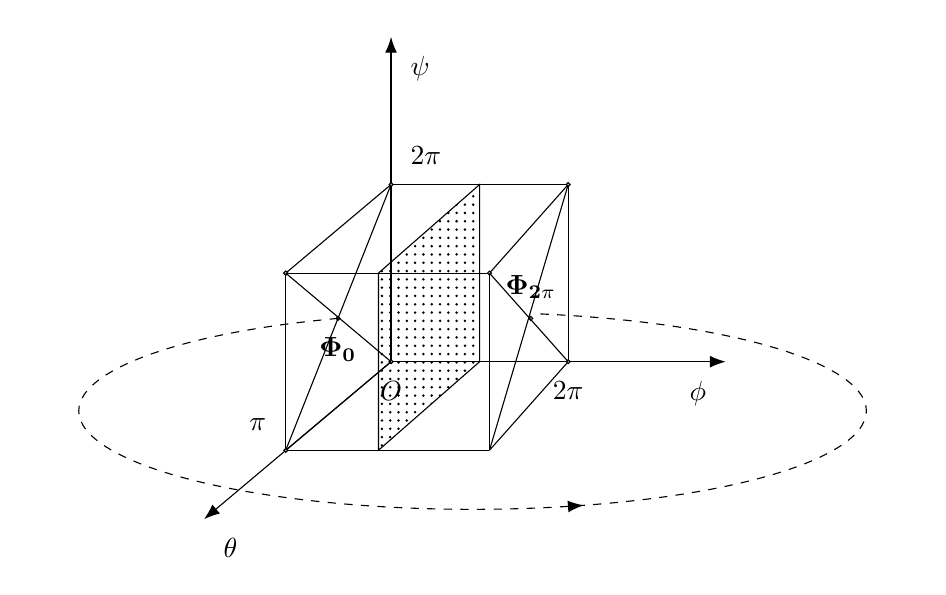
\begin{tikzpicture}[scale=0.25]
\coordinate (O) at (0,0);
\node[label=south :$O$] at (O) {};
\coordinate (X) at (-9.5,-8) {} {};
\coordinate (Y) at (17,0) {} {};
\coordinate (Z) at (0,16.5) {} {};

\coordinate (X0) at (-5.35,-4.5) {} {} ;
\coordinate (Y0) at (9,0) {} ;
\coordinate (Z0) at (0,9) {} {} {} ;
\coordinate (XY) at (5,-4.5) {} {} {} ;
\coordinate (YZ) at (9,9) {} {} ;
\coordinate (XZ) at (-5.35,4.5) {} {};
\coordinate (XYZ) at (5,4.5) {} {} {};


\coordinate (HXY1) at (-0.64,-4.5) {} {} {};
\coordinate (HXY2) at (-0.64,4.5) {} {} {};
\coordinate (HZY1) at (4.5,9) {} {} {};
\coordinate (HZY2) at (4.5,0) {} {} {};


\draw [-{Latex[length=2mm]}] (O) -- (X);
\draw [-{Latex[length=2mm]}] (O) -- (Y);
\draw [-{Latex[length=2mm]}] (O) -- (Z);
\node[label=south east:$\theta$] at (X) {};
\node[label=south west:$\phi$] at (Y) {};
\node[label=south east:$\psi$] at (Z) {};
\node[label=north west:$\pi$] at (X0) {};
\node[label=south :$2\pi$] at (Y0) {};
\node[label=north east:$2\pi$] at (Z0) {};
%\node (Sb) [rectangle, minimum width=3cm, minimum height=1cm,draw=black, pattern color=black, pattern = north east lines]{} ;

\draw [] (X0) -- (XY);
\draw [] (Y0) -- (YZ);
\draw [] (Z0) -- (XZ);
\draw [] (X0) -- (XZ);
\draw [] (Y0) -- (XY);
\draw [] (XY) -- (XYZ);
\draw [] (XZ) -- (XYZ);
\draw [] (YZ) -- (XYZ);
\draw [] (YZ) -- (Z0);
\draw [] (O) -- (Z0);
\draw [] (O) -- (X0);
\draw [] (O) -- (Y0);

\draw[fill=white]  (X0) circle (0.1);
\draw[fill=white]  (Y0) circle (0.1);
\draw[fill=white]  (Z0) circle (0.1);

\draw[fill=white]  (XZ) circle (0.1);
\draw[fill=white]  (YZ) circle (0.1);
\draw[fill=white]  (XZ) circle (0.1);
\draw[fill=white]  (O) circle (0.1);
\draw[fill=white]  (XYZ) circle (0.1);

%\draw[pattern color=black, pattern = dots]  (O) rectangle (YZ) node (v0) {};
%\draw[pattern color=black, pattern = dots]  (X0) rectangle (XYZ) node (v1) {};
\coordinate (plane0) at (7.1,2.2) {};
\coordinate (plane1) at (-2.7,2.2) {};
\draw[fill=white]  (plane1) circle (0.1);
\draw[fill=white]  (plane0) circle (0.1);
%\draw[ decoration={markings, mark=at position 0.75 with {\arrow[scale = 1.]{Latex[length=3mm,reversed]}}},    postaction={decorate}](plane0) .. controls (29.5,-2) and (-28,-4) .. (plane1);
\draw[pattern color=black, pattern = dots]  (HXY1) node (v2) {} -- (HXY2) -- (HZY1) -- (HZY2) -- (HZY2) -- cycle;
\draw  (YZ) edge (XY);
\draw  (XYZ) edge (Y0);
\draw  (XZ) edge (O);
\draw  (Z0) edge (X0);
\node[label=north:$\mathbf{\Phi_{2\pi}}$] at (plane0) {};
\node[label=south:$\mathbf{\Phi_{0}}$] at (plane1) {};
\draw [ dashed,decoration={markings, mark=at position 0.55 with {\arrow[scale = 1.]{Latex[length=2mm]}}},    postaction={decorate}](plane1) arc(-70:261:-20cm and -5cm);
\end{tikzpicture}}
	\
    \subfloat[]{
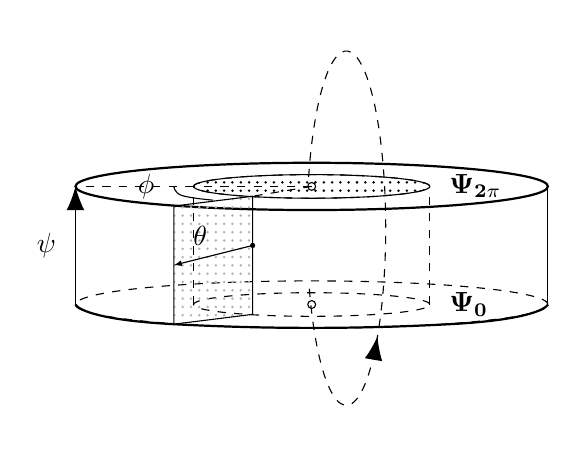
\begin{tikzpicture}[scale=0.5]
\coordinate (O1) at (0,0);
\draw [thick] (O1) ellipse (6 and 0.6);
\coordinate (O2) at (0,-3);
\draw[dashed]  (O2) ellipse (6 and 0.6);
\coordinate (Om) at (0,-1.5);
\coordinate (O1s) at (0,0);
\draw[dashed]  (O1s) ellipse (3 and 0.3);
\coordinate (O2s) at (0,-3);
\draw[dashed]  (O2s) ellipse (3 and 0.3);
\coordinate (Oms) at (0,-1.5);
\draw[pattern color=black, pattern = dots]  (O1) ellipse (3 and 0.3);

%\draw  (O1) ellipse (1 and 0.1);
%\draw[dashed]  (O2) ellipse (1 and 0.1);
\coordinate (Plu) at (-6,0);
\coordinate (Pru) at (6,0);
\coordinate (Pld) at (-6,-3);
\coordinate (Prd) at (6,-3);
\coordinate (Plm) at (-6,-1.5);
\coordinate (Prm) at (6,-1.5);
\coordinate (Plds) at (-3,-3);
\coordinate (Prds) at (3,-3);
\coordinate (Plus) at (-3,0);
\coordinate (Prus) at (3,-0);

\coordinate (Qlu) at (-1,0);
\coordinate (Qru) at (1,0);
\coordinate (Qld) at (-1,-3);
\coordinate (Qrd) at (1,-3);
\draw [-{Latex[length=3mm]}] (Pld) -- (Plu);
\draw [] (Pru) -- (Prd);
\draw [dashed] (Plds) -- (Plus);
\draw [dashed] (Prds) -- (Prus);
%\draw [dashed] (Qlu) -- (Qld);
%\draw [dashed] (Qru) -- (Qrd);
\coordinate (Pu0) at (-1.5,-0.25) {};
\coordinate (Pd0) at (-1.5,-3.25) {};
\coordinate (Pu) at (-3.5,-0.5) {};
\coordinate (Pdl) at (-3.5,-3.5) {} {};
\coordinate (Pdr) at (3.5,-3.5) {} {};
\coordinate (Pmu) at (-3.5,-2) {} {};
\coordinate (Pml) at (-1.5,-1.5) {} {};
\draw[thick]  plot[ smooth,tension=.9] coordinates {(Pld) (Pdl) (Pdr) (Prd)};
\draw [dashed] (Plus) -- (Plu);
\draw[pattern color=gray!60, pattern = dots]  (Pu0) node (v2) {} -- (Pu) -- (Pdl) -- (Pd0) -- (Pu0) -- cycle;
\node[label=west:$\mathbf{\psi}$] at (Plm) {};
\node[label=north east :$\theta$] at (Pmu) {};
\draw  plot[ smooth,tension=.7] coordinates {(-3.5,0) (-3.3,-0.23) (-2.5,-0.35)};
\node[label=west :$\mathbf{\phi}$] at (-3.5,0) {};
\draw [-{Latex[length=1mm]}] (Pml) -- (Pmu);
\draw[fill=white]  (O1) circle (0.1);
\draw[fill=white]  (O2) circle (0.1);
%\draw[ decoration={markings, mark=at position 0.7 with {\arrow[scale = 1.5]{Latex[length=3mm,reversed]}}},    postaction={decorate}](O2) .. controls (3.5,-16.5) and (3.5,11) .. (O1);
\node[label=east:$\mathbf{\Psi_{2\pi}}$] at (Prus) {};
\node[label= east:$\mathbf{\Psi_{0}}$] at (Prds) {};
\draw[fill=black]  (Pml) circle (0.051);
\draw [dashed] (O1) -- (Plus);
\draw [dashed] (O1) -- (Pu0);
\coordinate (Om) at (-0.06,-2.6) {};
\draw [ dashed,decoration={markings, mark=at position 0.32 with {\arrow[scale = 1.]{Latex[length=3mm]}}},    postaction={decorate}](Om) arc (20:345:-1 and -4.5);
\end{tikzpicture}}
    \qquad
    \subfloat[]{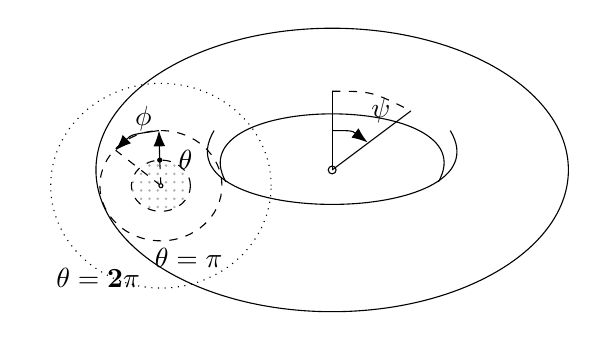
\begin{tikzpicture}[scale=0.5]
\coordinate (O1) at (0,0);
\draw  (O1) ellipse (6 and 3.6);
\coordinate (t1l) at (-3,1.0);
\coordinate (t1r) at (3,1.0);
\coordinate (t1c1) at  (-4.5,-1.5);
\coordinate (t1c2) at (4.5,-1.5);
\draw (t1l) .. controls  (t1c1)  and (t1c2)  .. (t1r);

\coordinate (t2l) at (-2.7,-0.3) {};
\coordinate (t2r) at (2.7,-0.3) {};
\coordinate (t2c1) at (-4,2) {};
\coordinate (t2c2) at (4,2) {};
\draw (t2l) .. controls  (t2c1)  and (t2c2)  .. (t2r);
\draw[fill=white]  (O1) circle (0.1);
\coordinate (a0) at (0,2) {};
\coordinate (a1) at (2,1.5) {} {};
\draw [] (O1) -- (a0);
\draw [] (O1) -- (a1);
\coordinate (ac1) at (1,2) {} {};
\coordinate (ac2) at (1,2) {} {};

\draw [dashed] (a0) .. controls  (ac1)  and (ac2)  .. (a1);
\coordinate (b0) at (0,1.) {};
\coordinate (b1) at (0.9,0.7) {} {};
\coordinate (bc1) at (0.5,1) {} {} {};
\coordinate (bc2) at (0.5,1) {} {} {};
\coordinate (bc3) at (0,0.5) {} {} {} {};
\draw [-{Latex[length=2mm]}]  (b0) .. controls  (bc1)  and (bc2)  .. (b1);
\coordinate (ac3) at (0.5,0.7) {} {} {};
\node[label=north east:$\mathbf{\psi_{}}$] at (ac3) {};
\coordinate (C1) at (-4.35,-.4);
\draw [dashed] (C1) ellipse (1.55 and 1.4);
\draw [dashed,pattern color=gray!60, pattern = dots] (C1) ellipse (0.75 and 0.65);
\draw [dotted] (C1) ellipse (2.8 and 2.6);

\coordinate (C2a) at (-4.38,0.25) {};
\coordinate (C2b) at (-4.4,1) {};
\coordinate (C3b) at (-5.5,0.5) {};
\coordinate (C3a) at (-5,0) {} {};
\draw [dashed] (C1) -- (C2a);
\draw [-{Latex[length=2mm]}] (C2a) -- (C2b);
\draw [dashed] (C1) -- (C3b);
\draw[fill=black]  (C2a) circle (0.051);
%\draw[fill=black]  (C3a) circle (0.051);
\draw[fill=white]  (C1) circle (0.051);
\draw [-{Latex[length=2mm]}] (C2b) .. controls  (-5.1,0.9)  and (-5.1,0.9)  .. (C3b);
\node[label=south east:$\mathbf{\theta}$] at (C2b) {};
\node[label=north east:$\mathbf{\phi}$] at (C3b) {};
\node at (-7,-2.5) {};
\node[label=south east:$\mathbf{\theta = 2\pi}$] at (-7.5,-2) {};
\node at (-3,-1.5) {};
\node[label=south east:$\mathbf{\theta = \pi}$] at (-5,-1.5) {};
\end{tikzpicture}}
\caption{Homeomorphism of the configuration space of a rigid body with fixed point.}
\label{fig:fig_p181}
\end{figure}
Consider figure $5.2 (a)$. We can stretch like an accordion the cuboid along the $\phi$ axis and bent it so that the planes $\phi=0$ and $\phi=2\pi$ join. We get $(b)$,  a torus with square sections. The dimension $\phi$ is dealt with as a point $P\left( \theta, \phi, \psi \right)$ in the configuration space  returns to the same point when varying $\phi$ to $\phi+2k\pi$.\\
We can apply the same procedure of stretching and bending for the $\psi$ dimension so that the planes $\Psi=0$ and $\Psi=2\pi$ join.
We get $(c)$,  a torus-like object.\\
The only dimension left is $\theta$ which our multi-dimensional crippled mind can't find a way to reshape this pseudo-torus so that when varying $\theta$ we can come back to the same point as started.
$$\blacklozenge$$
\newpage
%\setcounter{chapter}{4}
\chapter{Applications to Hydrodynamics, Elasticity, and Electromagnetic radiation}
\pagebreak[4]
\section{p191 - Exercise}
\begin{tcolorbox}
A fluid rotates as a rigid body about the axis of $z_3$ with variable angular velocity $\omega(t)$. Write out explicitly the three Lagrangian equations $\mathbf{6.101}$ and the three Eulerian equations $\mathbf{6.103}$.
\end{tcolorbox}
The motion described reduces to a motion in a $V_2$ plane with $z_3$ a constant for a definite particle.\\\\\\
\textbf{Lagrangian}\\

A particular particle with starting coordinates $\left(z^{(*)}_1,z^{(*)}_2, z^{(*)}_3\right)$ will describe a  circle with radius $\sqrt{z^{(*)2}_1+z^{(*)2}_2}$ in the  plane $V_2$ parallel with the $1,2$ axes.
Taking axis $1$ as reference to determine the instantaneous angle $\theta$ of the vertex $OP$ (origin and particle) we get
\begin{align}
\left\{\begin{array}{l}
z_1 = \sqrt{z^{(*)2}_1+z^{(*)2}_2}\cos\left(\theta(t) + \phi_0\right)\\
z_2 = \sqrt{z^{(*)2}_1+z^{(*)2}_2}\sin\left(\theta(t) + \phi_0\right)\\
z_3 = z^{(*)}_3
\end{array}\right.
\end{align}
with 
\begin{align}
\phi_0 & = \arctan\frac{z^{(*)}_2}{z^{(*)}_1}
\end{align}
Note that $\omega(t)$ is not a constant, so
\begin{align}
\theta(t)&= \int_{0}^{t}\omega(\tau)d\tau
\end{align}
and get 
\begin{align}
\left\{\begin{array}{l}
z_1 = \sqrt{z^{(*)2}_1+z^{(*)2}_2}\cos\left(\int_{0}^{t}\omega(\tau)d\tau + \phi_0\right)\\\\
z_2 = \sqrt{z^{(*)2}_1+z^{(*)2}_2}\sin\left(\int_{0}^{t}\omega(\tau)d\tau + \phi_0\right)\\\\
z_3 = z^{(*)}_3\\\\
\phi_0 = \arctan\frac{z^{(*)}_2}{z^{(*)}_1}
\end{array}\right.
\end{align}
$$\lozenge$$\\
\newpage
\textbf{Eulerian}\\
The equations get simplified and reduce to a motion of a particle on a circle.
\begin{figure}[H]
\centering
\tikzstyle{left-hand-mirror} = [
    draw,
    postaction=decorate, 
    decoration={
        markings,
        mark=between positions 0.015 and 0.98 step 0.1072 with {\draw (0,0)--(60:3pt);}
    }
]   

\begin{tikzpicture}[scale=0.5]
\coordinate (O1) at (0,0);
\draw  (O1) circle (6);
\coordinate (Om) at (0.0,-6) ;
\coordinate  {} {} {};
\coordinate  {} {} {};
\coordinate (NPole) at (0,8.5) {} {};
\coordinate (SPole) at (0,-7.5) {} {};
\draw[-{Latex[length=2mm]}] (SPole) -- (NPole);
\coordinate (P) at (4.2426,4.2426) {} {};
\draw[fill=white]  (P) circle (0.1);
\draw[fill=white]  (O1) circle (0.05);
\draw[dashed] (O1) -- (P);
%\node[label=west:$O$] at (O1) {};
\node[label=east:$P\left(x \text{, } y\right)$] at (P) {};
\coordinate (O2) at (1.5,0) {};
\node[label=north east:$\theta\text{=} \arctan\frac{y}{x}$] at (O2) {};
\draw [dashed, decoration={markings, mark=at position 0.7 with {\arrow[scale = 1.]{Latex[length=2mm]}}},    postaction={decorate}](O2) arc (0:30:2 and 2.0);
\coordinate (F) at (1.5,7) {} {} {};
\draw [-{Latex[length=2mm]}, ] (P) -- (F);
\node[label=east:$\mathbf{\overline{v}}$] at (F) {};
\coordinate (Fp) at (-3,3) {} {} {} {};
\draw [-{Latex[length=2mm]},dashed] (O1) -- (Fp);
\node[label=west:$\mathbf{\overline{v}}$] at (Fp) {};
\tkzMarkRightAngle[size=0.43](F,P,O1);
\tkzMarkRightAngle[size=0.43, ](P,O1,Fp);
\coordinate (x1)at (-7,0) {};
\coordinate (X) at (8.5,0) {} {};
\draw [-{Latex[length=2mm]}] (x1) -- (X);
\node[label=south east:$x$] at (X) {};
\node[label=south east:$y$] at (NPole) {};
\coordinate (xx)at (-3,0) {};
\draw[fill=white]  (xx) circle (0.1);
\coordinate (yy)at (0,3) {};
\draw[fill=white]  (yy) circle (0.1);
\draw [dashed, ] (xx) -- (Fp);
\draw [dashed ] (yy) -- (Fp);
\node[label=south :$-sin\left(\theta\right)$] at (xx) {};
\node[label= east:$cos\left(\theta\right)$] at (yy) {};
\end{tikzpicture}
\caption{Eulerian viewpoint of a spinning fluid}
\label{fig:fig_p191_Exa}
\end{figure}

\begin{align}
\left\{\begin{array}{l}
v_1 = -\sqrt{z^{2}_1+z^{2}_2}\omega(t)\sin\left(\arctan\frac{z^{}_2}{z^{}_1}\right)\\\\
v_2 = \sqrt{z^{2}_1+z^{2}_2}\omega(t)\cos\left(\arctan\frac{z^{}_2}{z^{}_1}\right)\\\\
v_3 = 0
\end{array}\right.
\end{align}
$$\blacklozenge$$
\newpage

\section{p191 - Exercise}
\begin{tcolorbox}
Compute the components of acceleration for the motion described in the preceding exercise.
\end{tcolorbox}
We have
\begin{align}
\left\{\begin{array}{l}
v_1 = -\sqrt{z^{2}_1+z^{2}_2}\omega(t)\sin\left(\arctan\frac{z^{}_2}{z^{}_1}\right)\\\\
v_2 = \sqrt{z^{2}_1+z^{2}_2}\omega(t)\cos\left(\arctan\frac{z^{}_2}{z^{}_1}\right)\\\\
v_3 = 0
\end{array}\right.
\end{align}
and 
\begin{align}
f_r &= \partial_tv_r + v_{r,s}v_s
\end{align}
\begin{align}
&\left\{\begin{array}{l}
\partial_t v_1 = -\sqrt{z^{2}_1+z^{2}_2}\dot{\omega}(t)\sin\left(\arctan\frac{z^{}_2}{z^{}_1}\right)\\\\
\partial_t v_2 = \sqrt{z^{2}_1+z^{2}_2}\dot{\omega}(t)\cos\left(\arctan\frac{z^{}_2}{z^{}_1}\right)\\\\
v_{1,1}= -\omega(t)\left[\frac{z_1}{\sqrt{z^{2}_1+z^{2}_2}}\sin\left(\arctan\frac{z^{}_2}{z^{}_1}\right) -\sqrt{z^{2}_1+z^{2}_2}\cos\left(\arctan\frac{z^{}_2}{z^{}_1}\right)\frac{z_2}{z_1^2}\frac{1}{1+\frac{z_2^2}{z_1^2}}\right]\\\\
v_{1,2}= -\omega(t)\left[\frac{z_2}{\sqrt{z^{2}_1+z^{2}_2}}\sin\left(\arctan\frac{z^{}_2}{z^{}_1}\right) +\sqrt{z^{2}_1+z^{2}_2}\cos\left(\arctan\frac{z^{}_2}{z^{}_1}\right)\frac{1}{z^{}_1}\frac{1}{1+\frac{z_2^2}{z_1^2}}\right]\\\\
v_{2,1}= \omega(t)\left[\frac{z_1}{\sqrt{z^{2}_1+z^{2}_2}}\cos\left(\arctan\frac{z^{}_2}{z^{}_1}\right) +\sqrt{z^{2}_1+z^{2}_2}\sin\left(\arctan\frac{z^{}_2}{z^{}_1}\right)\frac{z_2}{z_1^2}\frac{1}{1+\frac{z_2^2}{z_1^2}}\right]\\\\
v_{2,2}= \omega(t)\left[\frac{z_2}{\sqrt{z^{2}_1+z^{2}_2}}\cos\left(\arctan\frac{z^{}_2}{z^{}_1}\right) -\sqrt{z^{2}_1+z^{2}_2}\sin\left(\arctan\frac{z^{}_2}{z^{}_1}\right)\frac{1}{z^{}_1}\frac{1}{1+\frac{z_2^2}{z_1^2}}\right]\\\\
\end{array}\right.
\end{align}
\begin{align}
&=\left\{\begin{array}{l}
\partial_t v_1 = -\sqrt{z^{2}_1+z^{2}_2}\dot{\omega}(t)\sin\left(\arctan\frac{z^{}_2}{z^{}_1}\right)\\\\
\partial_t v_2 = \sqrt{z^{2}_1+z^{2}_2}\dot{\omega}(t)\cos\left(\arctan\frac{z^{}_2}{z^{}_1}\right)\\\\
v_{1,1}= -\frac{\omega(t)}{\sqrt{z^{2}_1+z^{2}_2}}\left[z_1\sin\left(\arctan\frac{z^{}_2}{z^{}_1}\right) -z_2\cos\left(\arctan\frac{z^{}_2}{z^{}_1}\right)\right]\\\\
v_{1,2}=  -\frac{\omega(t)}{\sqrt{z^{2}_1+z^{2}_2}}\left[z_2\sin\left(\arctan\frac{z^{}_2}{z^{}_1}\right) +z^{}_1\cos\left(\arctan\frac{z^{}_2}{z^{}_1}\right)\right]\\\\
v_{2,1}=  \frac{\omega(t)}{\sqrt{z^{2}_1+z^{2}_2}}\left[z_1\cos\left(\arctan\frac{z^{}_2}{z^{}_1}\right) +z_2\sin\left(\arctan\frac{z^{}_2}{z^{}_1}\right)\right]\\\\
v_{2,2}=  \frac{\omega(t)}{\sqrt{z^{2}_1+z^{2}_2}}\left[z_2\cos\left(\arctan\frac{z^{}_2}{z^{}_1}\right) -z^{}_1\sin\left(\arctan\frac{z^{}_2}{z^{}_1}\right)\right]\\\\
\end{array}\right.
\end{align}
and get
\begin{align}
v_{1,s}v_s &= \left\{\begin{array}{l}
-\sqrt{z^{2}_1+z^{2}_2}\omega(t)\sin\left(\arctan\frac{z^{}_2}{z^{}_1}\right)\frac{\omega(t)}{\sqrt{z^{2}_1+z^{2}_2}}\left[z_1\sin\left(\arctan\frac{z^{}_2}{z^{}_1}\right) -z_2\cos\left(\arctan\frac{z^{}_2}{z^{}_1}\right)\right]\\\\
-\sqrt{z^{2}_1+z^{2}_2}\omega(t)\cos\left(\arctan\frac{z^{}_2}{z^{}_1}\right)\frac{\omega(t)}{\sqrt{z^{2}_1+z^{2}_2}}\left[z_2\sin\left(\arctan\frac{z^{}_2}{z^{}_1}\right) +z^{}_1\cos\left(\arctan\frac{z^{}_2}{z^{}_1}\right)\right]
\end{array}\right.\\
&=-z_1\omega^2(t)
\end{align}
\begin{align}
v_{2,s}v_s &= \left\{\begin{array}{l}
\sqrt{z^{2}_1+z^{2}_2}\omega(t)\sin\left(\arctan\frac{z^{}_2}{z^{}_1}\right)\frac{\omega(t)}{\sqrt{z^{2}_1+z^{2}_2}}\left[z_1\cos\left(\arctan\frac{z^{}_2}{z^{}_1}\right) +z_2\sin\left(\arctan\frac{z^{}_2}{z^{}_1}\right)\right]\\\\
+\sqrt{z^{2}_1+z^{2}_2}\omega(t)\cos\left(\arctan\frac{z^{}_2}{z^{}_1}\right)\frac{\omega(t)}{\sqrt{z^{2}_1+z^{2}_2}}\left[z_2\cos\left(\arctan\frac{z^{}_2}{z^{}_1}\right) -z^{}_1\sin\left(\arctan\frac{z^{}_2}{z^{}_1}\right)\right]\\\\
\end{array}\right.\\
&= z_2\omega^2(t)
\end{align}
giving with the second derivative term
\begin{align}
&=\left\{\begin{array}{l}
f_1 = -\dot{\omega}(t)\sqrt{z^{2}_1+z^{2}_2}\sin\left(\arctan\frac{z^{}_2}{z^{}_1}\right)-z_1\omega^2(t)\\\\\\
f_2 = \dot{\omega}(t)\sqrt{z^{2}_1+z^{2}_2}\cos\left(\arctan\frac{z^{}_2}{z^{}_1}\right)+z_2\omega^2(t)\\\\
f_3=0
\end{array}\right.
\end{align}
$$\blacklozenge$$
\newpage


\section{p193 - Exercise}
\begin{tcolorbox}
Verify that the operator $\frac{\partial}{\partial t}$ does not alter tensor character.
\end{tcolorbox}
Be $X^r$ and $Y^r$, two tensors so that $I=X_rY^r$ is an invariant. Obviously, $\frac{\partial I}{\partial t}$ will also be invariant and 
\begin{align}
\frac{\partial I}{\partial t}= \frac{\partial X_r}{\partial t}Y^r+X_r\frac{\partial Y^r}{\partial t}
\end{align}
Meaning that the right side is a sum of two invariants, from which we conclude (see page 20, $\mathbf{1.607}$) that $\frac{\partial X_r}{\partial t}$ and $\frac{\partial Y^r}{\partial t}$ are tensors.
$$\blacklozenge$$
\newpage

\section{p193 - Clarification to 6.112}
\begin{tcolorbox}
$$\mathbf{6.112.}\spatie \int Fn_rdS = \int F_{,r}dV$$
\end{tcolorbox}
Green's theorem is generally presented in the form
$$\int\overline{F}.\overline{n}dS = \int \overline{\nabla}. \overline{F}dV$$or
$$\int F_rn_rdS = \int F_{r,r}dV$$
We can define $$\overline{F} = F\overline{1}_r$$
 $\overline{F}.\overline{n}$  will then become $Fn_r$ while $\overline{\nabla}. \overline{F}$ will become $\partial_r F$, giving the expression $\mathbf{6.112.}$.
 $$\blacklozenge$$
\newpage



\section{p196 - Exercise}
\begin{tcolorbox}
Write out $\mathbf{6.126}$ and $\mathbf{6.127b}$ explicitly for spherical polar coordinates.
\end{tcolorbox}
For spherical polar coordinates we have 
\begin{align}
(v^r) = \left(\begin{matrix}\dot{r}\\r\dot{\theta}\\r\sin\theta\dot{\phi} \end{matrix}\right)
\end{align}
and (see $\mathbf{2.546}$ page 58):
\begin{align}
v^r_{|r} &= \frac{1}{r^2}\partial_r\left(r^2v^1\right)+\frac{1}{\sin\theta}\partial_{\theta}\left(\sin\theta v^2\right)+\partial_{\phi} v^3\\
&=  \frac{1}{r^2}\left(2rv^1+r^2\partial_rv^1\right)+\frac{1}{\sin\theta}\left(v^2\cos\theta + \sin\theta\partial_{\theta}v^2\right)\\
&= \frac{2}{r}\dot{r}+r\dot{\theta}\cot \theta 
\end{align}
and 
\begin{align}
&\partial_t \rho+ \left(\rho v^r\right)_{|r} =0\\
\Leftrightarrow\spatie &\partial_t\rho+ \rho_{|r}v^r+\rho v^r_{|r} =0\\
\Leftrightarrow\spatie &\dv{\rho}{t}+\rho \left(\frac{2}{r}\dot{r}+r\dot{\theta}\cot \theta \right) =0
\end{align}
 $$\blacklozenge$$
\newpage


\section{p198 - Exercise}
\begin{tcolorbox}
If $\epsilon^{rmn}$ is defined in precisely the same way as $\epsilon_{rmn}$, prove that $$ \epsilon^{'uvw}= J\epsilon^{rmn}\frac{\partial x^{'u}}{\partial x^r}\frac{\partial x^{'v}}{\partial x^m}\frac{\partial x^{'w}}{\partial x^n}$$
\end{tcolorbox}
We follow the pretty same line of reasoning as for $\epsilon_{rst}$. Going from $x^{'r}$ to $x^{s}$ we have (expanding the determinant of the inverse Jacobian along the rows instead of the columns):
\begin{align}
J^{-1}=\left|\frac{\partial x^{'p}}{\partial x^{q}}\right|&= \epsilon^{rmn}\frac{\partial x^{'1}}{\partial x^r}\frac{\partial x^{'2}}{\partial x^m}\frac{\partial x^{'3}}{\partial x^n}\\
\times \epsilon^{uvw}\spatie J^{-1}\epsilon^{uvw}&= \epsilon^{rmn}\frac{\partial x^{'u}}{\partial x^r}\frac{\partial x^{'v}}{\partial x^m}\frac{\partial x^{'w}}{\partial x^n}\\
\times J\spatie\epsilon^{uvw}&= J\epsilon^{rmn}\frac{\partial x^{'u}}{\partial x^r}\frac{\partial x^{'v}}{\partial x^m}\frac{\partial x^{'w}}{\partial x^n}\\ 
\end{align}
 $$\blacklozenge$$
\newpage



\section{p198 - Exercise}
\begin{tcolorbox}
Prove that  $\frac{\epsilon^{rmn}}{\sqrt{a}}$ is an (absolute) contravariant tensor of the third order.
\end{tcolorbox}
\begin{align} 
\sqrt{a^{'}} &= J\sqrt{a}\\
\epsilon^{'uvw}&= J\epsilon^{rmn}\frac{\partial x^{'u}}{\partial x^r}\frac{\partial x^{'v}}{\partial x^m}\frac{\partial x^{'w}}{\partial x^n}\\
\text{(1)  in (2)} \spatie \epsilon^{'uvw}&= \frac{\sqrt{a^{'}}}{\sqrt{a^{}}}\epsilon^{rmn}\frac{\partial x^{'u}}{\partial x^r}\frac{\partial x^{'v}}{\partial x^m}\frac{\partial x^{'w}}{\partial x^n}\\
\Rightarrow \spatie \frac{\epsilon^{'uvw}}{\sqrt{a^{'}}}&= \frac{\epsilon^{rmn}}{\sqrt{a}}\frac{\partial x^{'u}}{\partial x^r}\frac{\partial x^{'v}}{\partial x^m}\frac{\partial x^{'w}}{\partial x^n}
\end{align}
which is the required transformation rule for a "normal" (absolute) tensor.
 $$\blacklozenge$$
\newpage


\section{p199 - Clarification to pressure invariance to direction of the surface element.}
\begin{tcolorbox}
Pressure is independent of the direction
\end{tcolorbox}
\begin{figure}[H]%
    \centering
    \subfloat[]{\tdplotsetmaincoords{80}{160}
\begin{tikzpicture}[tdplot_main_coords, >=Latex]
\tikzmath{\aax=3.84;\bby=6;\ccz=4;\a = (\bby+\bby)/4;\d=-8.5;\e=4;};
\aax, \bby,\ccz;
\coordinate (O) at (0,0,0);
\coordinate (A) at (0,0,\ccz);
\coordinate (B) at (0,\bby,0);
\coordinate (C) at (\aax,0,0);
\coordinate (x) at (1.5*\aax,0,0);
\coordinate (y) at (0,1.5*\bby,0);
\coordinate (z) at (0,0,1.5*\ccz);

\coordinate (xy) at (\aax/3,\bby/3,0);
\draw [fill=white] (xy) circle (2pt) node[above right] (n1) {$$};
\coordinate (xz) at (\aax/3,0,\ccz/3);
\draw [fill=white] (xz) circle (2pt) node[above right] (n1) {$$};
\coordinate (yz) at (0,\bby/3,\ccz/3);
\draw [fill=white] (yz) circle (2pt) node[above right] (n1) {$$};
\coordinate (xyz) at (\aax/3,\bby/3,\ccz/3);
\draw [fill=gray] (xyz) circle (2pt) node[above right] (n1) {$$};

\coordinate (nxy) at (\aax/3,\bby/3,-2);
\coordinate (nxyO) at (\aax/3,\bby/3,-0.2);
\draw[dashed, thick](xy)--(nxyO);
\draw[-Latex,very thick](nxyO)--(nxy);
\coordinate (nxz) at (\aax/3,-5,\ccz/3);
\coordinate (nxzO) at (\aax/3,-2.5,\ccz/3);
\draw[dashed,very thick](xz)--(nxzO);
\draw[-Latex,very thick](nxzO)--(nxz);
\coordinate (nyz) at (-2,\bby/3,\ccz/3);
\coordinate (nyzO) at (-0.5,\bby/3,\ccz/3);
\draw[dashed,very thick](yz)--(nyzO);
\draw[-Latex,very thick](nyzO)--(nyz);

\coordinate (nxyz) at (3*\aax/3,3*\bby/3,3*\ccz/3);
\draw[-Latex, very thick](xyz)--(nxyz);
\node[anchor = south east] at (nxy){$dS_z$};
\node[anchor = south east] at (nxz){$dS_y$};
\node[anchor = south east] at (nyz){$dS_x$};
\node[anchor = south east] at (nxyz){$dS_t$};

\coordinate (yzp) at (3*\aax/3,\bby/3,\ccz/3);
\draw[-Latex,](xyz)--(yzp);
\node[anchor = south east] at (yzp){$$};

\coordinate (xyp) at (\aax/3,\bby/3,3.1*\ccz/3);
\draw[-Latex,](xyz)--(xyp);
\node[anchor = south east] at (xyp){$$};

\coordinate (xzp) at (\aax/3,3*\bby/3,\ccz/3);
\draw[-Latex, ](xyz)--(xzp);
\node[anchor = north west] at (xzp){$$};

\coordinate (pz) at (\aax/3,\bby/3,3.1*\ccz/3);
\draw[ dashed](nxyz)--(pz);
\draw [fill=white] (pz) circle (1pt)node[above left] (pz) {$\gamma_z$};

\coordinate (pxy) at (3.*\aax/3,3*\bby/3,\ccz/3);
\draw[ dashed](nxyz)--(pxy);
\draw[ dashed](xyz)--(pxy);
\draw [fill=white] (pxy) circle (1pt) {};

\coordinate (px) at (3*\aax/3,\bby/3,\ccz/3);
\draw[ dashed](pxy)--(px);
\draw [fill=white] (px) circle (1pt) node[above left] (px) {$\gamma_x$};
\coordinate (py) at (\aax/3,3*\bby/3,\ccz/3);
\draw[ dashed](pxy)--(py);
\draw [fill=white] (py) circle (1pt)node[above right] (py) {$\gamma_y$};


\draw[-Latex](O)--(x);
\node[anchor = south east] at (x){x};
\draw[-Latex](O)--(y);
\node[anchor = south east] at (y){y};
\draw[-Latex](O)--(z);
\node[anchor = south east] at (z){z};

\draw[very thick,](A)--(B)--(C)--cycle;

\draw[dashed, very thick](O)--(B);
\draw[dashed, very thick](O)--(C);
\draw[dashed,very thick](O)--(A);

\node[anchor = south west] at (A){A};
\node[anchor = north east] at (O){o};
\node[anchor = north east] at (C){C};
\node[anchor = south west ] at (B){B};

\end{tikzpicture}    }
    \quad
        \subfloat[]{\tdplotsetmaincoords{80}{160}
\begin{tikzpicture}[scale = 0.8,tdplot_main_coords, >=Latex]
\tikzmath{\aax=3.84;\bby=6;\ccz=4;\a = (\bby+\bby)/4;\d=-8.5;\e=4;};
\aax, \bby,\ccz;
\coordinate (O) at (0,0,0);
\coordinate (A) at (0,0,\ccz);
\coordinate (B) at (0,\bby,0);
\coordinate (C) at (\aax,0,0);
\coordinate (x) at (1.5*\aax,0,0);
\coordinate (y) at (0,1.5*\bby,0);
\coordinate (z) at (0,0,1.5*\ccz);

\coordinate (xyz) at (\aax/3,\bby/3,\ccz/3);
\draw [fill=gray] (xyz) circle (2pt) node[above right] (n1) {$$};


\coordinate (nxyz) at (3*\aax/3,3*\bby/3,3*\ccz/3);
\draw[-Latex, very thick](xyz)--(nxyz);
\node[anchor = south east] at (nxyz){$dS_t$};

\coordinate (yzp) at (3*\aax/3,\bby/3,\ccz/3);
\draw[-Latex,](xyz)--(yzp);
\node[anchor = south east] at (yzp){$$};

\coordinate (xyp) at (\aax/3,\bby/3,3.1*\ccz/3);
\draw[-Latex,](xyz)--(xyp);
\node[anchor = south east] at (xyp){$$};

\coordinate (xzp) at (\aax/3,3*\bby/3,\ccz/3);
\draw[-Latex, ](xyz)--(xzp);
\node[anchor = north west] at (xzp){$$};
\node[anchor = north east] at (xyz){$q_{t}$};

\coordinate (pz) at (\aax/3,\bby/3,3.1*\ccz/3);

\draw [fill=white] (pz) circle (1pt)node[above left] (pz) {$\gamma_z$};

\coordinate (pxy) at (3.*\aax/3,3*\bby/3,\ccz/3);


\coordinate (px) at (3*\aax/3,\bby/3,\ccz/3);

\draw [fill=white] (px) circle (1pt) node[above left] (px) {$\gamma_x$};
\coordinate (py) at (\aax/3,3*\bby/3,\ccz/3);

\draw [fill=white] (py) circle (1pt)node[above right] (py) {$\gamma_y$};


\draw[-Latex](O)--(x);
\node[anchor = south east] at (x){x};
\draw[-Latex](O)--(y);
\node[anchor = south east] at (y){y};
\draw[-Latex](O)--(z);
\node[anchor = south east] at (z){z};

\draw[,](A)--(B)--(C)--cycle;
\draw[](A)--(O)--(C)--cycle;
\draw[](A)--(O)--(B)--cycle;
\draw[](O)--(B)--(C)--cycle;

\node[anchor = south west] at (A){A};
\node[anchor = south west] at (O){o};
\node[anchor = north east] at (C){C};
\node[anchor = south west ] at (B){B};
%\draw[-Latex, ultra thick](xyz)--(A);
\coordinate (Ht) at (\aax/2,\bby/2,0);
\draw[dashed,ultra thick](A)--(Ht);
\draw [fill=white] (Ht) circle (1pt)node[below left] (Ht) {$h$};
\draw[dashed,ultra thick](O)--(Ht);

\end{tikzpicture}    }
    \quad
        \subfloat[]{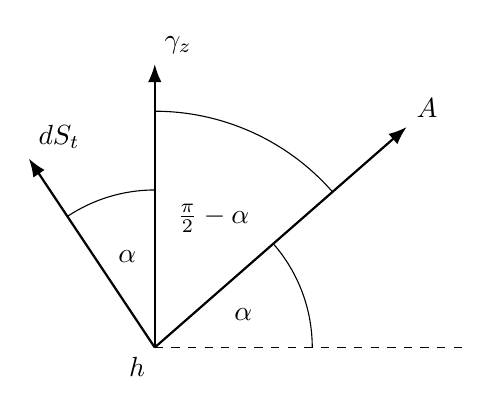
\begin{tikzpicture}[scale = 0.8]
\coordinate (O) at (0,0);
\node[anchor = north east ] at (O){$h$};
\coordinate (ds) at (-2,3);
\draw[-Latex,thick] (O)--(ds);
\node[anchor = south west ] at (ds){$dS_t$};
\coordinate (A) at (4,3.5) {};
\draw[-Latex,thick] (O)--(A);
\node[anchor = south west ] at (A){$A$};
\coordinate (gamma) at (0,4.5) {};
\draw[-Latex,thick] (O)--(gamma);
\node[anchor = south west ] at (gamma){$\gamma_z$};
 \draw pic[draw,,angle radius=3cm,"$\frac{\pi}{2}-\alpha$"] {angle=A--O--gamma};
  \draw pic[draw,,angle radius=2cm,"$\alpha$"] {angle=gamma--O--ds};
  \coordinate (P) at (5,0);
  \draw[dashed] (O)--(P);
  \draw pic[draw,,angle radius=2cm,"$\alpha$"] {angle=P--O--A};
\end{tikzpicture}
}
    \quad
\caption{Pressure on a trirectangular tetrahedron}
\label{fig:fig_p199}
\end{figure}
To see that the pressure is independent of the direction of the surface element on which we measure it, let's consider a trirectangular tetrahedron $OABC$ as  depicted in figure $5.2(a)$. Let's define $P_x,P_y,P_z, P_t$ the pressure measured on the $4$ surfaces with normal vectors $dS_x,dS_y,dS_z,dS_t$. Let's neglect second order terms due to acceleration and external forces. For the forces along axis $z$ (the same reasoning is valid for the two others) we will have $P_zdS_z= P_tdS_t\gamma_z$ where $\gamma_z$ is the cosine of the angle formed by  normal on $dS_t$ and the z-axis.\\
Let's investigate the relationship between $dS_t$ and $dS_x,dS_y,dS_z$.\\
 Be $hA$ the line element lying in the plane $ABC$ (see figure $5.2(b)$) and $hO$ the line element lying in the plane $OBC$. As the area of a triangle $=\half\times base \times perpendicular \ height$ we get $dS_z = \half |hO||BC|$. But $|hO|= |hA|\cos\alpha$  (see figure $5.2(c)$) and so $dS_z = \half |BC||hA|\cos\alpha = dS_t\gamma_z$
 and get 
\begin{align}
&P_zdS_z= P_tdS_t\gamma_z\\ 
\Rightarrow \spatie & P_z dS_t\gamma_z= P_tdS_t\gamma_z\\ 
\Rightarrow \spatie & P_z = P_t
\end{align}

 $$\blacklozenge$$
\newpage
\section{p201 - Exercise}
\begin{tcolorbox}
Write down the contravariant form of $\mathbf{6.147}$
$$\mathbf{6.147} \spatie \partial_t v_r + v_s v_{r|s} = X_r - \rho^{-1} p_{,r}$$
\end{tcolorbox}
\begin{align}
\mathbf{6.147} \spatie \partial_t v_r + v_s v_{r|s} &= X_r - \rho^{-1} p_{,r}\\
\times a^{mr}\spatie \partial_t a^{mr} v_r + v_s a^{mr}v_{r|s} &= a^{mr}X_r - \rho^{-1} a^{mr}p_{,r}
\end{align}
By $\mathbf{2.527}$ page 53 we  have $a^{rs}_{|t}=0$ and thus 
\begin{align}
v^{r}_{|s}= \left(a^{mr}v_{r}\right)_{|s} &= \left(a^{mr}\right)_{|n}v_{r}+a^{mr}v_{r|s}= a^{mr}v_{r|s} \\
(2) \Rightarrow \spatie \partial_t  v^m + v_s v^{m}_{|s} &= X^m - \rho^{-1} a^{mr}p_{,r}\\
(2) \Rightarrow \spatie \partial_t  v^m + v_s v^{m}_{|s} &= X^m - \rho^{-1} p^{'}_{,r}
\end{align}
Note that $p_{,r}$ in $(1)$ and $(5)$ are not the same vector function as $p_{,r}$ can be written as $\overline{\nabla}p$ which is coordinate system  dependent.
 $$\blacklozenge$$
\newpage

\section{p202 - Exercise}
\begin{tcolorbox}
Verify by means of  $\mathbf{3.204}$ that $\mathbf{6.157}$ and $\mathbf{6.156}$  are the same equation.
\end{tcolorbox}
\begin{align}
\left\{\begin{array}{lll}
\mathbf{3.204}&\spatie&\Gamma^{n}_{rn} = \half\partial_r\log a = \partial_r\log \sqrt{a}\\
\mathbf{6.157}&\spatie&\left(\sqrt{a}a^{mn}\phi_{,m}\right)_{,n}=0\\
\mathbf{6.156}&\spatie&a^{mn}\phi_{|mn}=0
\end{array}\right.
\end{align}
Considering also
\begin{align}
\left\{\begin{array}{l}
a^{mn}_{|k}=0\\
T^m_{|n}= \partial_n T_m+\Gamma^{m}_{kn}T_k
\end{array}\right.
\end{align}
So $\mathbf{6.156}$ can written as
\begin{align}
& a^{mn}\phi_{|mn}=0\\
\Leftrightarrow\spatie & \left(a^{mn}\phi_{|m}\right)_{|n}=0\\
T^n = a^{mn}\phi_{|m}\spatie\Rightarrow\spatie &\partial_n T^n+\Gamma^{n}_{kn}T^k=0\\
\Rightarrow\spatie &\partial_n \left(a^{mn}\phi_{|m}\right)+\Gamma^{n}_{kn}a^{pk}\phi_{|p}=0\\
\Leftrightarrow\spatie &\partial_n \left(a^{mn}\right) \phi_{,m}+a^{mn}\phi_{,mn}+\Gamma^{n}_{kn}a^{pk}\phi_{,p}=0\\
\text{(2)}\quad \Rightarrow\spatie &\partial_n \left(a^{mn}\right) \phi_{,m}+a^{mn}\phi_{,mn}+\partial_k\log \sqrt{a}a^{pk}\phi_{,p}=0\\
\Leftrightarrow\spatie &\left(a^{mn}_{,n}\right) \phi_{,m}+a^{mn}\phi_{,mn}+\frac{1}{\sqrt{a}}\left(\sqrt{a}a^{pk}\right)_{,k}\phi_{,p}=0\\
\Leftrightarrow\spatie &\sqrt{a} \phi_{,m}\left(a^{mn}\right)_{,n}+\sqrt{a}a^{mn}\phi_{,mn}+a^{mn}\phi_{,m}\left(\sqrt{a}\right)_{,n}=0\\
\Leftrightarrow\spatie &\left(\sqrt{a}a^{mn}\phi_{,m}\right)_{,n}=0
\end{align}
 $$\blacklozenge$$
\newpage


\section{p205 - Exercise}
\begin{tcolorbox}
Show that a small strain is a rigid body displacement if, and only if, $e_{rs}=0$. In the case of finite strain, deduce form $\mathbf{6.206}$ the conditions which must be satisfied by the partial derivatives of the displacement in order that it may b a rigid body displacement.
\end{tcolorbox}
\textbf{Suppose we deal with  a rigid body.} Then the position of two particles of the rigid body are given by

\begin{align}
\left\{\begin{array}{l}
p_r=z_r+u_r(z)\\
p^{'}_r=z^{'}_r+u_r(z^{'})\\
\end{array}\right.
\end{align}
and
\begin{align}
\left\{\begin{array}{l}
L_0= z_r-z^{'}_r \\
L_1 = z^{'}_r+u_r(z^{'})-z_r-u_r(z)  
\end{array}\right.
\end{align}
A rigid body means $L_1=L_0$, giving $u_r(z^{'})=u_r(z^{})$ i.e $u_r(z^{})$ is a constant and thus $u_{r,s}(z^{})=0$.\\
As $e_{rs}=\half\left(u_{r,s}(z^{})+u_{s,r}(z^{})\right)$ we get $e_{rs}=0$\\\\
\textbf{Suppose now that $e_{rs}=0$}\\
We have $e= e_{rs}\lambda_r\lambda_s = 0$ and $e= u_{r,s}(z^{})\lambda_r\lambda_s $
As the $\lambda_r$ are arbitrary, in the sense that we are free to choose whatever curve to approach the initial point, we conclude that $u_{r,s}(z^{})=0$ . So$u_{r}(z^{})$ is a constant, meaning that the mutual distance between two arbitrary points, do not change. The body is a rigid body.
 $$\lozenge$$
 For a finite strain we have $\mathbf{6.206}$:
 \begin{align}
 \lim \frac{L_1^2-L_0^2}{L_0^2}=2 u_{r,s}(z^{})\lambda_r\lambda_s + u_{m,r}(z^{})u_{m,s}(z^{})\lambda_r\lambda_s
 \end{align}
 This limit is $0$ and so we get as condition
  \begin{align}
 \left(2 u_{r,s}(z^{}) + u_{m,r}(z^{})u_{m,s}(z^{})\right)\lambda_r\lambda_s=0
 \end{align}
 As the $\lambda_r$ are arbitrary, in the sense that we are free to choose whatever curve to approach the initial point, we conclude that $2 u_{r,s}(z^{}) + u_{m,r}(z^{})u_{m,s}(z^{})$ must be zero.
 $$2 u_{r,s}(z^{}) + u_{m,r}(z^{})u_{m,s}(z^{})=0$$
 $$\blacklozenge$$
\newpage

\section{p207 - Clarification}
\begin{tcolorbox}
Then, clearly, since the the volume of the tetrahedron is less than $a^3$,\\\\
$\mathbf{6.217}\spatie \displaystyle \lim_{a \to 0} \frac{1}{a^2} \dv{M_r}{t}=0,\quad \displaystyle \lim_{a \to 0} \frac{1}{a^2} \int X_rdV=0$
$$\vdots$$
But  $\displaystyle \lim_{a \to 0} \frac{S}{a^2}$ is not zero,...
\end{tcolorbox}
First, note that the volume of  a trirectangular tetrahedron is $V=\frac{1}{6}abc$ with $a,b,c$ the bases of the 3 rectangular triangles (see clarification for page 199), so if $a\ge b,c$ we have  $V< a^3$.\\
There is no assurance that $\displaystyle \lim_{a \to 0} \frac{1}{a^3} \dv{M_r}{t}=0$. Indeed, consider $\mathbf{5.334}$. For a continuous medium, this equation can be written as
\begin{align}
I_{st} &= \int_{V}\rho\epsilon_{ptq}\epsilon_{psn}z_sz_tdV
\end{align} 
If $V$ goes to zero, the quantities under the integral can be approximated by constant values and hence, the dynamics of the tetrahedron are govern by
\begin{align}
&\displaystyle \lim_{V \to 0}I_{st} = \rho\epsilon_{ptq}\epsilon_{psn}z_sz_t V\\
\mathbf{5.332}\text{:}\spatie &\dv{I_{st}\omega_t}{t}= M_s\\
\Rightarrow\spatie &\lim_{V \to 0} \dv{M_s}{t} = \lim_{V \to 0}V\dv{\left(\rho\epsilon_{ptq}\epsilon_{psn}z_sz_t\omega_t\right)}{t} \\
\Rightarrow\spatie &\lim_{a \to 0} \frac{1}{a^3}\dv{M_s}{t} = \lim_{a \to 0}\frac{1}{a^3}V\dv{\left(\rho\epsilon_{ptq}\epsilon_{psn}z_sz_t\omega_t\right)}{t} \\
\Rightarrow\spatie &\lim_{a \to 0} \frac{1}{a^3}\dv{M_s}{t} < \lim_{a \to 0}\frac{1}{a^3}a^3\dv{\left(\rho\epsilon_{ptq}\epsilon_{psn}z_sz_t\omega_t\right)}{t} \\
\Rightarrow\spatie &\lim_{a \to 0} \frac{1}{a^3}\dv{M_s}{t} < \lim_{a \to 0}\dv{\left(\rho\epsilon_{ptq}\epsilon_{psn}z_sz_t\omega_t\right)}{t}
\end{align}
but there is no reason to admit that $\displaystyle \lim_{V \to 0}\dv{\left(\rho\epsilon_{ptq}\epsilon_{psn}z_sz_t\omega_t\right)}{t}=0$. \\
On the other hand, replacing $a_3$ with $a^2$ in $(5)$ gives 
\begin{align}
&\lim_{a \to 0} \frac{1}{a^2}\dv{M_s}{t} = \lim_{a \to 0}\frac{1}{a^2}V\dv{\left(\rho\epsilon_{ptq}\epsilon_{psn}z_sz_t\omega_t\right)}{t} \\
\Rightarrow\spatie &\lim_{a \to 0} \frac{1}{a^2}\dv{M_s}{t} < \lim_{a \to 0}\frac{1}{a^2}a^3\dv{\left(\rho\epsilon_{ptq}\epsilon_{psn}z_sz_t\omega_t\right)}{t} \\
\Rightarrow\spatie &\lim_{a \to 0} \frac{1}{a^2}\dv{M_s}{t} < \lim_{a \to 0}a\dv{\left(\rho\epsilon_{ptq}\epsilon_{psn}z_sz_t\omega_t\right)}{t}\\
\Rightarrow\spatie &\lim_{a \to 0} \frac{1}{a^2}\dv{M_s}{t} =0
\end{align}
For $ \displaystyle \lim_{a \to 0} \frac{1}{a^2} \int X_rdV=0$ the reasoning is even simpler as for a volume going to zero , we can consider $X_r$ as constant and thus 
\begin{align}
 \displaystyle \lim_{a \to 0} \frac{1}{a^2} \int X_rdV=\displaystyle \lim_{a \to 0} \frac{1}{a^2}  X_r \int dV < \displaystyle \lim_{a \to 0} \frac{1}{a^2}  X_r a^3 = 0
\end{align}
$$\lozenge$$
\textbf{But  $\displaystyle \lim_{a \to 0} \frac{S}{a^2}$ is not zero,...}\\\\
Be $S_t$ the area of the "sloped" triangle in the tetrahedron. Then, the total area of the tetrahedron is:
\begin{align}
&S= \half\left(ab + bc + ac \right) + S_t\\
&S_t > \half ab\text{,   }S_t > \half bc\text{,   }S_t > \half ac\\
\Rightarrow \spatie & S>  \half\left(ab + bc + ac \right) + \half ab\\
\Rightarrow \spatie & \frac{S}{a^2}>  \half\left( \frac{bc}{a^2} + \frac{c}{a} \right) + b
\end{align}
If we shrink the tetrahedron uniformly and put $a=\epsilon a_0, b=\epsilon b_0, c=\epsilon c_0$ then $(16)$ can be written as 
\begin{align}
\lim_{\epsilon \to 0}\frac{S}{a^2}>   \half\left( \frac{b_0c_0}{a_0^2} + \frac{c_0}{a_0} \right) + b_0\lim_{\epsilon \to 0}\epsilon 
\end{align}
which is indeed not zero.
 $$\blacklozenge$$
\newpage

\section{p208 - Exercise}
\begin{tcolorbox}
Show that the stress across a plane $z_1 = \text{const.}$ has the components $E_{11}, \ E_{21}, \ E_{31}$. What are the components across planes $z_2 = \text{const.}$ and $z_3 = \text{const.}$?
\end{tcolorbox}
\begin{align}
\mathbf{6.223} \spatie T_r = E_{rs}n_s
\end{align}
So for the the stress across a plane $z_1 = \text{const.}$, we have $n_1=1, \ n_2=0, \ n_3 = 0$ and so 
\begin{align}
T_r\left(z_1 = \text{const.}\right) = \left(\begin{matrix}E_{11}\\E_{21}\\E_{31}\end{matrix}\right)
\end{align}
For the the stress across a plane $z_2 = \text{const.}$, we have $n_1=0, \ n_2=1, \ n_3 = 0$ and for the the stress across a plane $z_3 = \text{const.}$, we have $n_1=0, \ n_2=0, \ n_3 = 1$ and so
\begin{align}
&T_r\left(z_2 = \text{const.}\right) = \left(\begin{matrix}E_{12}\\E_{22}\\E_{32}\end{matrix}\right)\\
&T_r\left(z_3 = \text{const.}\right) = \left(\begin{matrix}E_{13}\\E_{23}\\E_{33}\end{matrix}\right)\
\end{align}
 $$\blacklozenge$$
\newpage
%\setcounter{chapter}{6}
\chapter{Relative tensors, ideas of volume, Green-Stokes theorems.}
\pagebreak[4]

\section{p241 - Exercise}
\begin{tcolorbox}
If $b_{rs}$ is an absolute tensor, show that the determinant $\left|b_{rs}\right|$ is a relative invariant of weight $2$. What are the tensor characters of $\left|c^{rs}\right|$ and $\left|f^r_{s}\right|$?
\end{tcolorbox}
As $b_{rs}$ is an absolute tensor, we have 
\begin{align}
b^{'}_{uv}&= b_{rs}\pdv{x^r}{x^{'u}}\pdv{x^s}{x^{'v}}
\end{align}
Hence,
\begin{align}
\left|b^{'}_{uv}\right|&= \left|b_{rs}\right|\left|\pdv{x^r}{x^{'u}}\right|\left|\pdv{x^s}{x^{'v}}\right|
\end{align}
and as $J= \left|\pdv{x^k}{x^{'s}}\right|$ we get 
\begin{align}
\left|b^{'}_{uv}\right|&= J^2\left|b_{rs}\right|
\end{align}
Conclusion, $\left|b_{rs}\right|$ is a relative invariant of weight $ 2$.
$$\lozenge$$
As $c^{rs}$ is an absolute tensor, we have 
\begin{align}
c^{'uv}&= c^{rs}\pdv{x^{'u}}{x^r}\pdv{x^{'v}}{x^s}
\end{align}
Hence,
\begin{align}
\left|c^{'uv}\right|&= \left|c^{rs}\right|\left|\pdv{x^{'u}}{x^r}\right|\left|\pdv{x^{'v}}{x^s}\right|
\end{align}
and as $J^{-1}= \left|\pdv{x^{'s}}{x^k}\right|$ we get 
\begin{align}
\left|c^{'uv}\right|&= J^{-2}\left|c^{rs}\right|
\end{align}
Conclusion, $\left|c^{rs}\right|$ is a relative invariant of weight $ -2$.
$$\lozenge$$
As $f^{r}_{s}$ is an absolute tensor, we have 
\begin{align}
f^{'u}_{v}&= f^{r}_{s}\pdv{x^{'u}}{x^r}\pdv{x^s}{x^{'v}}
\end{align}
Hence,
\begin{align}
\left|f^{'u}_{v}\right|&= \left|f^{r}_{s}\right|\left|\pdv{x^{'u}}{x^r}\right|\left|\pdv{x^s}{x^{'v}}\right|
\end{align}
and we get 
\begin{align}
\left|f^{'u}_{v}\right|&= JJ^{-1}\left|f^{r}_{s}\right|
\end{align}
Conclusion, $\left|f^{r}_{s}\right|$ is an absolute  invariant tensor .
$$\blacklozenge$$
\newpage



\section{p242 - Exercise}
\begin{tcolorbox}
Show that, in three dimensions, the only non-vanishing components of $\delta^{kl}_{rs}$ are
$$\delta^{23}_{23}=\delta^{32}_{32}=\delta^{31}_{31}=\delta^{13}_{13}=\delta^{12}_{12}=\delta^{21}_{21}=1$$
$$\delta^{23}_{32}=\delta^{32}_{23}=\delta^{31}_{13}=\delta^{13}_{31}=\delta^{12}_{21}=\delta^{21}_{12}=-1$$
\end{tcolorbox}
This is easily seen. If $(k,l), (r, s)\ $ are considered as sets, then $\delta^{kl}_{rs}\ne 0 \quad\Leftrightarrow\quad (k,l)\ne (r, s)$.
And , $\delta^{kl}_{rs}= 1 \quad\Leftrightarrow\quad k=r \wedge l=s  $ and on the opposite $\delta^{kl}_{rs}= -1 \quad\Leftrightarrow\quad k=s \wedge l=r  $
$$\blacklozenge$$
\newpage


\section{p243 - Exercise}
\begin{tcolorbox}
Show that equations $\mathbf{5.231}$ and $\mathbf{6.128}$ can be written as follows:
$$M_{rs} = \delta^{kl}_{rs}z_kF_l$$
$$\omega_{rs} = \half\delta^{kl}_{rs}v_{l,k}$$
\end{tcolorbox}
\begin{align}
\text{(5.231)}\quad M_{rs}&=\epsilon_{rsn}M_n= z_rF_s-z_sF_r
\end{align}
In this expression $M_{rs}=0$ when $r=s$, but this is also the case with $\delta^{kl}_{rs}$.\\
In $M_{rs} = \delta^{kl}_{rs}z_kF_l$ we see that there is no contribution in the summation when $k=l$. The only contribution being those for which $k=r \wedge l=s \text{ (positive contribution) } \vee \quad k=s \wedge l=r \text{ (negative contribution) } $, hence $$\delta^{kl}_{rs}z_kF_l\quad\Leftrightarrow\quad z_rF_s-z_sF_r$$
$$\lozenge$$
\begin{align}
\text{(6.128)}\quad \omega_{rs} = \half\left(v_{s,r}-v_{r,s}\right)
\end{align}
The same arguments of the previous case apply to this case (a way to see this is to represent symbolically,  $z_rF_s$ and $v_{s,r}$ by $T_{rs}$)
$$\blacklozenge$$
\newpage


\section{p243 - Exercise}
\begin{tcolorbox}
If $T_{k_1k_2\dots k_M}$ is completely skew-symmetric, determine 
$$\delta^{k_1k_2\dots k_M}_{s_1s_2\dots s_M}T_{k_1k_2\dots k_M}$$
\end{tcolorbox}

$\delta^{k_1k_2\dots k_M}_{s_1s_2\dots s_M}T_{k_1k_2\dots k_M}$ is a sum of $M!$ terms: the first of these is $T_{s_1s_2\dots s_M}$ ; the other terms are obtained from it by permuting the subscripts and a minus sign is attached if the permutation is odd. Since $T_{s_1s_2\dots s_M}$ is completely skew-symmetric, each of the $M!$ terms equals  $+T_{s_1s_2\dots s_M}$ 
Hence,

$$ \delta^{k_1k_2\dots k_M}_{s_1s_2\dots s_M}T_{k_1k_2\dots k_M}= M! \ T_{s_1s_2\dots s_M}$$
$$\blacklozenge$$
\newpage



\section{p245 - Exercise}
\begin{tcolorbox}
Show that $\epsilon^{r_1r_2\dots r_N}\epsilon_{r_1r_2\dots r_N}= N!$ .
\end{tcolorbox}
First note that $sign(\epsilon^{r_1r_2\dots r_N})=sign(\epsilon_{r_1r_2\dots r_N})$ so that each term in the summation is always $+1$.\\
There are $N$ choices to chose from for $r_1$, $N-1$ for $r_2$ , etc. and only one for $r_N$. And so $\epsilon^{r_1r_2\dots r_N}\epsilon_{r_1r_2\dots r_N}= N!$ 
$$\blacklozenge$$
\newpage




\section{p245 - Clarification to 7.113 }
\begin{tcolorbox}
$$\epsilon^{k_1\dots k_M r_1\dots r_{N-M}}\epsilon_{s_1\dots s_M r_1\dots r_{N-M}}= \left(N-M\right)!\ \delta^{k_1\dots k_M}_{s_1\dots s_M}$$
\end{tcolorbox}
This can be seen as followed.\\
As the permutation $\left(r_1\dots r_{N-M}\right) $ is the same for both covariant and contravariant permutation symbols, the product $\epsilon^{k_1\dots k_M r_1\dots r_{N-M}}\epsilon_{s_1\dots s_M r_1\dots r_{N-M}}$ for a fixed permutation $\left(r_1\dots r_{N-M}\right) $ (i.e. no summation on repeated indexes) will be determined by $\delta^{k_1\dots k_M}_{s_1\dots s_M} $ .Indeed,  the difference in "oddness" between  $(k_1\dots k_M r_1\dots r_{N-M})$ and $(s_1\dots s_M r_1\dots r_{N-M})$  is only determined by the difference in "oddness" between  $(k_1\dots k_M r_1)$ and $(s_1\dots s_M )$. So each term in the summation has the same contribution, i.e.; $\delta^{k_1\dots k_M}_{s_1\dots s_M} $ .

There are $M$ choices to chose from for $r_1$, $M-1$ for $r_2$ , etc. and only one for $r_M$. And so $$\epsilon^{k_1\dots k_M r_1\dots r_{N-M}}\epsilon_{s_1\dots s_M r_1\dots r_{N-M}}= \left(N-M\right)!\ \delta^{k_1\dots k_M}_{s_1\dots s_M}$$
$$\blacklozenge$$
\newpage




\section{p245 - Exercice }
\begin{tcolorbox}
If $T_{rs}$  is an absolute skew-symmetric tensor in a $4-$space, show that $$T_{14}T_{23}+T_{24}T_{31}+T_{34}T_{12}$$ is a tensor density
\end{tcolorbox}
Be $P= T_{14}T_{23}+T_{24}T_{31}+T_{34}T_{12}$, we can write this as $P= \frac{1}{8}\delta^{ijmn}_{1234}T_{ij}T_{mn}$ 
\begin{figure}[H]%
    \centering
    \subfloat[]{
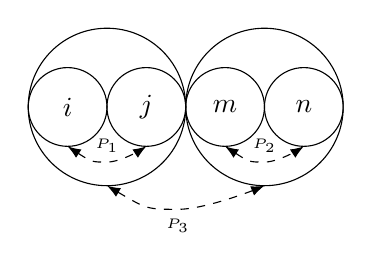
\begin{tikzpicture}[scale=1]
\coordinate (p1) at (2,5) {} {};
\coordinate (p2) at (3,5) {};
\coordinate (p3) at (4,5) {} {} {};
\coordinate (p4) at (5,5) {} {} {};
\coordinate (l1) at (2.5,5) {} {};
\coordinate (l2) at (4.5,5) {};
\draw  (p1) circle(0.5);
\node at (p1)  {$i$};
\draw  (p2) circle(0.5);
\node at (p2)  {$j$};
\draw  (p3) circle(0.5);
\node at (p3)  {$m$};
\draw  (p4) circle(0.5);
\node at (p4)  {$n$};
\draw  (l1) circle(1.);
\draw  (l2) circle(1.);



\draw [Latex-Latex ,dashed] plot[smooth, tension=.7] coordinates {(2,4.5) (2.5,4.3) (3,4.5)};
\draw   [Latex-Latex ,dashed]plot[smooth, tension=.7] coordinates {(4,4.5) (4.5,4.3) (5,4.5)};
\draw   [Latex-Latex ,dashed]plot[smooth, tension=.7] coordinates {(2.5,4) (3.4,3.7) (4.5,4)};
\node[anchor = south ] at (2.5,4.3)   {\tiny$P_1$};
\node[anchor = south ] at (4.5,4.3)  {\tiny$P_2$};
\node[anchor = north ] at (3.4,3.7)  {\tiny$P_3$};
\end{tikzpicture}}
\caption{Permutations}
\label{fig:fig_p247}
\end{figure}
The factor $\frac{1}{8}$ is explained by te fact that are $2^3$ possible permutations in the $i,j,m,n$ indexes i.e. $2\times2$ for the permutations $P_1$ and $P_2$ and again $2$ for the permutation $P_3$. Note that a single permutation $P_1$ or $P_2$ changes the sign of  $T_{ij}T_{mn}$ but also changes the sign of $\delta^{ijmn}_{1234}$, so the combined sign doesn't change. A double permutation $P_1$ and  $P_2$ changes the sign of  $T_{ij}$ and $T_{mn}$ resulting in a unchanged sign of  $T_{ij}T_{mn}$ but also $\delta^{ijmn}_{1234}$ is unchanged because of the double permutation. Finally $P_3$ has no effect, nor on $T_{ij}T_{mn}$ nor on $\delta^{ijmn}_{1234}$. So we have 8 repetitions for  the same set $i,j,m,n$.\\
So we have, 
\begin{align}
P&= \frac{1}{8}\delta^{ijmn}_{1234}T_{ij}T_{mn}\\
&= \frac{1}{8}\epsilon^{ijmn}T_{ij}T_{mn}
\end{align}
From this follows immediately as $\epsilon^{ijmn}$ is a relative tensor of weight $1$ and $T_{ij}$ an absolute tensor (i.e. a relative tensor of weight $0$) that $P$ is a relative tensor of eight $1$ i.e. a density.
$$\blacklozenge$$
\newpage



\section{p245 - Exercice }
\begin{tcolorbox}
Show that, for rectangular Cartesian coordinates, the vorticity tensor and the vorticity vector of a fluid are duals (cf. $\mathbf{6.130}$).
\end{tcolorbox}
$\mathbf{6.130}$:
\begin{align}
\omega_r=\half\epsilon_{rmn}\omega_{mn},\spatie \omega_{mn}=\epsilon_{rmn}\omega_r
\end{align}
Put $\hat{T}^r= \omega_r$ and $T_{mn} = \omega_{mn}$
then the expressions in $(1)$ can be expressed as (considering that the covariant an contravariant expressions are identical in rectangular Cartesian coordinates) 
\begin{align}
\hat{T}^r=\frac{1}{(3-2)!}\epsilon^{mnr}T_{mn},\spatie T_{mn}=\epsilon_{rmn}\hat{T}^r
\end{align}
which are exactly the general definitions $\mathbf{7.121}$ and $\mathbf{7.122}$ (with $N=3$ and $M=2$) for dual tensors.
$$\blacklozenge$$
\newpage



\section{p255 - Exercice }
\begin{tcolorbox}
Show that $\mathbf{7.305}$ may be written in the equivalent form
$$d\tau_{(M)}^{k_1\dots k_m}= \epsilon^{\beta_1\dots \beta_M}d_{(\beta_1)}x^{k_1}\dots d_{(\beta_M)}x^{k_M}$$
\end{tcolorbox}
The determinant of a matrix and its transpose are equal.\\
Hence we can rewrite $\mathbf{7.305} \quad \delta^{k_1\dots k_M}_{s_1\dots s_M}d_{(1)}x^{s_1}\dots d_{(M)}x^{s_M}$ as
\begin{align}
d\tau_{(M)}^{k_1\dots k_m}=\delta_{k_1\dots k_M}^{s_1\dots s_M}d_{(s_1)}x^{1}\dots d_{(s_M)}x^{M}
\end{align}
In order to be consistent with the notation we replace the $s_i$ by $\alpha_i$ as the summation occurs along the constants $c^{(i)}$
\begin{align}
d\tau_{(M)}^{k_1\dots k_m}=\delta_{k_1\dots k_M}^{\alpha_1\dots \alpha_M}d_{(\alpha_1)}x^{1}\dots d_{(\alpha_M)}x^{M}
\end{align}
Given the set $\{k_1, k_2,\dots , k_M\}$ we can represent the sequence $\{1,2,\dots , M\}$ by $\{k_j, k_m,\dots ,k_M,\dots k_n\}$ (imagine that $k_j=1, k_m=2,...$ etc.). We rewrite $(2)$ as
\begin{align}
d\tau_{(M)}^{k_1 k_2\dots k_m}=(\theta_{\alpha}) \delta_{1 2 \dots M}^{\alpha_1\dots \alpha_M}d_{(\alpha_1)}x^{k_j}d_{(\alpha_2)}x^{k_m}\dots d_{(\alpha_M)}x^{k_n}
\end{align}
where 
\begin{align}
\theta_{\alpha} = \epsilon_{k_1 k_2\dots k_M}
\end{align}
( a permutation in the lower indexes of the generalized Kronecker deltas symbol will invert the sign depending on the 'oddness' of the permutation).
Let's rearrange the product $d_{(\alpha_1)}x^{k_j}d_{(\alpha_2)}x^{k_m}\dots d_{(\alpha_M)}x^{k_n}$ so that the indexes $k_i$ are naturally ordered
\begin{align}
d\tau_{(M)}^{k_1 k_2\dots k_m}=(\theta_{\alpha}) \delta_{1 2 \dots M}^{\alpha_1\dots \alpha_M}d_{(\alpha_r)}x^{k_1}d_{(\alpha_n)}x^{k_2}\dots d_{(\alpha_1)}x^{k_n}\dots d_{(\alpha_s)}x^{k_M}
\end{align}
and changing the order in the upper indexes of the general Kroneckers delta's:
\begin{align}
d\tau_{(M)}^{k_1 k_2\dots k_m}=(\theta_{\alpha})(\theta_{k}) \delta_{1 2 \dots M}^{\alpha_r\alpha_n \dots \alpha_s}d_{(\alpha_r)}x^{k_1}d_{(\alpha_n)}x^{k_2}\dots d_{(\alpha_1)}x^{k_n}\dots d_{(\alpha_s)}x^{k_M}
\end{align}
where $\theta_{k}= \pm 1$ depending on the 'oddness' of the permutation needed to go from $\{\alpha_1\dots \alpha_M\}$ to $\{\alpha_r\alpha_n \dots \alpha_s\}$.\\
As we can see in figure $7.2$,  it's no hard to see that 
\begin{align}
\theta_{k}=\theta_{\alpha}
\end{align}
\begin{figure}[H]%
    \centering
    \subfloat[]{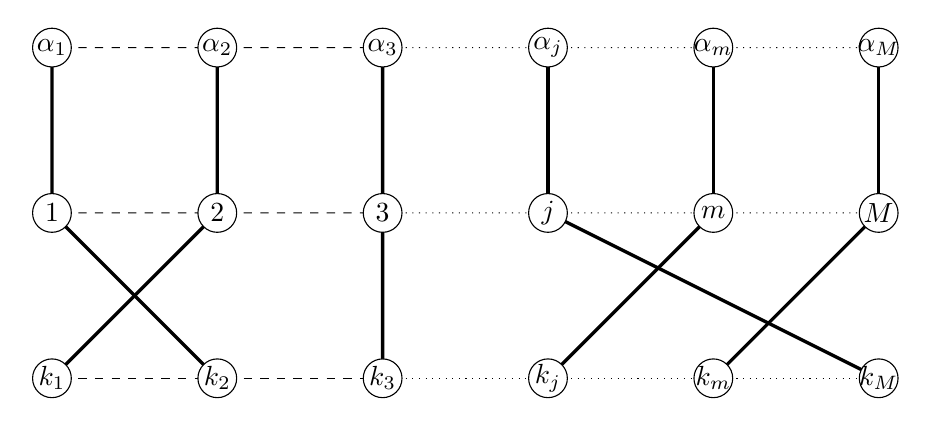
\begin{tikzpicture}[scale=0.7]


\node (alfa1) at (-10,6) {};
\node (alfaM) at (5,6) {};
\node (alfa2)at (-7,6) {};
\node (alfa3) at (-4,6) {};
\node (alfa4)at (-1,6) {};
\node (alfa5)at (2,6) {};

\node (v1) at (-10,3) {};
\node (vM) at (5,3) {};
\node (v2)at (-7,3) {};
\node (v3) at (-4,3) {};
\node (v4)at (-1,3) {};
\node (v5)at (2,3) {};

\node (k1) at (-10,0) {};
\node (kM) at (5,0) {};
\node (k2)at (-7,0) {};
\node (k3) at (-4,0) {};
\node (k4)at (-1,0) {};
\node (k5)at (2,0) {};


\draw[very thick]  (alfa1) --(v1);
\draw[very thick]  (alfa2) --(v2);
\draw[very thick]  (alfa3) --(v3);
\draw[very thick]  (alfa4) --(v4);
\draw[very thick]  (alfa5) --(v5);
\draw[very thick]  (alfaM) --(vM);
\draw[very thick]  (k2) --(v1);
\draw[very thick]  (k1) --(v2);
\draw[very thick]  (k3) --(v3);
\draw[very thick]  (kM) --(v4);
\draw[very thick]  (k4) --(v5);
\draw[very thick]  (k5) --(vM);



\draw[dashed]  (alfa1) --(alfa2);
\draw[dashed]  (alfa2) --(alfa3);
\draw[dotted]  (alfa3) --(alfa4);
\draw[dotted]  (alfa4) --(alfa5);
\draw [dotted](alfa5) --(alfaM);

\draw  [fill= white](alfa1)circle (10pt);
\draw  [fill= white](alfaM)circle (10pt);
\draw  [fill= white](alfa2)circle (10pt);
\draw  [fill= white](alfa3)circle (10pt);
\draw  [fill= white](alfa4)circle (10pt);
\draw  [fill= white](alfa5)circle (10pt);

\node[] at (alfa1)  {$\alpha_1$};
\node[] at (alfaM)  {$\alpha_M$};
\node[] at (alfa2)  {$\alpha_2$};
\node[] at (alfa3)  {$\alpha_3$};
\node[] at (alfa4)  {$\alpha_j$};
\node[] at (alfa5)  {$\alpha_m$};



\draw [dashed] (v1) --(v2);
\draw[dashed]  (v2) --(v3);
\draw[dotted]  (v3) --(v4);
\draw[dotted]  (v4) --(v5);

\draw  [dotted](v5) --(vM);
\draw  [fill= white](v1)circle (10pt);
\draw  [fill= white](vM)circle (10pt);
\draw  [fill= white](v2)circle (10pt);
\draw  [fill= white](v3)circle (10pt);
\draw  [fill= white](v4)circle (10pt);
\draw  [fill= white](v5)circle (10pt);

\node[] at (v1)  {$1$};
\node[] at (vM)  {$M$};
\node[] at (v2)  {$2$};
\node[] at (v3)  {$3$};
\node[] at (v4)  {$j$};
\node[] at (v5)  {$m$};



\draw[dashed]  (k1) --(k2);
\draw[dashed]  (k2) --(k3);
\draw[dotted]  (k3) --(k4);
\draw[dotted]  (k4) --(k5);

\draw  [dotted](k5) --(kM);
\draw  [fill= white](k1)circle (10pt);
\draw  [fill= white](kM)circle (10pt);
\draw  [fill= white](k2)circle (10pt);
\draw  [fill= white](k3)circle (10pt);
\draw  [fill= white](k4)circle (10pt);
\draw  [fill= white](k5)circle (10pt);

\node[] at (k1)  {$k_1$};
\node[] at (kM)  {$k_M$};
\node[] at (k2)  {$k_2$};
\node[] at (k3)  {$k_3$};
\node[] at (k4)  {$k_j$};
\node[] at (k5)  {$k_m$};


\end{tikzpicture}}\\
    \subfloat[]{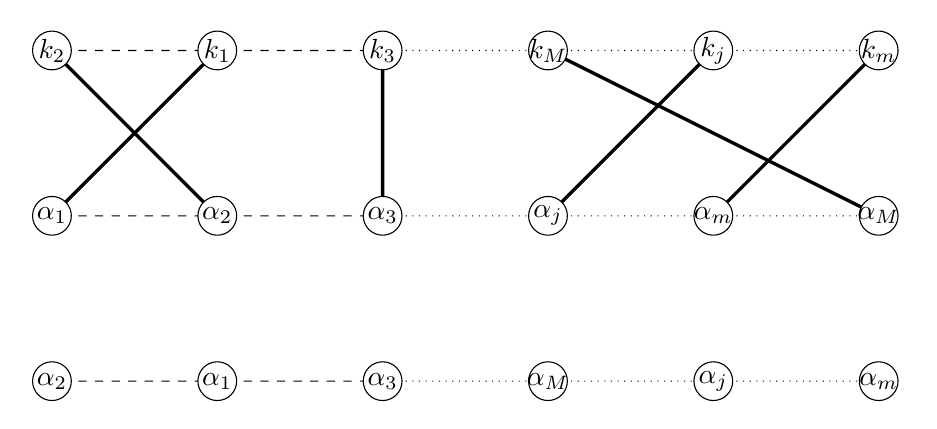
\begin{tikzpicture}[scale=0.7]


\node (alfaPR1) at (-10,-9) {};
\node (alfaPRM) at (5,-9) {};
\node (alfaPR2)at (-7,-9) {};
\node (alfaPR3) at (-4,-9) {};
\node (alfaPR4)at (-1,-9) {};
\node (alfaPR5)at (2,-9) {};

\node (alfaP1) at (-10,-6) {};
\node (alfaPM) at (5,-6) {};
\node (alfaP2)at (-7,-6) {};
\node (alfaP3) at (-4,-6) {};
\node (alfaP4)at (-1,-6) {};
\node (alfaP5)at (2,-6) {};

\node (kp1) at (-10,-3) {};
\node (kpM) at (5,-3) {};
\node (kp2)at (-7,-3) {};
\node (kp3) at (-4,-3) {};
\node (kp4)at (-1,-3) {};
\node (kp5)at (2,-3) {};



\draw[very thick]  (alfaP2) --(kp1);
\draw[very thick]  (alfaP1) --(kp2);
\draw[very thick]  (alfaP3) --(kp3);
\draw[very thick]  (alfaPM) --(kp4);
\draw[very thick]  (alfaP4) --(kp5);
\draw[very thick]  (alfaP5) --(kpM);



\draw [dashed] (kp1) --(kp2);
\draw [dashed] (kp2) --(kp3);
\draw[dotted]  (kp3) --(kp4);
\draw[dotted]  (kp4) --(kp5);
\draw  [dotted](kp5) --(kpM);

\draw  [fill= white](kp1)circle (10pt);
\draw  [fill= white](kpM)circle (10pt);
\draw  [fill= white](kp2)circle (10pt);
\draw  [fill= white](kp3)circle (10pt);
\draw  [fill= white](kp4)circle (10pt);
\draw  [fill= white](kp5)circle (10pt);

\node[] at (kp1)  {$k_2$};
\node[] at (kpM)  {$k_m$};
\node[] at (kp2)  {$k_1$};
\node[] at (kp3)  {$k_3$};
\node[] at (kp4)  {$k_M$};
\node[] at (kp5)  {$k_j$};

\draw[dashed]  (alfaP1) --(alfaP2);
\draw[dashed]  (alfaP2) --(alfaP3);
\draw[dotted]  (alfaP3) --(alfaP4);
\draw[dotted]  (alfaP4) --(alfaP5);
\draw [dotted](alfaP5) --(alfaPM);

\draw[dashed]  (alfaPR1) --(alfaPR2);
\draw[dashed]  (alfaPR2) --(alfaPR3);
\draw[dotted]  (alfaPR3) --(alfaPR4);
\draw[dotted]  (alfaPR4) --(alfaPR5);
\draw [dotted](alfaPR5) --(alfaPRM);

\draw  [fill= white](alfaP1)circle (10pt);
\draw  [fill= white](alfaPM)circle (10pt);
\draw  [fill= white](alfaP2)circle (10pt);
\draw  [fill= white](alfaP3)circle (10pt);
\draw  [fill= white](alfaP4)circle (10pt);
\draw  [fill= white](alfaP5)circle (10pt);

\draw  [fill= white](alfaPR1)circle (10pt);
\draw  [fill= white](alfaPRM)circle (10pt);
\draw  [fill= white](alfaPR2)circle (10pt);
\draw  [fill= white](alfaPR3)circle (10pt);
\draw  [fill= white](alfaPR4)circle (10pt);
\draw  [fill= white](alfaPR5)circle (10pt);

\node[] at (alfaP1)  {$\alpha_1$};
\node[] at (alfaPM)  {$\alpha_M$};
\node[] at (alfaP2)  {$\alpha_2$};
\node[] at (alfaP3)  {$\alpha_3$};
\node[] at (alfaP4)  {$\alpha_j$};
\node[] at (alfaP5)  {$\alpha_m$};

\node[] at (alfaPR1)  {$\alpha_2$};
\node[] at (alfaPRM)  {$\alpha_m$};
\node[] at (alfaPR2)  {$\alpha_1$};
\node[] at (alfaPR3)  {$\alpha_3$};
\node[] at (alfaPR4)  {$\alpha_M$};
\node[] at (alfaPR5)  {$\alpha_j$};
\end{tikzpicture}}
\caption{Permutations}
\label{fig:fig_p255}
\end{figure}
Indeed suppose, as in the example $(a)$ ,  $k_1=2, k_2=1,k_3=3, ,\dots ,k_j = m,\dots , k_m=j,\dots$ etc., so we get a sequence $\{k_2, k_1,k_3,\dots, k_m,\dots k_j,\dots\}$ as illustrated in $(b)$. But to have - with this sequence - an equivalent expression of 
$d\tau_{(M)}^{k_1 k_2\dots k_m}=(\theta_{\alpha}) \delta_{1 2 \dots M}^{\alpha_1\dots \alpha_M}d_{(\alpha_1)}x^{k_j}d_{(\alpha_2)}x^{k_m}\dots d_{(\alpha_M)}x^{k_n}$, we need to make an equivalent permutation so that $\alpha_r$ gets in the same position  as $k_r$, resulting in a new sequence $\{\alpha_2,\alpha_1,\alpha_3,\dots,\alpha_M,\dots,\alpha_j, \alpha_m\}$.\\
The number of permutations to generate $\theta_{\alpha}$ and $\theta_k$ are identical resulting in $\theta_{\alpha}\theta_k=1$.
So $(6)$ can be rewritten (noting that the $\alpha_r$ are dummy indexes and that we are free to rename them so that $r=1, n=2,\dots$) 
\begin{align}
d\tau_{(M)}^{k_1 k_2\dots k_m}= \delta_{1 2 \dots M}^{\beta_1\beta_2 \dots \beta_M}d_{(\beta_1)}x^{k_1}d_{(\beta_2)}x^{k_2}\dots d_{(\beta_n)}x^{k_n}\dots d_{(\beta_M)}x^{k_M}
\end{align}
Finally, using $\mathbf{7.114}$ 
\begin{align}
d\tau_{(M)}^{k_1 k_2\dots k_m}&= \underbrace{\epsilon_{1 2 \dots M}}_{=1}\epsilon^{\beta_1\beta_2 \dots \beta_M}d_{(\beta_1)}x^{k_1}d_{(\beta_2)}x^{k_2}\dots d_{(\beta_n)}x^{k_n}\dots d_{(\beta_M)}x^{k_M}\\
&= \epsilon^{\beta_1\beta_2 \dots \beta_M}d_{(\beta_1)}x^{k_1}d_{(\beta_2)}x^{k_2}\dots d_{(\beta_n)}x^{k_n}\dots d_{(\beta_M)}x^{k_M}
\end{align}
$$\blacklozenge$$
\newpage


\section{p257 - Exercice }
\begin{tcolorbox}
Let $x^k$ be rectangular Cartesian coordinates in Euclidean $3-$space. Introduce polar coordinates $r,\theta,\phi$ and consider the surface of the sphere $r=a$. On this sphere form the infinitesimal $2-$cell with corners $(\theta,\phi),\ (\theta+d\theta,\phi),\ (\theta,\phi+d\phi),\ (\theta+d\theta,\phi+d\phi)$. Determine the extension of this cell and interpret the rectangular components. In particular, show that the three independent components of the extension are (apart from the sign) equal to the areas obtained by normal projection of the cell onto the three rectangular planes. Does this interpretation remain valid if the sphere is replaces by some other surface?
\end{tcolorbox}
We use $\mathbf{7.312}$:
\begin{align}
d\tau_{(2)}^{k_1k_2}&= \epsilon^{\alpha_1\alpha_2}\pdv{x^{k_1}}{y^{\alpha_1}}\pdv{x^{k_2}}{y^{\alpha_2}}\left|d_{(\beta)}y^{\gamma}\right|
\end{align}
with $(y^1, y^2)= (\theta,\phi)$ giving if we take $f^{(i)}=c^{(i)} $ as $\theta=c^{(1)},\ \phi =c^{(2)} $:
\begin{align}
\left|d_{(\beta)}y^{\gamma}\right|&=\left|\begin{matrix}d_{(1)}y^{1}&d_{(1)}y^{2}\\
d_{(2)}y^{1}&d_{(2)}y^{2}\end{matrix}\right|\\
&=\left|\begin{matrix}d{\theta}&0\\
0&d{\phi}\end{matrix}\right|\\
&= d{\theta}d{\phi}
\end{align}
We also have
\begin{align}
\left\{\begin{array}{l}
x= a\sin{\theta}\cos{\phi}\\
y= a\sin{\theta}\sin{\phi}\\
z= a\cos{\theta}\\
\end{array}\right.\\
\end{align}
giving
\begin{align}
\left\{\begin{array}{l}
\pdv{x}{\theta}= a\cos{\theta}\cos{\phi}\\
\pdv{x}{\phi}= -a\sin{\theta}\sin{\phi}\\
\pdv{y}{\theta}= a\cos{\theta}\sin{\phi}\\
\pdv{y}{\phi}=  a\sin{\theta}\cos{\phi}\\
\pdv{z}{\theta}= -a\sin{\theta}\\
\pdv{z}{\phi}= 0\\
\end{array}\right.\\
\end{align}

and get 
\begin{align}
d\tau_{(2)}^{xy}&= \underbrace{\epsilon^{11}}_{=0}\pdv{x}{\theta}\pdv{y}{\theta}d{\theta}d{\phi}+\epsilon^{12}\pdv{x}{\theta}\pdv{y}{\phi}d{\theta}d{\phi}+\epsilon^{21}\pdv{x}{\phi}\pdv{y}{\theta}d{\theta}d{\phi}+\underbrace{\epsilon^{22}}_{=0}\pdv{x}{\phi}\pdv{y}{\phi}d{\theta}d{\phi}\\
&=a^2\cos{\theta}\cos{\phi}\sin{\theta}\cos{\phi}d{\theta}d{\phi}
+a^2\sin{\theta}\sin{\phi}\cos{\theta}\sin{\phi}d{\theta}d{\phi}\\
&=a^2\cos{\theta}\sin{\theta}d{\theta}d{\phi}\\
d\tau_{(2)}^{yx}&=-a^2\cos{\theta}\sin{\theta}d{\theta}d{\phi}
\end{align}
\begin{align}
d\tau_{(2)}^{xz}&= \underbrace{\epsilon^{11}}_{=0}\pdv{x}{\theta}\pdv{z}{\theta}d{\theta}d{\phi}+\epsilon^{12}\pdv{x}{\theta}\underbrace{\pdv{z}{\phi}}_{=0}d{\theta}d{\phi}+\epsilon^{21}\pdv{x}{\phi}\pdv{z}{\theta}d{\theta}d{\phi}+\underbrace{\epsilon^{22}}_{=0}\pdv{x}{\phi}\pdv{z}{\phi}d{\theta}d{\phi}\\
&=-a^2\sin^2{\theta}\sin{\phi}d{\theta}d{\phi}\\
d\tau_{(2)}^{zx}&=a^2\sin^2{\theta}\sin{\phi}d{\theta}d{\phi}
\end{align}
\begin{align}
d\tau_{(2)}^{yz}&= \underbrace{\epsilon^{11}}_{=0}\pdv{y}{\theta}\pdv{z}{\theta}d{\theta}d{\phi}+\epsilon^{12}\pdv{y}{\theta}\underbrace{\pdv{z}{\phi}}_{=0}d{\theta}d{\phi}+\epsilon^{21}\pdv{y}{\phi}\pdv{z}{\theta}d{\theta}d{\phi}+\underbrace{\epsilon^{22}}_{=0}\pdv{y}{\phi}\pdv{z}{\phi}d{\theta}d{\phi}\\
&=a^2\sin^2{\theta}\cos{\phi}d{\theta}d{\phi}\\
d\tau_{(2)}^{zy}&=-a^2\sin^2{\theta}\cos{\phi}d{\theta}d{\phi}
\end{align}
\begin{align}
d\tau_{(2)}^{xx}&= \underbrace{\epsilon^{11}}_{=0}\pdv{x}{\theta}\pdv{x}{\theta}d{\theta}d{\phi}+\epsilon^{12}\pdv{x}{\theta}\pdv{x}{\phi}d{\theta}d{\phi}+\epsilon^{21}\pdv{x}{\phi}\pdv{x}{\theta}d{\theta}d{\phi}+\underbrace{\epsilon^{22}}_{=0}\pdv{x}{\phi}\pdv{x}{\phi}d{\theta}d{\phi}\\
&=0
\end{align}

\begin{align}
d\tau_{(2)}^{yy}&= \underbrace{\epsilon^{11}}_{=0}\pdv{y}{\theta}\pdv{y}{\theta}d{\theta}d{\phi}+\epsilon^{12}\pdv{y}{\theta}\pdv{y}{\phi}d{\theta}d{\phi}+\epsilon^{21}\pdv{y}{\phi}\pdv{y}{\theta}d{\theta}d{\phi}+\underbrace{\epsilon^{22}}_{=0}\pdv{y}{\phi}\pdv{y}{\phi}d{\theta}d{\phi}\\
&=0
\end{align}

\begin{align}
d\tau_{(2)}^{zz}&= \underbrace{\epsilon^{11}}_{=0}\pdv{z}{\theta}\pdv{z}{\theta}d{\theta}d{\phi}+\epsilon^{12}\pdv{z}{\theta}\underbrace{\pdv{z}{\phi}}_{=0}d{\theta}d{\phi}+\epsilon^{21}\underbrace{\pdv{z}{\phi}}_{=0}\pdv{z}{\theta}d{\theta}d{\phi}+\underbrace{\epsilon^{22}}_{=0}\pdv{z}{\phi}\pdv{z}{\phi}d{\theta}d{\phi}\\
&=0
\end{align}
\begin{figure}[H]%
    \centering
    \subfloat[]{
%Axis Angles  
\tdplotsetmaincoords{70}{110}

%Macros  
\pgfmathsetmacro{\rvec}{7.5}  
\pgfmathsetmacro{\thetavec}{40}  
\pgfmathsetmacro{\phivec}{45}

\pgfmathsetmacro{\dphivec}{20}  
\pgfmathsetmacro{\dthetavec}{20}  

%Layers  
\pgfdeclarelayer{background} 
\pgfdeclarelayer{foreground}

\pgfsetlayers{background, main, foreground}
\begin{tikzpicture}
	[scale=0.8,
		tdplot_main_coords,
		axis/.style={->,black,thick},
		vector/.style={-stealth,black, thick},
		vector guide/.style={dashed,black,thick},
		angle/.style={black,thick}]

	%standard tikz coordinate definition using x, y, z coords
	\coordinate (O) at (0,0,0);

\tdplotsetcoord{E}{\rvec }{\thetavec}{\phivec}  
\tdplotsetcoord{F}{\rvec }{\thetavec + \dthetavec}{\phivec}  
\tdplotsetcoord{F'}{\rvec }{90}{\phivec}  \tdplotsetcoord{G}{\rvec }{\thetavec + \dthetavec}{\phivec + \dphivec}  
\tdplotsetcoord{G'}{\rvec }{90}{\phivec + \dphivec} 
\tdplotsetcoord{H}{\rvec }{\thetavec}{\phivec + \dphivec} 
    
%Axis  
\begin{pgfonlayer}{background}  
    \draw[thick,-latex] (0,0,0) -- (7,0,0) node[pos=1.1]{$x$};        
    \draw[thick,-latex] (0,0,0) -- (0,7,0) node[pos=1.05]{$y$};         
    \draw[thick,-latex] (0,0,0) -- (0,0,6) node[pos=1.05]{$z$};                   
\end{pgfonlayer}

%Help Lines  
\begin{pgfonlayer}{background}  
    %Up     
      
   
  
    %Down   
    \draw[dashed] (O) -- (F');  
    \draw[dashed] (O) -- (G');  
\end{pgfonlayer}  
\begin{pgfonlayer}{foreground}  
    %%Help Curves   
    \tdplotsetthetaplanecoords{\phivec}     
    %
    \tdplotdrawarc[dotted,tdplot_rotated_coords]{(O)}{\rvec}{\thetavec+\dthetavec}{90}{}{}
    %
    \tdplotsetthetaplanecoords{\phivec+\dphivec}    
    \tdplotdrawarc[dotted,tdplot_rotated_coords]{(O)}{\rvec}{\thetavec+\dthetavec}{90}{}{}

    %    
    \tdplotdrawarc[dotted,tdplot_main_coords]{(O)}{\rvec}{\phivec}{\phivec+\dphivec}{below, rotate=13}{} 
\end{pgfonlayer}


%Angles  
\begin{pgfonlayer}{foreground}  
    %Phi, dPhi  
    \tdplotdrawarc[-stealth]{(O)}{0.9}{0}{\phivec}{anchor=north}{$\phi$}    
    \tdplotdrawarc[-stealth]{(O)}{1.5}{\phivec}{\phivec + \dphivec}{}{} 
    \node at (1.4,1.9,0) {$\mathrm{d}\phi$};        
    \tdplotsetthetaplanecoords{\phivec}     
    %Theta, dTheta          
    \tdplotdrawarc[tdplot_rotated_coords,-stealth]{(0,0,0)}{1.2}{0}{\thetavec}{}{}      
    \node at (0,0.3,1.3) {$\theta$};    
    \tdplotdrawarc[tdplot_rotated_coords,-stealth]{(0,0,0)}{2.5}{\thetavec}{\thetavec + \dthetavec}{anchor=south west}{$\mathrm{d}\theta$}  
\end{pgfonlayer}

%Differential Volume

%%Lines  
\begin{pgfonlayer}{foreground}  
    \draw[dashed] (O) -- (E) node[midway, above left]{a};    
    \draw[dashed] (O) -- (F);    
    \draw[dashed] (O) -- (G);      
\end{pgfonlayer}   
\begin{pgfonlayer}{background}
    \draw[dashed] (O) -- (H);  
\end{pgfonlayer}

%%Curved 

 \begin{pgfonlayer}{foreground}     
    \tdplotsetthetaplanecoords{\phivec}       
    \tdplotdrawarc[tdplot_rotated_coords, thick]{(O)}{\rvec }{\thetavec}{\dthetavec + \thetavec}{}{}
    %   
    \tdplotsetthetaplanecoords{\phivec + \dphivec}  
    \tdplotdrawarc[tdplot_rotated_coords, thick]{(O)}{\rvec }{\thetavec}{\dthetavec + \thetavec}{above right}{$a\mathrm{d}\theta$}  
    %   
    \tdplotsetrotatedcoords{55}{-50.4313}{-6.4086}  
    \tdplotdrawarc[tdplot_rotated_coords, thick]{(O)}{\rvec }{0}{12.8173}{anchor=south }{$a\sin\theta\mathrm{d}\phi$}      
    %   
    \tdplotsetrotatedcoords{55}{-30.3813}{-8.6492}          
    \tdplotdrawarc[tdplot_rotated_coords, thick]{(O)}{\rvec}{0}{17.2983}{}{}  
\end{pgfonlayer}

%Fill Color 
\begin{pgfonlayer}{main}    
    %Front  
    \fill[gray, opacity=0.2] (E) to[bend left=4] (F)  to[bend left=2] (G) to[bend right=6.5] (H) to[bend right=4] cycle;   
\end{pgfonlayer}  

%\node at (E) {E};
%\node at (F) {F};
%\node at (G) {G};
%\node at (H) {H};
\end{tikzpicture}
}\\
    \subfloat[]{
%Axis Angles  
\tdplotsetmaincoords{75}{120}
%\tdplotsetmaincoords{90}{0}

%Macros  
\pgfmathsetmacro{\rvec}{7.5}  
\pgfmathsetmacro{\thetavec}{60}  
\pgfmathsetmacro{\phivec}{60}

\pgfmathsetmacro{\dphivec}{20}  
\pgfmathsetmacro{\dthetavec}{10}  

%Layers  
\pgfdeclarelayer{background} 
\pgfdeclarelayer{foreground}

\pgfsetlayers{background, main, foreground}
\begin{tikzpicture}
	[scale=1,
		tdplot_main_coords,
		axis/.style={->,black,thick},
		vector/.style={-stealth,black, thick},
		vector guide/.style={dashed,black,thick},
		angle/.style={black,thick}]

	%standard tikz coordinate definition using x, y, z coords
	\coordinate (O) at (0,0,0);

\tdplotsetcoord{E}{\rvec }{\thetavec}{\phivec}  
\tdplotsetcoord{F}{\rvec }{\thetavec + \dthetavec}{\phivec}  
\tdplotsetcoord{F'}{\rvec/3 }{90}{\phivec}  
\tdplotsetcoord{G}{\rvec }{\thetavec + \dthetavec}{\phivec + \dphivec}  
\tdplotsetcoord{G'}{\rvec /3}{90}{\phivec + \dphivec} 
\tdplotsetcoord{H}{\rvec }{\thetavec}{\phivec + \dphivec} 

%\coordinate (E") at {0,\rvec*sin(\phivec )*cos(\thetavec ),100*\rvec*cos(\phivec )};
\draw[dotted] (E) -- (Exz); 
\draw[dotted] (H) -- (Hxz) ;
\draw[dotted] (F) -- (Fxz) ;
\draw[dotted] (G) -- (Gxz) ;
\draw[thick] (Exz) -- (Hxz)-- (Gxz)-- (Fxz) -- cycle;
\draw[thick] (E) -- (H)-- (G)-- (F) -- cycle;


\draw [fill=white](E)circle (1.5pt);
    
%Axis  
\begin{pgfonlayer}{background}  
    \draw[thick,-latex] (0,0,0) -- (5,0,0) node[pos=1.1]{$x$};        
    \draw[thick,-latex] (0,0,0) -- (0,6,0) node[pos=1.05]{$y$};         
    \draw[thick,-latex] (0,0,0) -- (0,0,4.5) node[pos=1.05]{$z$};                   
\end{pgfonlayer}

%Help Lines  
\begin{pgfonlayer}{background}  
    %Up     
      
   
  
    %Down   
    \draw[dashed,ultra thin](O) -- (F');  
    \draw[dashed,ultra thin] (O) -- (G');  
\end{pgfonlayer}  

%Angles  
\begin{pgfonlayer}{foreground}  
    %Phi, dPhi  
    \tdplotdrawarc[-stealth]{(O)}{0.9}{0}{\phivec}{anchor=north}{$\phi$}    
    \tdplotdrawarc[-stealth]{(O)}{1.5}{\phivec}{\phivec + \dphivec}{}{} 
    \node at (1.4,1.9,0) {$\mathrm{d}\phi$};        
    \tdplotsetthetaplanecoords{\phivec}     
    %Theta, dTheta          
    \tdplotdrawarc[tdplot_rotated_coords,-stealth]{(0,0,0)}{1.2}{0}{\thetavec}{}{}      
    \node at (0,0.3,1.3) {$\theta$};    
    \tdplotdrawarc[tdplot_rotated_coords,-stealth]{(0,0,0)}{2.5}{\thetavec}{\thetavec + \dthetavec}{anchor=south west}{$\mathrm{d}\theta$}  
\end{pgfonlayer}

%Differential Volume

%%Lines  
\begin{pgfonlayer}{foreground}  
    \draw[dashed,ultra thin] (O) -- (E) ;%node[midway, above left]{a};    
    \draw[dashed,ultra thin](O) -- (F);    
    \draw[dashed,ultra thin](O) -- (G);      
\end{pgfonlayer}   
\begin{pgfonlayer}{background}
   \draw[dashed,ultra thin] (O) -- (H);  
\end{pgfonlayer}

%%Curved 



%Fill Color 
\begin{pgfonlayer}{main}    
    %Front  
    \fill[gray, opacity=0.2] (E) to[bend left=4] (F)  to[bend left=2] (G) to[bend right=6.5] (H) to[bend right=4] cycle;  
\fill[gray, opacity=0.2] (Exz) to[bend left=4] (Fxz)  to[bend left=2] (Gxz) to[bend right=6.5] (Hxz) to[bend right=4] cycle;      
\end{pgfonlayer}  


\node[anchor=north west] at (H) {$\quad ad\theta$};
\node[anchor=north west] at (F) {$\quad a\sin{\theta}d\phi$};
\node[anchor=south east] at (Gxz) {$ a\sin{\theta}d\theta \quad\quad \quad$};
\node[anchor=south ] at (Exz) {$a\sin{\theta}\sin{\phi}d\phi \quad\quad \quad \quad$};
\begin{pgfonlayer}{foreground}  
    %\draw[dashdotted, thick] (E) -- (Exy) ;  
    %\draw[dashdotted,thick] (E) -- (Eyz) ;  
\end{pgfonlayer} 

  

\coordinate (P) at (2.5,5.2,-0.12);
\draw [fill=white](P)circle (1.5pt);

\coordinate (P') at (2.8,6.2,-0.18);
\draw [fill=white](P')circle (1.5pt);
\draw[dashdotted,thick] (F) -- (P'); 
\draw[dashdotted,thick] (E) -- (P); 
%Angles  
\begin{pgfonlayer}{foreground}  
    %Phi, dPhi  
\tdplotsetthetaplanecoords{\thetavec} 
    \tdplotdrawarc[tdplot_rotated_coords,-stealth]{(E)}{-3.65}{1}{-24}{}{};          
\node[anchor=north east] at (P'){$\frac{\pi}{2}-\theta$};
\end{pgfonlayer}

\coordinate (Q) at (Eyz);
\draw [fill=white](Q)circle (1.5pt);

\coordinate (Q') at (0,6.7,3.73);
\draw [fill=white](Q')circle (1.5pt);
\draw[dashdotted,thick] (E) -- (Q); 
\draw[dashdotted,thick] (H) -- (Q'); 
%Angles  
\begin{pgfonlayer}{foreground}  
    %Phi, dPhi  
\tdplotsetthetaplanecoords{\thetavec} ;
    \tdplotdrawarc[-stealth]{(E)}{-3.4}{1}{-17}{}{};          
\node[anchor=south west] at (Q){$\quad\quad \frac{\pi}{2}-\phi$};
\end{pgfonlayer}
\end{tikzpicture}
}\\
    \subfloat[]{
\tdplotsetmaincoords{75}{120}
%\tdplotsetmaincoords{90}{0}

%Macros  
\pgfmathsetmacro{\rvec}{7.5}  
\pgfmathsetmacro{\thetavec}{60}  
\pgfmathsetmacro{\phivec}{60}

\pgfmathsetmacro{\dphivec}{20}  
\pgfmathsetmacro{\dthetavec}{10}  

%Layers  
\pgfdeclarelayer{background} 
\pgfdeclarelayer{foreground}

\pgfsetlayers{background, main, foreground}
\begin{tikzpicture}
	[scale=1,
		tdplot_main_coords,
		axis/.style={->,black,thick},
		vector/.style={-stealth,black, thick},
		vector guide/.style={dashed,black,thick},
		angle/.style={black,thick}]

	%standard tikz coordinate definition using x, y, z coords
	\coordinate (O) at (0,0,0);

\tdplotsetcoord{E}{\rvec }{\thetavec}{\phivec}  
\tdplotsetcoord{F}{\rvec }{\thetavec + \dthetavec}{\phivec}  
\tdplotsetcoord{F'}{\rvec/3 }{90}{\phivec}  
\tdplotsetcoord{G}{\rvec }{\thetavec + \dthetavec}{\phivec + \dphivec}  
\tdplotsetcoord{G'}{\rvec /3}{90}{\phivec + \dphivec} 
\tdplotsetcoord{H}{\rvec }{\thetavec}{\phivec + \dphivec} 

%\coordinate (E") at {0,\rvec*sin(\phivec )*cos(\thetavec ),100*\rvec*cos(\phivec )};
\draw[dotted] (E) -- (Exy); 
\draw[dotted] (H) -- (Hxy) ;
\draw[dotted] (F) -- (Fxy) ;
\draw[dotted] (G) -- (Gxy) ;
\draw[thick] (Exy) -- (Hxy)-- (Gxy)-- (Fxy) -- cycle;
\draw[thick] (E) -- (H)-- (G)-- (F) -- cycle;


\draw [fill=white](E)circle (1.5pt);
    
%Axis  
\begin{pgfonlayer}{background}  
    \draw[thick,-latex] (0,0,0) -- (5,0,0) node[pos=1.1]{$x$};        
    \draw[thick,-latex] (0,0,0) -- (0,9,0) node[pos=1.05]{$y$};         
    \draw[thick,-latex] (0,0,0) -- (0,0,4.5) node[pos=1.05]{$z$};                   
\end{pgfonlayer}

%Help Lines  
\begin{pgfonlayer}{background}  
    %Up     
      
   
  
    %Down   
    \draw[dashed,ultra thin](O) -- (F');  
    \draw[dashed,ultra thin] (O) -- (G');  
\end{pgfonlayer}  

%Angles  
\begin{pgfonlayer}{foreground}  
    %Phi, dPhi  
    \tdplotdrawarc[-stealth]{(O)}{0.9}{0}{\phivec}{anchor=north}{$\phi$}    
    \tdplotdrawarc[-stealth]{(O)}{1.5}{\phivec}{\phivec + \dphivec}{}{} 
    \node at (1.4,1.9,0) {$\mathrm{d}\phi$};        
    \tdplotsetthetaplanecoords{\phivec}     
    %Theta, dTheta          
    \tdplotdrawarc[tdplot_rotated_coords,-stealth]{(0,0,0)}{1.2}{0}{\thetavec}{}{}      
    \node at (0,0.3,1.3) {$\theta$};    
    \tdplotdrawarc[tdplot_rotated_coords,-stealth]{(0,0,0)}{2.5}{\thetavec}{\thetavec + \dthetavec}{anchor=south west}{$\mathrm{d}\theta$}  
\end{pgfonlayer}

%Differential Volume

%%Lines  
\begin{pgfonlayer}{foreground}  
    \draw[dashed,ultra thin] (O) -- (E) ;%node[midway, above left]{a};    
    \draw[dashed,ultra thin](O) -- (F);    
    \draw[dashed,ultra thin](O) -- (G);      
\end{pgfonlayer}   
\begin{pgfonlayer}{background}
   \draw[dashed,ultra thin] (O) -- (H);  
\end{pgfonlayer}

%%Curved 



%Fill Color 
\begin{pgfonlayer}{main}    
    %Front  
    \fill[gray, opacity=0.2] (E) to[bend left=4] (F)  to[bend left=2] (G) to[bend right=6.5] (H) to[bend right=4] cycle;  
\fill[gray, opacity=0.2] (Exy) to[bend left=4] (Fxy)  to[bend left=2] (Gxy) to[bend right=6.5] (Hxy) to[bend right=4] cycle;      
\end{pgfonlayer}  


\node[anchor=north west] at (H) {$\quad ad\theta$};
\node[anchor=north west] at (F) {$\quad a\sin{\theta}d\phi$};
\node[anchor=north east] at (Exy) {$ a\cos{\theta}d\theta $};
\node[anchor=north west] at (Fxy) {$ \quad \quad a\sin{\phi}d\phi $};
\begin{pgfonlayer}{foreground}  
    %\draw[dashdotted, thick] (E) -- (Exy) ;  
    %\draw[dashdotted,thick] (E) -- (Eyz) ;  
\end{pgfonlayer} 

  

\coordinate (P) at (2.5,5.2,-0.18);
\draw [fill=white](P)circle (1.5pt);

\coordinate (P') at (2.8,6.2,-0.18);
\draw [fill=white](P')circle (1.5pt);
\draw[dashdotted,thick] (F) -- (P'); 
\draw[dashdotted,thick] (E) -- (P); 
%Angles  
\begin{pgfonlayer}{foreground}  
    %Phi, dPhi  
\tdplotsetthetaplanecoords{\thetavec} 
    \tdplotdrawarc[tdplot_rotated_coords,-stealth]{(E)}{-1.25}{1}{-24}{}{};          
\node[anchor=north east] at (F){$\quad \quad \quad \frac{\pi}{2}-\theta$};
\end{pgfonlayer}


\end{tikzpicture}
}
\caption{Projections of extensions}
\label{fig:fig_p257}
\end{figure}
The quantities $d\tau_{(2)}^{xy},\ d\tau_{(2)}^{xz},  \ d\tau_{(2)}^{yz}$ are the projections of the extension on the respective Cartesian coordinates planes as can be seen in figure $7.3$ where figure $(a)$ depicts the extension (area = $a^2\sin{\theta}d\theta d\phi$) when choosing $\theta,\phi$ as the parameters $y^k$, while figure $(b)$ represents the projection of this extension on the $xz-$plane and figure $(c)$ represents the projection of this extension on the $xy-$plane.$$\lozenge$$ \\\\
\textbf{Does this interpretation remain valid if the sphere is replaces by some other surface?}
\\
The answer is no. For a two-space in Cartesian coordinates system  and with surface with parameters $(u,v)$, equation $(2)$ reduces to 
\begin{align}
d\tau_{(2)}^{xy}&= \left(\pdv{x}{u}\pdv{y}{v}-\pdv{x}{v}\pdv{y}{u}\right)dudv
\end{align}
So $d\tau_{(2)}^{xy}=0$ if $\pdv{x}{u}\pdv{y}{v}-\pdv{x}{v}\pdv{y}{u}=0$.
Consider the disk defined by the following parametric function
$$S: \left\{\mathbb{R}^2\rightarrow \mathbb{R}^3, \ S(u,v)= \left(\frac{u}{\sqrt{u^2+v^2+C}},\ \frac{v}{\sqrt{u^2+v^2+C}}, \ 1\right)\right\}$$ 
(the constant $C$ is there just to avoid the undefinedness of the surface for $(u,v) = (0,0)$). \\
It is easy to see that $\pdv{x}{u}\pdv{y}{v}-\pdv{x}{v}\pdv{y}{u}=0$, yet the surface is parallel with the $xy-$plane, which implies that the projection on the $xy-$plane of an elementary cell on $S$ will not have a zero area as can be seen in the figure hereunder. 

\begin{figure}[H]%
    \centering
    \pgfplotsset{every axis/.append style={
view={120}{20},
%axis equal image,
    %clip=false,
    %xlabel=$x$, ylabel=$y$, zlabel=$z$,
    %axis lines=middle,
    colormap={whitered}{
        color(0cm)=(white);
        color(1cm)=(black!75!gray)
    }
    %y dir=reverse,
%    axis on top
            }}
            


            
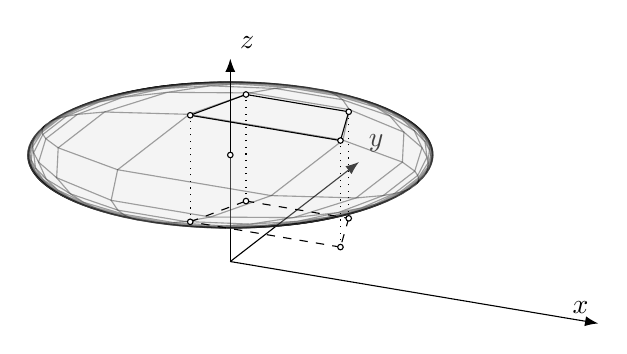
\begin{tikzpicture}[angle/.style={black,thick}]
\tikzmath{\a=0.05/sqrt(0.05*0.05+0.1*0.1);\k=1;\f=1;\u1=0;\v1=0;\u2=0;\v2=0;\u3=0;\v3=0;\u4=0;\v4=0;};
\a, \k,\u1,\v1,\u2,\v2,\u3,\v3,\u4,\v4,\f;
    %\pgfplotsset{ticks=none};
    \pgfplotsset{compat=1.12};
    \tikzset{>=latex} % for LaTeX arrow head
\begin{axis}
		[
		hide axis,clip=false,
		zmin=\k*0.5,
		zmax=\k,
			xmin=-\k,
		xmax=\k,
			ymin=-\k,
		ymax=\k,
		]
				%relevant points
	\coordinate (O) at ({ 0},{0},{0});%origin
	\coordinate (X) at ({ 2},{0},{0});%origin
	\coordinate (Y) at ({ 0},{1.5},{0});%origin
	\coordinate (Z) at ({ 0},{0},{0.4});%origin
	\coordinate (Q) at ({ 0},{0},{0.21});
	\draw[-Latex](O)--(X);
	\draw[-Latex](O)--(Y);
	\draw[](Q)--(O);
	\node[{anchor=south east}] at (X){$x$};
	\node[{anchor=south west}] at (Y){$y$};
	\node[{anchor=south west}] at (Z){$z$};
	\addplot3[surf,fill=gray!30,domain=-15:15,domain y=-15:15,samples=30,faceted color=black,mark=none, opacity=0.21,fill opacity = 0.3,thin]({x/sqrt(x*x*1+y*y+\f)},{y*\f/sqrt(x*x*1+y*y+\f)},{0.21});

\draw[-Latex](Q)--(Z);
\draw[fill=white](Q) circle(1pt)node[{anchor=north west}]{$$};; 	


	\tikzmath{\u1=0.5/sqrt(0.5*0.5+0.5*0.5+\f); \v1=0.5/sqrt(0.5*0.5+0.5*0.5+\f); 	};
	\coordinate (P0) at ({\u1},{\v1},{0.21});%origin
	\tikzmath{\u2=-0.5/sqrt(0.5*0.5+0.5*0.5+\f); \v2=0.5/sqrt(0.5*0.5+0.5*0.5+\f); 	};
	\coordinate (P1)at ({\u2},{\v2},{0.21});%origin
	\tikzmath{\u3=-0.5/sqrt(0.5*0.5+1.4*1.4+\f); \v3=1.4/sqrt(0.5*0.5+1.4*1.4+\f); 	};
	\coordinate (P2)at ({\u3},{\v3},{0.21});%origin
	\tikzmath{\u4=0.5/sqrt(0.5*0.5+1.4*1.4+\f); \v4=1.4/sqrt(0.5*0.5+1.4*1.4+\f); 	};
	\coordinate (P3)at ({\u4},{\v4},{0.21});%origin
	
		\coordinate (P0xy) at ({\u1},{\v1},{0});%origin
	\tikzmath{\u2=-0.5/sqrt(0.5*0.5+0.5*0.5+\f); \v2=0.5/sqrt(0.5*0.5+0.5*0.5+\f); 	};
	\coordinate (P1xy)at ({\u2},{\v2},{0});%origin
	\tikzmath{\u3=-0.5/sqrt(0.5*0.5+1.4*1.4+\f); \v3=1.4/sqrt(0.5*0.5+1.4*1.4+\f); 	};
	\coordinate (P2xy)at ({\u3},{\v3},{0});%origin
	\tikzmath{\u4=0.5/sqrt(0.5*0.5+1.4*1.4+\f); \v4=1.4/sqrt(0.5*0.5+1.4*1.4+\f); 	};
	\coordinate (P3xy)at ({\u4},{\v4},{0});%origin

	\draw[](P0)--(P1);
	\draw[](P1)--(P2);
	\draw[](P2)--(P3);
	\draw[](P3)--(P0);
	
	\draw[dashed](P0xy)--(P1xy);
	\draw[dashed](P1xy)--(P2xy);
	\draw[dashed](P2xy)--(P3xy);
	\draw[dashed](P3xy)--(P0xy);
	
	\draw[dotted](P0xy)--(P0);
	\draw[dotted](P1xy)--(P1);
	\draw[dotted](P2xy)--(P2);
	\draw[dotted](P3xy)--(P3);
	\draw[fill=white](P0) circle(1pt)node[{anchor=north west}]{$$};;
	\draw[fill=white](P1) circle(1pt)node[{anchor=north west}]{$$};;
	\draw[fill=white](P2) circle(1pt)node[{anchor=north west}]{$$};;
	\draw[fill=white](P3) circle(1pt)node[{anchor=north west}]{$$};;
	\draw[fill=white](P0xy) circle(1pt)node[{anchor=north west}]{$$};;
	\draw[fill=white](P1xy) circle(1pt)node[{anchor=north west}]{$$};;
	\draw[fill=white](P2xy) circle(1pt)node[{anchor=north west}]{$$};;
	\draw[fill=white](P3xy) circle(1pt)node[{anchor=north west}]{$$};;
	
\end{axis}
\end{tikzpicture}
\caption{A disk defined as $S: \left\{\mathbb{R}^2\rightarrow \mathbb{R}^3, \ S(u,v)= \left(\frac{u}{\sqrt{u^2+v^2+C}},\ \frac{v}{\sqrt{u^2+v^2+C}}, \ 1\right)\right\}$}
\label{fig:fig_p257}
\end{figure}
\textbf{Conclusion:} The interpretation of  $d\tau_{(2)}^{k_1k_2}$ as the projection of a cell on a axis-plane, does not hold for every surface.
$$\blacklozenge$$
\newpage




\section{p263 - Exercise}
\begin{tcolorbox}
Using polar coordinates in Euclidean $3-$space find the volume of an infinitesimal cell whose edges are tangent to the coordinate curves. Obtain the volume of a sphere by integration.
\end{tcolorbox}
For polar spherical coordinates we have
\begin{align}
\left(a_{mn}\right)&= \left(\begin{array}{lll}
1&0&0\\
0&r^2&0\\
0&0&r^2\sin^2\theta
\end{array}\right)
\end{align}
giving
\begin{align}
\left|a_{mn}\right| &= r^4\sin^2\theta
\end{align}

and using as parameters the $x^k \equiv(r,\theta,\phi)$ as parameters for the parametric surface

we get 
\begin{align}
\left|d_{(s)}x^k\right| &= \left|\begin{array}{lll}
dr&0&0\\
0&d\theta&0\\
0&0&d\phi\\
\end{array}\right|\\
&= drd\theta d\phi
\end{align}

Using $\mathbf{7.405}$:
\begin{align}
dv_{(N)}^2&= \epsilon (a)\left|a_{mn}\right|\left|d_{(s)}x^k\right|^2\\
&= r^4\sin^2\theta\left( drd\theta d\phi\right)^2
\end{align}
getting for the volume of a sphere with radius $R$:
\begin{align}
V&=8 \int_{0}^{R}\int_{0}^{\frac{\pi}{2}}\int_{0}^{\frac{\pi}{2}}dv_{(N)}\\
&= 8 \int_{0}^{R}\int_{0}^{\frac{\pi}{2}}\int_{0}^{\frac{\pi}{2}}r^2\sin\theta dr d\theta d\phi\\
&= \frac{4}{3}\pi R^3
\end{align}
$$\blacklozenge$$
\newpage




\section{p265 - Exercise}
\begin{tcolorbox}
In the relativistic theory of finite, expanding universe, the following line element is adopted:
$$ds^2=R^2\left[dr^2+\sin^2 r\left(d\theta^2+\sin^2\theta d\phi^2\right)\right]-dt^2$$
where $R=R(t)$ is a function of the "time" $t$. the ranges of the coordinates may be taken to be $0\leq r\leq \pi, \ 0 \leq \theta \leq \pi,\ 0 \leq \phi< 2\pi,\ -\infty < t < + \infty$.\\
Find the total volume of "space", i.e., of the surface $t=$ constant, and show that it varies with the "time" $t$ as $R^3(t)$.
\end{tcolorbox}
For the considered metric, we have
\begin{align}
\left(a_{mn}\right)&= \left(\begin{array}{llll}
R^2&0&0&0\\
0&R^2\sin^2r&0&0\\
0&0&R^2\sin^2 r\sin^2\theta&0\\
0&0&0&-1
\end{array}\right)
\end{align}

Using as parameters the $x^k \equiv(r,\theta,\phi)$ as parameters for the parametric surface and using $\mathbf{7.409}:\quad b_{\alpha\beta}= a_{ks}\pdv{x^k}{y^{\alpha}}\pdv{x^s}{y^{\beta}} $, we get for the $3-$space $t=$ constant
\begin{align}
\left(b_{mn}\right)&= \left(\begin{array}{lll}
R^2&0&0\\
0&R^2\sin^2r&0\\
0&0&R^2\sin^2 r\sin^2\theta
\end{array}\right)
\end{align}
giving 
\begin{align}
\left|b_{mn}\right| &= R^6\sin^4 r\sin^2\theta
\end{align}
Using $\mathbf{7.413}$:
\begin{align}
dv_{(M)}^2&= \frac{\epsilon (b)}{M!}a_{k_1s_1}\dots a_{k_M s_M}d\tau_{(M)}^{k_1\dots k_M}d\tau_{(M)}^{s_1\dots s_M}\\
&= -\frac{1}{6}a_{k_1s_1}\dots a_{k_M s_M}d\tau_{(M)}^{k_1\dots k_M}d\tau_{(M)}^{s_1\dots s_M}\\
&= -\frac{6}{6}a_{11}a_{22}a_{33}\left(\underbrace{d\tau_{(M)}^{123}}_{=dr d\theta d\phi} \right)^2\\
&= -R^6\sin^4 r\sin^2\theta\left(dr d\theta d\phi \right)^2\\
\Rightarrow \quad dv_{(M)}&=R^3\sin^2 r\sin\theta dr d\theta d\phi
\end{align}


getting for the volume of "space"  with "radius" $R$:
\begin{align}
V&= \int_{0}^{\pi}\int_{0}^{\pi}\int_{0}^{2\pi}R^3\sin^2 r\sin\theta dr d\theta d\phi\\
&= 2 R^3\pi  \int_{0}^{R}\sin^2 r dr \underbrace{\int_{0}^{\pi}\sin\theta d\theta}_{=\left. -cos\theta\right|_0^{\pi}}\\
&= 4 R^3\pi  \underbrace{\int_{0}^{R}\sin^2 r dr}_{=\left.\half\left(\theta-\half\sin (2 r)\right)\right|_0^{\pi}}\\
&=2\pi^2 R^3  
\end{align}
(the integral in $(11)$ can be found by substituting $\sin^2 r = 1-\cos^2 r$ and  using the cosine sum of angles rule $\cos\left(\alpha+\beta\right) = \cos\alpha\cos\beta-\sin\alpha\sin\beta$ with $\alpha = \beta=r$).
$$\lozenge$$
\begin{figure}[H]%
    \centering
    \subfloat[]{     
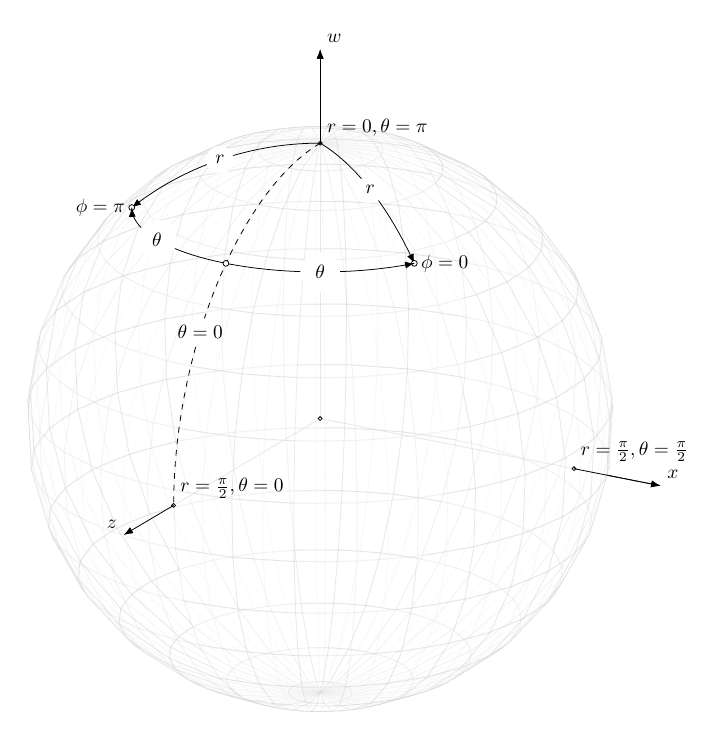
\begin{tikzpicture}[scale = 0.7,angle/.style={black,thick}]

\pgfplotsset{every axis/.append style={
view={120}{20},
%axis equal image,
    %clip=false,
    %xlabel=$x$, ylabel=$y$, zlabel=$z$,
    %axis lines=middle,
    colormap={whitered}{
        color(0cm)=(white);
        color(1cm)=(black!75!gray)
    }
    %y dir=reverse,
%    axis on top
            }}

\tikzmath{\p=360;\a=1/sqrt(0.05*0.05+0.1*0.1);\k=3;\f=1;\u1=0;\v1=0;\u2=0;\v2=0;\u3=0;\v3=0;\u4=0;\v4=0;};
\p, \a, \k,\u1,\v1,\u2,\v2,\u3,\v3,\u4,\v4,\f;
    %\pgfplotsset{ticks=none};
    \pgfplotsset{compat=1.12};
    \tikzset{>=latex} % for LaTeX arrow head
\begin{axis}
		[
		axis equal image,
		hide axis,clip=false,
		zmin=-\k,
		zmax=\k,
			xmin=-\k,
		xmax=\k,
			ymin=-\k,
		ymax=\k,
		]
				%relevant points
	\coordinate (O) at ({ 0},{0},{0});%origin
	\coordinate (X) at ({4* \k},{0},{0});%origin
	\coordinate (Y) at ({ 0},{4*\k},{0});%origin
	\coordinate (Z) at ({ 0},{0},{4*\k});%origin
	\draw[-Latex](O)--(X);
	\draw[-Latex](O)--(Y);
	\draw[-Latex](O)--(Z);

	\addplot3[surf,fill=white!50,domain=0:\p,domain y=0:\p,samples=30,faceted color=gray!50,mark=none, opacity=0.21,fill opacity = 0.45,thin]({\a*sin(x)*cos(y)},{\a*sin(x)*sin(y)},{\a*cos(x)});
	\node[{anchor=south east}] at (X){$z$};
	\node[{anchor=south west}] at (Y){$x$};
	\node[{anchor=south west}] at (Z){$w$};
			
 \coordinate (Q) at ({ 0},{0},{0.0});%origin
\draw[fill=white](Q) circle(1pt)node[{anchor=north west}]{$$};; 	
 \coordinate (Qx) at ({\a*sin(0)*cos(0)},{\a*sin(0)*sin(0)},{\a*cos(0)});%origin
 \node[{anchor=south west}] at (Qx){$r=0, \theta =\pi$};
\draw[fill=white](Qx) circle(1pt)node[{anchor=north west}]{$$};; 
 \coordinate (Qz) at ({\a*sin(90)*cos(0)},{\a*sin(90)*sin(0)},{\a*cos(90)});%origin
 \node[{anchor=south west}] at (Qz){$r=\frac{\pi}{2}, \theta =0$};
\draw[fill=white](Qz) circle(1pt)node[{anchor=north west}]{$$};; 
 \coordinate (Qw) at ({\a*sin(90)*cos(90)},{\a*sin(90)*sin(90)},{\a*cos(90)});%origin
 \node[{anchor=south west}] at (Qw){$r=\frac{\pi}{2}, \theta =\frac{\pi}{2}$};
\draw[fill=white](Qw) circle(1pt)node[{anchor=north west}]{$$};; 


\draw[dashed] plot[variable=\x,domain=0:\p/4,samples=30,thick]({\a*sin(\x)*cos(0)},{\a*sin(\x)*sin(0)},{\a*cos(\x)});

\draw [postaction=decorate,decoration={markings,
    mark=at position 1 with {\arrow{Latex}}}] plot[variable=\x,domain=0:\p/9,samples=30,thick]({\a*sin(\x)*cos(60)},{\a*sin(\x)*sin(60)},{\a*cos(\x)});
 \coordinate (Pp) at ({\a*sin(\p/9)*cos(60)},{\a*sin(\p/9)*sin(60)},{\a*cos(\p/9)});
\draw[fill=white](Pp) circle(1.5pt)node[{anchor=west}]{$\phi =0$};; 

\draw [postaction=decorate,decoration={markings,
    mark=at position 1 with {\arrow{Latex}}}] plot[variable=\x,domain=0:\p/9,samples=30,thick]({\a*sin(\x)*cos(60)},{-\a*sin(\x)*sin(60)},{\a*cos(\x)});

\coordinate (Pn) at ({\a*sin(\p/9)*cos(60)},{-\a*sin(\p/9)*sin(60)},{\a*cos(\p/9)});
\draw[fill=white](Pn) circle(1.5pt)node[{anchor=east}]{$\phi =\pi$};; 

\draw[postaction=decorate,decoration={markings,
    mark=at position 1 with {\arrow{Latex}}}] plot[variable=\x,domain=0:60,samples=30,thick]({\a*sin(\p/9)*cos(\x)},{\a*sin(\p/9)*sin(\x)},{\a*cos(\p/9)});
\draw [postaction=decorate,decoration={markings,
    mark=at position 1 with {\arrow{Latex}}}] plot[variable=\x,domain=0:60,samples=30,thick]({\a*sin(\p/9)*cos(\x)},{-\a*sin(\p/9)*sin(\x)},{\a*cos(\p/9)});
 \coordinate (Pm) at ({\a*sin(\p/9)*cos(0)},{-\a*sin(\p/9)*sin(0)},{\a*cos(\p/9)});
\draw[fill=white](Pm) circle(1.5pt)node[{anchor= west}]{$$};; 

 \coordinate (Ta) at ({\a*sin(\p/9)*cos(30)},{\a*sin(\p/9)*sin(30)},{\a*cos(\p/9)});%origin
\draw[white,fill=white](Ta) circle(10pt)node[black]{$\theta$};; 

\coordinate (Tb) at ({\a*sin(\p/9)*cos(30)},{-\a*sin(\p/9)*sin(30)},{\a*cos(\p/9)});%origin
\draw[white,fill=white](Tb) circle(10pt)node[black]{$\theta$};; 

 \coordinate (Tc)  at ({\a*sin(\p/9/2)*cos(60)},{\a*sin(\p/9/2)*sin(60)},{\a*cos(\p/9/2)});
\draw[white,fill=white](Tc) circle(7pt)node[black]{$r$};

\coordinate (Td)  at ({\a*sin(\p/9/2)*cos(60)},{-\a*sin(\p/9/2)*sin(60)},{\a*cos(\p/9/2)});
\draw[white,fill=white](Td) circle(7pt)node[black]{$r$};



\coordinate (Te)  at ({\a*sin(55)*cos(0)},{\a*sin(55)*sin(0)},{\a*cos(55)});
\draw[white,fill=white](Te) circle(7pt)node[black]{$\theta=0$};

 
	\draw[-Latex](Qx)--(Z);
	\draw[-Latex](Qz)--(X);
	\draw[-Latex](Qw)--(Y);
\end{axis}
\end{tikzpicture}
}\\
    \subfloat[]{
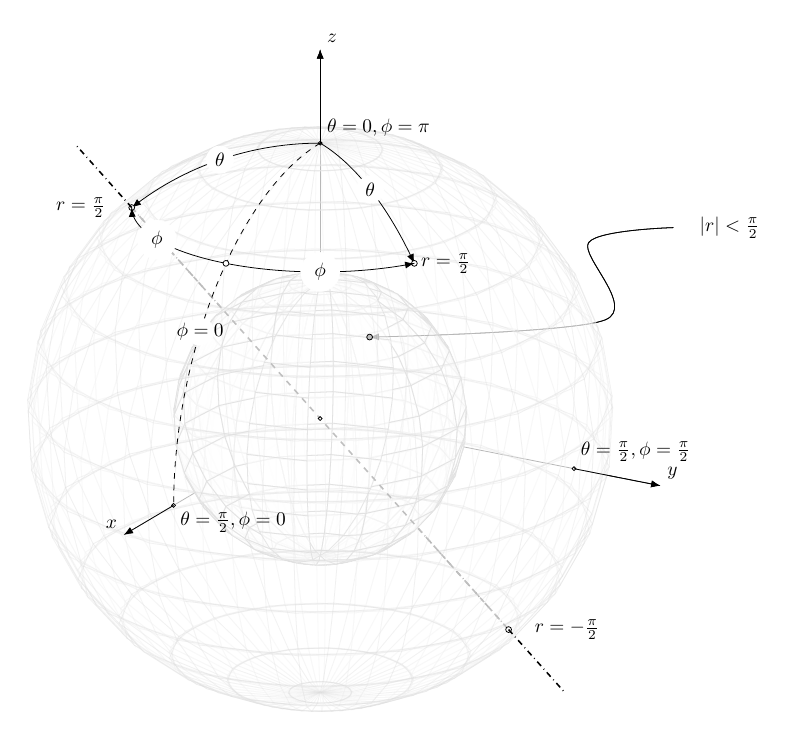
\begin{tikzpicture}[scale = 0.7,angle/.style={black,thick}]
\pgfplotsset{every axis/.append style={
view={120}{20},
axis equal image,
    %clip=false,
    %xlabel=$x$, ylabel=$y$, zlabel=$z$,
    %axis lines=middle,
    colormap={whitered}{
        color(0cm)=(white);
        color(1cm)=(black!75!gray)
    }
    %y dir=reverse,
%    axis on top
            }}
            
\tikzmath{\p=360;\a=1/sqrt(0.05*0.05+0.1*0.1);\k=3;\f=1;\u1=0;\v1=0;\u2=0;\v2=0;\u3=0;\v3=0;\u4=0;\v4=0;};
\p, \a, \k,\u1,\v1,\u2,\v2,\u3,\v3,\u4,\v4,\f;
    %\pgfplotsset{ticks=none};
    \pgfplotsset{compat=1.12};
    \tikzset{>=latex} % for LaTeX arrow head
\begin{axis}
		[axis equal image,
		hide axis,clip=false,
		zmin=-\k,
		zmax=\k,
			xmin=-\k,
		xmax=\k,
			ymin=-\k,
		ymax=\k,
		]
				%relevant points
	\coordinate (O) at ({ 0},{0},{0});%origin
	\coordinate (X) at ({4* \k},{0},{0});%origin
	\coordinate (Y) at ({ 0},{4*\k},{0});%origin
	\coordinate (Z) at ({ 0},{0},{4*\k});%origin
	\draw[-Latex](O)--(X);
	\draw[-Latex](O)--(Y);
	\draw[-Latex](O)--(Z);


\coordinate (Pn) at ({\a*sin(\p/9)*cos(60)},{-\a*sin(\p/9)*sin(60)},{\a*cos(\p/9)});
\coordinate (Pnn) at ({-\a*sin(\p/9)*cos(60)},{\a*sin(\p/9)*sin(60)},{-\a*cos(\p/9)});

\coordinate (Pnf) at ({1.3*\a*sin(\p/9)*cos(60)},{-1.3*\a*sin(\p/9)*sin(60)},{1.3*\a*cos(\p/9)});
\coordinate (Pnnf) at ({-1.3*\a*sin(\p/9)*cos(60)},{1.3*\a*sin(\p/9)*sin(60)},{-1.3*\a*cos(\p/9)});
\draw[dashdotted,thick](Pn)--(Pnn);
\coordinate (Pns) at ({1.05*\a*sin(\p/9)*cos(60)*sin(30)},{1.05*\a*sin(\p/9)*sin(60)*sin(30)},{1.05*\a*cos(\p/9)*sin(30)});
\coordinate (Pnsc) at ({\a*sin(\p/9)*cos(60)*1.5},{\a*sin(\p/9)*sin(60)*3},{\a*1.5*cos(\p/9)*1.});

	\draw[fill=black](Pns) circle(1.5pt)node[{anchor=west}]{$$};; 
	\draw[fill=white](Pnsc) circle(0pt)node[{anchor=west}]{$\quad |r|<\frac{\pi}{2}$};; 
	\draw []plot [smooth] coordinates {(Pnsc)  ({\a*sin(\p/9)*cos(60)*1.5},{0.8*\a*sin(\p/9)*sin(60)*3},{\a*cos(\p/9)*1.35})  ({\a*sin(\p/9)*cos(60)*1.5},{0.7*\a*sin(\p/9)*sin(60)*3.6},{\a*cos(\p/9)*1.}) (Pns)};

%draw surfaces
\addplot3[surf,fill=white!50,domain=0:\p,domain y=0:2*\p,samples=30,faceted color=gray!80,mark=none, opacity=0.8
	21,fill opacity = 0.65,thin]({\a*sin(1*30)*sin(x)*cos(y)},{\a*sin(1*30)*sin(x)*sin(y)},{\a*cos(x)*sin(1*30)});
\draw [-Latex]plot [smooth] coordinates {(Pnsc)  ({\a*sin(\p/9)*cos(60)*1.5},{0.8*\a*sin(\p/9)*sin(60)*3},{\a*cos(\p/9)*1.35})  ({\a*sin(\p/9)*cos(60)*1.5},{0.7*\a*sin(\p/9)*sin(60)*3.6},{\a*cos(\p/9)*1.}) (Pns)};

\addplot3[surf,fill=white!50,domain=0:\p,domain y=0:2*\p,samples=30,faceted color=gray!30,mark=none, opacity=0.21,fill opacity = 0.15,thin]({\a*sin(3*30)*sin(x)*cos(y)},{\a*sin(3*30)*sin(x)*sin(y)},{\a*cos(x)*sin(3*30)});

 \draw[dashed,thick, color = gray!50, opacity=1](Pn)--(Pnn);
	
	\node[{anchor=south east}] at (X){$x$};
	\node[{anchor=south west}] at (Y){$y$};
	\node[{anchor=south west}] at (Z){$z$};
			
 \coordinate (Q) at ({ 0},{0},{0.0});%origin
\draw[fill=white](Q) circle(1pt)node[{anchor=north west}]{$$};; 	
 \coordinate (Qx) at ({\a*sin(0)*cos(0)},{\a*sin(0)*sin(0)},{\a*cos(0)});%origin
 \node[{anchor=south west}] at (Qx){$\theta=0, \phi=\pi$};
\draw[fill=white](Qx) circle(1pt)node[{anchor=north west}]{$$};; 
 \coordinate (Qz) at ({\a*sin(90)*cos(0)},{\a*sin(90)*sin(0)},{\a*cos(90)});%origin
 \node[{anchor=north west}] at (Qz){$\theta=\frac{\pi}{2}, \phi =0$};
\draw[fill=white](Qz) circle(1pt)node[{anchor=north west}]{$$};; 
 \coordinate (Qw) at ({\a*sin(90)*cos(90)},{\a*sin(90)*sin(90)},{\a*cos(90)});%origin
 \node[{anchor=south west}] at (Qw){$\theta=\frac{\pi}{2}, \phi=\frac{\pi}{2}$};
\draw[fill=white](Qw) circle(1pt)node[{anchor=north west}]{$$};; 


\draw[dashed] plot[variable=\x,domain=0:\p/4,samples=30,thick]({\a*sin(\x)*cos(0)},{\a*sin(\x)*sin(0)},{\a*cos(\x)});

\draw [postaction=decorate,decoration={markings,
    mark=at position 1 with {\arrow{Latex}}}] plot[variable=\x,domain=0:\p/9,samples=30,thick]({\a*sin(\x)*cos(60)},{\a*sin(\x)*sin(60)},{\a*cos(\x)});
 \coordinate (Pp) at ({\a*sin(\p/9)*cos(60)},{\a*sin(\p/9)*sin(60)},{\a*cos(\p/9)});
\draw[fill=white](Pp) circle(1.5pt)node[{anchor=west}]{$r=\frac{\pi}{2}$};; 

\draw [postaction=decorate,decoration={markings,
    mark=at position 1 with {\arrow{Latex}}}] plot[variable=\x,domain=0:\p/9,samples=30,thick]({\a*sin(\x)*cos(60)},{-\a*sin(\x)*sin(60)},{\a*cos(\x)});

\draw[fill=white](Pn) circle(1.5pt)node[{anchor=east}]{$r=\frac{\pi}{2} \quad$};; 
\draw[fill=white](Pnn) circle(1.5pt)node[{anchor=west}]{$\quad r=-\frac{\pi}{2}$};; 



\draw[postaction=decorate,decoration={markings,
    mark=at position 1 with {\arrow{Latex}}}] plot[variable=\x,domain=0:60,samples=30,thick]({\a*sin(\p/9)*cos(\x)},{\a*sin(\p/9)*sin(\x)},{\a*cos(\p/9)});
\draw [postaction=decorate,decoration={markings,
    mark=at position 1 with {\arrow{Latex}}}] plot[variable=\x,domain=0:60,samples=30,thick]({\a*sin(\p/9)*cos(\x)},{-\a*sin(\p/9)*sin(\x)},{\a*cos(\p/9)});
 \coordinate (Pm) at ({\a*sin(\p/9)*cos(0)},{-\a*sin(\p/9)*sin(0)},{\a*cos(\p/9)});
\draw[fill=white](Pm) circle(1.5pt)node[{anchor= west}]{$$};; 

 \coordinate (Ta) at ({\a*sin(\p/9)*cos(30)},{\a*sin(\p/9)*sin(30)},{\a*cos(\p/9)});%origin
\draw[white,fill=white](Ta) circle(10pt)node[black]{$\phi$};; 

\coordinate (Tb) at ({\a*sin(\p/9)*cos(30)},{-\a*sin(\p/9)*sin(30)},{\a*cos(\p/9)});%origin
\draw[white,fill=white](Tb) circle(10pt)node[black]{$\phi$};; 

 \coordinate (Tc)  at ({\a*sin(\p/9/2)*cos(60)},{\a*sin(\p/9/2)*sin(60)},{\a*cos(\p/9/2)});
\draw[white,fill=white](Tc) circle(7pt)node[black]{$\theta$};

\coordinate (Td)  at ({\a*sin(\p/9/2)*cos(60)},{-\a*sin(\p/9/2)*sin(60)},{\a*cos(\p/9/2)});
\draw[white,fill=white](Td) circle(7pt)node[black]{$\theta$};



\coordinate (Te)  at ({\a*sin(55)*cos(0)},{\a*sin(55)*sin(0)},{\a*cos(55)});
\draw[white,fill=white](Te) circle(7pt)node[black]{$\phi=0$};

 \draw[dashdotted,thick](Pn)--(Pnf);

\draw[dashdotted,thick](Pnn)--(Pnnf);
	\draw[-Latex](Qx)--(Z);
	\draw[-Latex](Qz)--(X);
	\draw[-Latex](Qw)--(Y);
	\draw[fill=gray!50](Pns) circle(1.5pt)node[{anchor=west}]{$$};;

\end{axis}
\end{tikzpicture}}
\caption{Manifold with $ds^2=R^2\left[dr^2+\sin^2 r\left(d\theta^2+\sin^2\theta d\phi^2\right)\right]$ metric, embedded in a $4-$ Euclidean space}
\label{fig:fig_p265}
\end{figure}
$$\blacklozenge$$
\newpage
\setcounter{chapter}{7}
\chapter{Non-Riemannian spaces.}
\pagebreak[4]
%\begin{comment}
\section{p283 - Clarification}
\begin{tcolorbox}
$$\mathbf{8.101}\spatie \dv{T^{\rho}}{u} =\dv{T_r}{u}X^{\rho}_{r} + X^{\rho}_{rs}T^r \dv{x^s}{u}$$
\end{tcolorbox}
$T^r$ being a tensor, we have $ T^{\rho} = T^r X^{\rho}{r}$
, giving
\begin{align}
\dv{T^{\rho}}{u} &= X^{\rho}_{r}\dv{T_r}{u} + T^r dv{X^{\rho}_{r}}{u}\\
&= \dv{T_r}{u}X^{\rho}_{r} + T^r X^{\rho}_{rs}\dv{x^s}{u}
\end{align}
$$\blacklozenge$$
\newpage

\section{p284 - Clarification}
\begin{tcolorbox}
..., we immediately see that
$$\fdv{TS^r}{u} = \dv{T}{u} S^r + T \fdv{S^r}{u}$$
\end{tcolorbox}
We have 
\begin{align}
&\left\{\begin{array}{ll}
\fdv{S^r}{u} = \dv{S^r}{u} +\Gamma^r_{mn}S^m\dv{x^n}{u}& \ \\\\
\fdv{TS^r}{u} = \dv{TS^r}{u} +\Gamma^r_{mn}TS^m\dv{x^n}{u}& \ \\
\end{array}\right.\\
\Rightarrow \spatie &\left\{\begin{array}{ll}
T\fdv{S^r}{u} = T\dv{S^r}{u} +\Gamma^r_{mn}TS^m\dv{x^n}{u}&(a)\\\\
\fdv{TS^r}{u} = S^r\dv{T}{u} + T\dv{S^r}{u} +\Gamma^r_{mn}TS^m\dv{x^n}{u}&(b)\\
\end{array}\right.\\
(a)-(b)\Rightarrow\spatie & T \fdv{S^r}{u} - \fdv{TS^r}{u} =-  S^r\dv{T}{u} \\
\Rightarrow\spatie &\fdv{TS^r}{u} = T\fdv{S^r}{u}  +  S^r\dv{T}{u} 
\end{align}
$$\blacklozenge$$
\newpage

\section{p285 - Exercise}
\begin{tcolorbox}
Show that any tensor $T^{mn}$ may be written in the form
$$T^{mn}=X_{(p)}^{\ \ m}Y_{(p)}^{\ \ n}$$
and use this result to prove problem 11, Exercise III.
\end{tcolorbox}
The proof is the same as for $\mathbf{(8.107)}$ . Let's define $X^{(p) m}_{}=T^{mp}$ and $Y^{\ \ n}_{(p)}= \delta^n_p$. Then 
\begin{align}
S^{mn}&= X^{(p) m}_{} \delta^n_p\\
 &= X^{(n) m}_{}\\
 &=T^{mn}
\end{align}
$$\lozenge$$
Problem 11, Exercise III: $ T^{mn}_{\quad | mn}= T^{mn}_{\quad | nm}$\\
We can compose $T^{mn}$ in two equivalent ways:   $T^{mn} = X^{(p) m}_{}Y^{\ \ n}_{(p)}$ with $X^{(p) m}_{}=T^{mp}$and $Y^{\ \ n}_{(p)}= \delta^n_p$ and also $T^{mn} = X^{(p) n}_{}Y^{\ \ m}_{(p)}$ with $X^{(p) n}_{}=T^{pn}$and $Y^{\ \ m}_{(p)}= \delta^m_p$. \\
For the first we have obviously
\begin{align}
T^{mn}_{\quad | m}&= X^{(p) m}_{\quad \quad |m} \delta^n_p+ X^{(p) m}_{} \underbrace{\delta^n_{p|m}}_{=0}\\
&= X^{(p) m}_{\quad \quad | m} \delta^n_p\\
T^{mn}_{\quad \quad | mn}&= X^{(p) m}_{\quad \quad |mn} \delta^n_p+ X^{(p) m}_{\quad |m} \underbrace{\delta^n_{p|m}}_{=0}\\
&= X^{(p) m}_{\quad \quad |mn} \delta^n_p\\
&= X^{(n) m}_{\quad \quad |mn} 
= T^{mn}_{\quad | mn}
\end{align}
and for the second 
\begin{align}
T^{mn}_{\quad | n}&= X^{(p) n}_{\quad \quad |n} \delta^m_p+ X^{(p) n}_{} \underbrace{\delta^m_{p|n}}_{=0}\\
&= X^{(p) n}_{\quad \quad | n} \delta^m_p\\
T^{mn}_{\quad \quad | nm}&= X^{(p) n}_{\quad \quad |nm} \delta^m_p+ X^{(p) n}_{\quad |n} \underbrace{\delta^m_{p|m}}_{=0}\\
&= X^{(p) n}_{\quad \quad |nm} \delta^m_p\\
&= X^{(m) n}_{\quad \quad |nm} = T^{mn}_{\quad | nm}
\end{align}
$$\blacklozenge$$
\newpage


\section{p286 - Exercise}
\begin{tcolorbox}
Show that, if the parameter along the curve $x^r=x^r(u)$ is changed from $u$ to $v$, then the absolute derivative of a tensor field with respect to $v$ is $\dv{u}{v}$ times the abssolute derivative with rspect to $u$. Symbolically
$$\fdv{}{v}= \dv{u}{v}\fdv{}{u}$$
\end{tcolorbox}
Be $T^{rs\dots}_{mn\dots}$ an arbitrary tensor. Then,
\begin{align}
\fdv{}{v}T^{rs\dots}_{mn\dots} &= \dv{}{v}T^{rs\dots}_{mn\dots}+ \sum_{p} A^p_t \dv{x^t}{v} - \sum_{p} B_{pt} \dv{x^t}{v} 
\end{align}
with $A^p_t$ and $B_{pt}$ being the coefficients as functions of the Christoffels symbols and the tensor.
This expression can be expressed as 
\begin{align}
\fdv{}{v}T^{rs\dots}_{mn\dots} &= \dv{u}{v}\dv{}{u}T^{rs\dots}_{mn\dots}+ \sum_{p} A^p_t  \dv{u}{v}\dv{x^t}{u} - \sum_{p} B_{pt}  \dv{u}{v}\dv{x^t}{u} \\
&=\dv{u}{v}\fdv{}{u}T^{rs\dots}_{mn\dots}
\end{align}
$$\blacklozenge$$
\newpage

\section{p286 - Exercise}
\begin{tcolorbox}
Prove that $C^r_{mn}$ defined by 
$$\mathbf{8.114}\spatie C^r_{mn}=\Gamma^r_{mn}-\overline{\Gamma}^r_{mn}$$
is a tensor 
\end{tcolorbox}
Using $\mathbf{(8.112)}$ and $\mathbf{(8.113)}$ we get for a coordinate transformation
\begin{align}
C^{\rho}_{\mu \nu }&=\Gamma^{\rho}_{\mu \nu }-\overline{\Gamma}^{\rho}_{\mu \nu }\\
&= \Gamma^{r}_{mn}X^{\rho}_{r}X^{m}_{\mu}X^{n}_{\nu}+ X^{r}_{\mu \nu}X^{\rho}_{r}-\overline{\Gamma}^{r}_{mn}X^{\rho}_{r}X^{m}_{\mu}X^{n}_{\nu}- X^{r}_{\mu \nu}X^{\rho}_{r}\\
&= \left(\Gamma^{r}_{mn}- \overline{\Gamma}^{r}_{mn}\right) X^{\rho}_{r}X^{m}_{\mu}X^{n}_{\nu}
\end{align}
which is the transformation rule for a tensor 
$$\blacklozenge$$
\newpage



\section{p286 - Exercise}
\begin{tcolorbox}
Show that the right-hand side of $\mathbf{8.110}$ may also be obtained formally by the method of $\mathbf{(2.516)}$, i.e., by differentiating the invariant $T^{..r}_{mn}X^mY^nZ_r$, and using $\fdv{X^m}{u}=0$, $\fdv{Y^n}{u}=0$, $\fdv{Z_r}{u}=0$.
\end{tcolorbox}
Be $Q= T^{..r}_{mn}X^mY^nZ_r$ an invariant, then $\fdv{Q}{u}$ is also invariant and $\fdv{Q}{u} = \dv{Q}{u}$.
So,
\begin{align}
\dv{Q}{u}&= \dv{T^{..r}_{mn}}{u}X^mY^nZ_r+ T^{..r}_{mn}\left(\dv{X^m}{u}Y^nZ_r+X^m\dv{Y^n}{u}Z_r +X^mY^n\dv{Z_r}{u}\right)
\end{align}
where $X^m, \ Y^n, \ Z_r$ are transported parallely, hence  $$\fdv{X^m}{u} = 0, \ \fdv{Y^n}{u}=0 , \ \fdv{Z_r}{u}=0  $$
and 
$$\dv{X^m}{u} = -\Gamma^m_{pq}X^p\dv{x^q}{u}, \ \dv{Y^n}{u}=-\Gamma^n_{pq}Y^p\dv{x^q}{u} , \ \dv{Z_r}{u}=\Gamma^p_{rq}Z_p\dv{x^q}{u}  $$
giving
\begin{align}
\dv{Q}{u} &= \dv{T^{..r}_{mn}}{u}X^mY^nZ_r+ T^{..r}_{mn}\left(-\Gamma^m_{pq}X^p\dv{x^q}{u}Y^nZ_r  -\Gamma^n_{pq}Y^p\dv{x^q}{u}X^mZ_r+\Gamma^p_{rq}Z_p\dv{x^q}{u}X^mY^n\right)\\
&= \underbrace{\left(\dv{T^{..r}_{mn}}{u}-\Gamma^p_{mq}T^{..r}_{pn}\dv{x^q}{u} -\Gamma^p_{nq}T^{..r}_{mp}\dv{x^q}{u}+\Gamma^r_{pq}T^{..p}_{mn}\dv{x^q}{u}\right)}_{= \fdv{T^{..r}_{mn}}{u}}X^mY^nZ_r
\end{align}
Putting $   \fdv{T^{..r}_{mn}}{u} = \dv{T^{..r}_{mn}}{u}-\Gamma^p_{mq}T^{..r}_{pn}\dv{x^q}{u} -\Gamma^p_{nq}T^{..r}_{mp}\dv{x^q}{u}+\Gamma^r_{pq}T^{..p}_{mn}\dv{x^q}{u}$ is correct as from $$\fdv{Q}{u}= \fdv{T^{..r}_{mn}}{u}X^mY^nZ_r+ T^{..r}_{mn}\fdv{X_m}{u}Y^nZ_r+T^{..r}_{mn}\fdv{Y_{n}}{u}X^mZ_r+T^{..r}_{mn}\fdv{Z^{r}}{u}X^mY^n$$ and 
$$\fdv{X^m}{u} = 0, \ \fdv{Y^n}{u}=0 , \ \fdv{Z_r}{u}=0  $$
we get 
$$\fdv{Q}{u}= \fdv{T^{..r}_{mn}}{u}X^mY^nZ_r$$
as in $(3)$.  
$$\blacklozenge$$
\newpage




\section{p288 - Exercise}
\begin{tcolorbox}
Prove that $\delta^r_{s|n} = C^r_{sn}$ where $C^r_{sn}$ is defined by $\mathbf{(8.114)}$.
\end{tcolorbox}
\begin{align}
 \delta^r_{s|n} &=\underbrace{\delta^r_{s,n} }_{=0}+ \Gamma^r_{kn}\delta^k_s - \overline{\Gamma}^k_{sn}\delta^r_k\\
 &=\Gamma^r_{sn} - \overline{\Gamma}^r_{sn}\\
 &= C^r_{sn}
\end{align}
$$\blacklozenge$$
\\\\
\section{p288 - Exercise}
\begin{tcolorbox}
Prove that an invariant remains constant under parallel propagation.
\end{tcolorbox}
 $T$ invariant and transported parallely means $\fdv{T}{u}=\dv{T}{u}=0$ which implies $T=\text{constant}$
$$\blacklozenge$$
\newpage

\section{p289 - Exercise}
\begin{tcolorbox}
Show that by a suitable choice of the parameter $u$ along a path, the differential equation $\mathbf{(8.119)}$ simplifies to $\fdv{\lambda^r}{u}=0$.
\end{tcolorbox}
 The proof is similar to the clarification $2.17$ in part I and generalises the idea of null-geodesics.\\
 Suppose that we have indeed as in $\mathbf{(8.119)}$
 \begin{align}
 \fdv{\lambda^r}{u} = \mu(u)\lambda^r
 \end{align}
 Suppose now that we can find a suitable parameter $s$ for which
 \begin{align}
 \fdv{\lambda^r}{s} = 0
 \end{align}
 so 
 \begin{align}
 \fdv{\lambda^r}{s} = \dv[2]{x^r}{s}+\Gamma^r_{mn}\dv{x^m}{s}\dv{x^n}{s}=0
 \end{align}
 and suppose that there is an homeomorphism between $u$ and $s$, then we can write (see section $2.17$ for the details):
 \begin{align}
\dv[2]{x^r}{u}+\Gamma^r_{mn}\dv{x^m}{s}\dv{x^n}{s}=- \frac{\dv[2]{u}{s}}{\left(\dv{x^r}{s}\right)^2}\dv{x^r}{u}
 \end{align}
 and from$(1)$ we deduce 
 \begin{align}
 -\frac{\dv[2]{u}{s}}{\left(\dv{u}{s}\right)^2}= \mu(u)
 \end{align}
 This is a differential equation which gives (see section $2.17$ in part I for the details)
 \begin{align}
 \frac{\dv[2]{s}{u}}{\left(\dv{s}{u}\right)^2}= \mu(u)
 \end{align}
 giving a solution 
 \begin{align}
 s(u)&= \int_{u_0}^{u}\left(exp\left(\int_{v_0}^v\mu(v)dw\right)\right)dv
 \end{align}
 as a suitable parameter for which $$\fdv{\lambda^r}{s} = 0$$
$$\blacklozenge$$
\newpage



\section{p290 - Exercise}
\begin{tcolorbox}
Show that, in a space with ortho-invariant linear connection, the Kronecker delta is propagated parallely along curves satisfying $C_n\lambda^n = 0$.
\end{tcolorbox}
 \begin{align}
 \fdv{}{u}\delta^r_s &= \underbrace{\dv{}{u}\delta^r_s}_{=0}+\Gamma^r_{mn}\delta^m_s\dv{x^n}{u} - \overline{\Gamma}^m_{sn}\delta^r_m\dv{x^n}{u} \\
 &= \left(\Gamma^r_{mn}\delta^m_s - \overline{\Gamma}^m_{sn}\delta^r_m\right)\dv{x^n}{u} \\
 &=\underbrace{ \left(\Gamma^r_{sn} - \overline{\Gamma}^r_{sn}\right)}_{=C^r_{sn}}\dv{x^n}{u}\\
 &=C^r_{sn}\lambda^n 
 \end{align}
 Ortho-invariant linear connection means $C^r_{sn}=\delta^r_s C_n$, giving
  \begin{align}
 \fdv{}{u}\delta^r_s &= \delta^r_s C_n\lambda^n \\
 &=0
 \end{align}
 provided that $C_n\lambda^n = 0$.
$$\blacklozenge$$\\\\



\section{p292 - Exercise}
\begin{tcolorbox}
Show that in the case of a single connection,
$$\mathbf{8.127}  \spatie \fdv{}{u}\delta^r_s =0$$
\end{tcolorbox}
 From exercise page $290$, we have
 $$\fdv{}{u}\delta^r_s =  \left(\Gamma^r_{sn} - \overline{\Gamma}^r_{sn}\right)\dv{x^n}{u}$$ and for a single connection $\Gamma^r_{sn} = \overline{\Gamma}^r_{sn}$ from which we get
 $$\fdv{}{u}\delta^r_s =  0$$
$$\blacklozenge$$
\newpage



\section{p294 - Exercise}
\begin{tcolorbox}
Deduce immediately that from $F2$ that
$$T_{|mn}= T_{|nm}$$ where $T$ is an invariant.
\end{tcolorbox}
 From $F2$ we know that there exists a coordinate system for which the absolute derivative reduces to the ordinary derivative, hence $T_{,mn}= T_{,nm}$ . As $T$ is an invariant the identity holds for every coordinate system.
$$\blacklozenge$$\\

\section{p295 - Exercise}
\begin{tcolorbox}
\begin{align*}
\begin{array}{ll}
\mathbf{8.215}& R^s_{.rmn} = -R^s_{.rnm}\\
\mathbf{8.216}& R^s_{.rmn} + R^s_{.mnr}+ R^s_{.nrm}=0\\
\mathbf{8.217}& R^s_{.rmn|k} + R^s_{.rnk|m}+ R^s_{.rkm|n}=0
\end{array}
\end{align*}
Prove the above identities by using a coordinate system considered in $F2$.
\end{tcolorbox}
 At the origin of the coordinate syetm of the type considered in $F2$. We have 
 \begin{align}
 R^s_{.rmn}&= \Gamma^s_{rn,m}-\Gamma^s_{rm,n}\\
 \Rightarrow \spatie R^s_{.rnm}&= \Gamma^s_{rm,n}-\Gamma^s_{rn,m} = -R^s_{.rmn}
 \end{align}
 and 
 \begin{align}
 R^s_{.rmn} + R^s_{.mnr}+ R^s_{.nrm}&= \Gamma^s_{rn,m}-\Gamma^s_{rm,n} +\Gamma^s_{mr,n}-\Gamma^s_{mn,r} +\Gamma^s_{nm,r}-\Gamma^s_{nr,m} \\
 &=0
 \end{align}
 and 
 \begin{align}
 R^s_{.rmn|k} + R^s_{.rnk|m}+ R^s_{.rkm|n}&= \Gamma^s_{rn,mk}-\Gamma^s_{rm,nk} +\Gamma^s_{rk,nm}-\Gamma^s_{rn,km} +\Gamma^s_{rm,kn}-\Gamma^s_{rk,mn}\\
 &=0
 \end{align}
$$\blacklozenge$$
\newpage

\section{p295 - Exercise}
\begin{tcolorbox}
Verify that $F_{mn}$ is skew-symmetric and that $R_{mn}+F_{mn}$ is symmetric. Show also directly from $8.219$ that $F_{mn}$ vanishes in a Riemannian space?
\end{tcolorbox}
\begin{align}
F_{mn} &= \half\left( \Gamma^s_{ns,m}-\Gamma^s_{ms,n} \right)\\
F_{nm} &= \half\left( \Gamma^s_{ms,n}-\Gamma^s_{ns,m} \right)\\
&= -\half\left( \Gamma^s_{ns,m}-\Gamma^s_{ms,n} \right)
\end{align}
And, as for $m=n$, $F_{mn} = 0$, we can conclude that $F_{mn}$ is skew-symmetric.
$$\lozenge$$\\
\begin{align}
R_{mn} +F_{mn} &=  \Gamma^s_{ms,n}-\Gamma^s_{mn,s}+\half\left( \Gamma^s_{ns,m}-\Gamma^s_{ms,n} \right)+\Gamma^k_{ms}\Gamma^s_{kn}-\Gamma^k_{mn}\Gamma^s_{ks}\\
&=  \underbrace{\half \Gamma^s_{ms,n}-\Gamma^s_{mn,s}+\half \Gamma^s_{ns,m}}_{=\text{symmetric in } m,n} +\underbrace{\Gamma^k_{ms}\Gamma^s_{kn}}_{=\text{symmetric in } m,n}-\underbrace{\Gamma^k_{mn}\Gamma^s_{ks}}_{=\text{symmetric in } m,n}\\
\end{align}
Conclusion: $R_{mn} +F_{mn}$ is symmetric.
$$\lozenge$$\\
In Riemannian space we have $$F_{mn} = \half R^s_{.smn} = \half a^{sk}R_{ksmn}$$
As $a^{sk}= a^{ks}$ and $R_{ksmn}= - R_{skmn}$, this implies
$$F_{mn}=0$$ as wehave doubleterms of the form
\begin{align*}
a^{SK}R_{KSmn} + a^{KS}R_{SKmn} = a^{SK}R_{KSmn} - a^{SK}R_{KSmn} = 0
\end{align*}
$$\blacklozenge$$\\
\newpage

\section{p298 - Exercise}
\begin{tcolorbox}
Prove that $\mathbf{(8.301)}$ implies
$$\mathbf{8.310}\spatie a^{mn}_{\quad |r} - a^{mn}\phi_r=0$$
\end{tcolorbox}
We have 
\begin{align}
 a_{mn|r} + a_{mn}\phi_r=0
 \end{align}
 As $a^{mn}a_{mn}= N$ we have 
 \begin{align}
 &\left(a^{mn}a_{mn}\right)_{|r}=0\\
 \Rightarrow \spatie &a^{mn}a_{mn|r}=-a^{mn}_{\quad |r}a_{mn}\\
 (3) \text{ and } (1) \times a^{mn}:\spatie &-a^{mn}_{\quad |r}a_{mn}+ a^{mn}a_{mn}\phi_ra_{mn}=0\\
 \Rightarrow \spatie &a^{mn}_{\quad |r}-a^{mn}a_{mn}\phi_r-=0
 \end{align}
$$\blacklozenge$$\\

\section{p299 - Exercise}
\begin{tcolorbox}
Is $\delta^r_s$ a gauge invariant tensor?
\end{tcolorbox}
We have $\delta^n_r = a^{'}_{rk} a^{'kn} $ with (see $\mathbf{(8.311)}$) $a^{'}_{rk}= \lambda a^{'}_{rk} $.\\
From chapter II $\mathbf{(2.203)}$ we have 
\begin{align}
a^{'kn} &= \frac{\Delta^{'kn}}{a^{'}}
\end{align}
with
\begin{align}
\Delta^{'kn} &= \lambda^{N-1}\Delta^{kn}\\
a^{'}&= \lambda^N a\\
\Rightarrow\spatie a^{'kn} &= \frac{ 1}{\lambda} a^{kn}\\
\Rightarrow\spatie \delta^n_r &= \lambda a_{rk}\frac{ 1}{\lambda} a^{kn}\\
&= \delta^{kn} 
\end{align}
Hence, $ \delta^{kn} $ is gauge invariant.
$$\blacklozenge$$
\newpage
\section{p299 - Exercise}
\begin{tcolorbox}
Show that, under the gauge transformation $\mathbf{(8.311)}$, $a^{mn}$ and $a$ transforms as follows:
$$a^{'kn} = \frac{ 1}{\lambda} a^{kn},\quad a^{'}= \lambda^N a $$
\end{tcolorbox}
See previous exercise.
$$\blacklozenge$$\\

\section{p300 - Exercise}
\begin{tcolorbox}
The covariant curvature tensor is defined by $$R_{srmn} = a_{sp}R^s_{.rmn}$$.
How does it behave under gauge transformations?
\end{tcolorbox}
 $$R_{srmn} = a_{sp}R^s_{.rmn}$$
 $R^p_{.rmn} $ is gauge invariant, hence $R^{'p}_{.rmn} =R^p_{.rmn} $ and $a^{'}_{sp}= \lambda a^{}_{sp} $ giving
 
 \begin{align}
 R^{'}_{srmn} &=\lambda a^{}_{sp}R^p_{.rmn}\\
 &=\lambda R_{srmn}
 \end{align}
 Hence, $R_{srmn}$ is not gauge invariant.
$$\blacklozenge$$\\
\newpage


\section{p307 - Exercise 1}
\begin{tcolorbox}
In a space with a general linear connection,show that the expressions
$$\Gamma^r_{mn}- \Gamma^r_{nm}, \quad \overline{\Gamma}^r_{mb}- \overline{\Gamma}^r_{nm}$$ are tensors of the tpe indicated by the position of he suffixes.
\end{tcolorbox}
 We use $\mathbf{(8.112)}$ page $286$:
 \begin{align}
 \left\{\begin{array}{l}
 \Gamma^{\rho}_{\mu\nu} = \Gamma^{r}_{mn} X^{\rho}_r X^m_{\mu} X^n_{\nu} + X^r_{\mu \nu} X^{\rho}_r\\\\
 \overline{\Gamma}^{\rho}_{\mu\nu} = \overline{\Gamma}_{mn} X^{\rho}_r X^m_{\mu} X^n_{\nu} + X^r_{\mu \nu} X^{\rho}_r\\
 \end{array}\right.\\
 \Rightarrow\spatie \Gamma^{\rho}_{\mu\nu} -\Gamma^{\rho}_{\nu\mu}&=\Gamma^{r}_{mn} X^{\rho}_r X^m_{\mu} X^n_{\nu}-\Gamma^{r}_{nm} X^{\rho}_r X^n_{\mu} X^m_{\nu}\\
 &= \left(\Gamma^{r}_{mn}-\Gamma^{r}_{nm}\right)X^{\rho}_r X^m_{\mu} X^n_{\nu}
 \end{align}
 So, $\Gamma^{r}_{mn}-\Gamma^{r}_{nm}$ transforms as a tensor.
$$\blacklozenge$$\\
\newpage

\section{p308 - Exercise 2}
\begin{tcolorbox}
 If $T$ is an invariant in a space with a single linear connection, show that
 $$ T_{|mn} - T_{|nm} = -2 T_{|r} L^r_{mn}$$
 where 
 $$ L^r_{mn} = -L^r_{nm} = \half\left(\Gamma^r_{mn} - \Gamma^r_{nm}\right)$$
\end{tcolorbox}
For an invariant, yields
\begin{align}
&T_{|m} = T_{,m}\\
\Rightarrow\spatie T_{|mn}-T_{|nm} &= \underbrace{T_{,mn}-T_{,nm}}_{=0} -\overline{\Gamma}^k_{mn}T_{,k} + \overline{\Gamma}^k_{nm}T_{,k} \\
&= -\left(\Gamma^k_{mn}- \Gamma^k_{nm} \right) \underbrace{T_{,k}}_{= T_{|k}}\\
&= 2T_{|k}L^k_{mn}
\end{align}
with $ L^k_{mn} = \half\left(\Gamma^k_{mn}- \Gamma^k_{nm} \right) $

$$\blacklozenge$$\\
\newpage


\section{p308 - Exercise 3}
\begin{tcolorbox}
If $T_r$ is a covariant vector field in in a space with a single linear connection, show that
 $$ T_{r|mn} - T_{r|nm} = T_s R^s_{.rmn}-2 T_{|r} L^r_{mn}$$
 where $ L^r_{mn}$ is defined in Ex. $2$, and where 
 $$R^s_{.pm} = \Gamma^s_{rn,m} - \Gamma^s_{rm,n} + \Gamma^p_{rn}\Gamma^s_{pm}-\Gamma^p_{rm}\Gamma^s_{pn}$$
\end{tcolorbox}
Starting from $ T_{r|m} = T_{r,m} - \Gamma^p_{rm}T_p$ we get
\begin{align}
&\left\{\begin{array}{l}
T_{r|mn} = T_{r,mn} - \Gamma^p_{rm,n}T_p- \Gamma^p_{rm}T_{p,n} - \Gamma^q_{rn}T_{q,m} + \Gamma^q_{rn}\Gamma^p_{qm}T_{p} - \Gamma^q_{mn}T_{r,q} +  \Gamma^q_{mn}\Gamma^p_{rq}T_{p} \\\\
T_{r|nm} = T_{r,mn} - \Gamma^p_{rn,m}T_p- \Gamma^p_{rn}T_{p,m} - \Gamma^q_{rm}T_{q,n} + \Gamma^q_{rm}\Gamma^p_{qn}T_{p} - \Gamma^q_{nm}T_{r,q} +  \Gamma^q_{nm}\Gamma^p_{rq}T_{p} \\
\end{array}
\right.
\end{align}

\begin{align}
\Rightarrow\quad T_{r|mn} -T_{r|nm} &= \left\{\begin{array}{l}
 \left(\Gamma^p_{rn,m} - \Gamma^p_{rm,n} 
- \Gamma^q_{mn}\Gamma^p_{rq}+ \Gamma^q_{rn}\Gamma^p_{qm}- \Gamma^q_{rm}\Gamma^p_{qn}+  \Gamma^q_{mn}\Gamma^p_{rq}\right)T_p\\\
- \cancel{\Gamma^p_{rm}T_{p,n}} - \cancel{\Gamma^q_{rn}T_{q,m}}  - \Gamma^q_{mn}T_{r,q}   +  \cancel{\Gamma^p_{rn}T_{p,m}} + \cancel{\Gamma^q_{rm}T_{q,n}} + \Gamma^q_{mn}T_{r,q}  \\
\end{array}
\right.\\
&=  \left\{\begin{array}{l}
 \underbrace{\left(\Gamma^p_{rn,m} - \Gamma^p_{rm,n} 
+ \Gamma^q_{rn}\Gamma^p_{qm}- \Gamma^q_{rm}\Gamma^p_{qn}\right)}_{= R^p_{.rmn}}T_p\\\\
 +  \Gamma^q_{mn}\underbrace{\left(T_{r,q}- \Gamma^p_{rq}T_p\right)}_{= T_{r|q}} -  \Gamma^q_{nm}\underbrace{\left(T_{r,q}-\Gamma^p_{rq}T_p\right)}_{= T_{r|q}}
   \\
\end{array}
\right.\\
&= R^p_{.rmn}T_p-2T_{r|q}L^q_{mn}
\end{align}
$$\blacklozenge$$\\
\newpage



\section{p308 - Exercise 4}
\begin{tcolorbox}
In a space with a single linear connection, show that \textit{if} there exists a coordinate system for each point $O$ of space such that, at $O$ and for all curves through $O$, the absolute and ordinary derivatives of any tensor differ by a multiple of the tensor, \textit{then }the coefficients of linear connection satisfy a relationship of the form 
$$\Gamma^r_{mn}-\Gamma^r_{nm} = \delta^r_mA_n - \delta^r_n A_m$$
where $A_r$ is some covariant vector. (Such a single linear connection is said to be \textit{semi-symmetric}).
\end{tcolorbox}
Let's put $\Delta T_k = \dv{T_k}{u} - \fdv{T_k}{u}$, so
\begin{align}
\Delta T_k&= \Gamma^m_{kt}T_m\lambda^t\spatie (\lambda^t = \dv{x^t}{u}\text{ for any curve.})
\end{align}
Given is: $ \Delta T_k = \mu T_k$. So $(1)$ can be written as 
\begin{align}
\mu T_k&= \Gamma^m_{kt}T_m\lambda^t\\
\Leftrightarrow\spatie &= \left(\Gamma^m_{kt}\lambda^t\right)T_m\\
\Rightarrow\spatie \Gamma^m_{kt}\lambda^t &= \mu \delta^m_k
\end{align}
We can also write $(4)$ as $ \Gamma^m_{tk}\lambda^k = \mu \delta^m_t$
\begin{align}
\Rightarrow\spatie \Gamma^m_{kt}\lambda^t\lambda^k-\Gamma^m_{tk}\lambda^t\lambda^k &= \mu \left(\delta^m_k\lambda^k- \delta^m_t\lambda^t\right)\\
\Leftrightarrow\spatie \left(\Gamma^m_{kt}-\Gamma^m_{tk}\right)\lambda^t\lambda^k &= \mu \left(\lambda^m- \lambda^m\right)\\
&=0
\end{align}
As $(7)$ is true for every curve (every $\lambda^t$), we can conclude as a  trivial solution that $\Gamma^m_{kt}=\Gamma^m_{tk}$. But another solution makes $\left(\Gamma^m_{kt}-\Gamma^m_{tk}\right)\lambda^t\lambda^k  =0$, i.e. $ \Gamma^m_{kt}-\Gamma^m_{tk}= \delta^m_kA_t - \delta^m_tA_k $, indeed
\begin{align}
\left(\delta^m_kA_t - \delta^m_tA_k\right)\lambda^t\lambda^k &=  \lambda^mA_t\lambda^t-\lambda^mA_k\lambda^k\\
&=0
\end{align}
This  solution is less restrictive than the trivial solution. \\
As any tensor can be expressed as the outer product of $1-$forms, the proof is valid for any tensor of any rank.
$$\blacklozenge$$\\
\newpage



\section{p308 - Exercise 5}
\begin{tcolorbox}
Prove the converse of Exercise $4$.\\
Hint: Consider the coordinate transformation (in notation of $\mathbf{8.208}$):
$$x^{\rho} = \delta^{\rho}_r\left(x^r-x^r_0\right) + \half\left\{\half\delta^{\rho}_r\left(\Gamma^r_{mn} +\Gamma^r_{nm}\right)_0 - \frac{1}{N-1}\delta^{\rho}_n\left(\Gamma^p_{pm}-\Gamma^p_{mp}\right)_0 \right\}\left(x^m-x^m_0\right)\left(x^n-x^n_0\right)$$
\end{tcolorbox}
Be $T_r$ a random tensor at a point $O$ and a random curve $x^r=x^r(u)$.\\ Then 
\begin{align}\Delta T_r=  \dv{T_r}{u}-\fdv{T_r}{u}  =  \Gamma^m_{rn}T_m\lambda^n
\spatie (\lambda^n=\dv{x^n}{u})\end{align} 
let's used the proposed coordinate transformation and using that $\Gamma^p_{pm}-\Gamma^p_{mp} = \delta^p_pA_m - \delta^p_n A_p= \left(N-1\right)A_m$  at the point $O$, so the transformation reduces to
\begin{align}
x^{\rho} = \delta^{\rho}_r\left(x^r-x^r_0\right) + \half\left\{\half\delta^{\rho}_r\left(\Gamma^r_{mn} +\Gamma^r_{nm}\right)_0 - \delta^{\rho}_nA_{n(0)} \right\}\left(x^m-x^m_0\right)\left(x^n-x^n_0\right)
\end{align} 
Using $\mathbf{(8.211)}$ we get for a coordinate transformation:
\begin{align}
\Delta T_{\mu} &= \left( \Gamma^r_{mn}X_r^{\rho}X^m_{\mu}X^n_{\nu}- X_{mn}^{\rho}X^m_{\mu}X^n_{\nu} \right)X^s_{\rho}X^{\nu}_tT_s\lambda^t\\
&= \left( \Gamma^r_{mn}\delta_r^{s}X^m_{\mu}X^n_{\nu}\delta_t^{n}- X_{mn}^{\rho}X^s_{\rho}X^m_{\mu}\delta^n_{t} \right)T_s\lambda^t\\
&= \left( \Gamma^s_{mt}X^m_{\mu}- X_{mt}^{\rho}X^s_{\rho}X^m_{\mu} \right)T_s\lambda^t
\end{align}
and, using $(2)$  for the considered coordinate transformation:
\begin{align}
X^{\rho}_t &= \delta^{\rho}_r\delta^{r}_t + \half\left\{\half\delta^{\rho}_r\left(\Gamma^r_{mn} +\Gamma^r_{nm}\right)_0 - \delta^{\rho}_nA_{n(0)} \right\}\left(\delta^m_t x^n+\delta^n_t x^m-\delta^m_t x^n_0-\delta^n_t x^m_0\right)\\
&= \delta^{\rho}_t + \half\delta^{\rho}_r\left(\Gamma^r_{tn} +\Gamma^r_{nt}\right)_0\left(x^n - x^n_0 \right) - \half\left(\delta^{\rho}_n\left(x^n-x^n_0\right)A_{t(0)}+\delta^{\rho}_t\left(x^n-x^n_0\right)A_{n(0)} \right)
\end{align}
and 
\begin{align}
X^{\rho}_{tm} &= \half\left(\Gamma^r_{tm} +\Gamma^r_{mt}\right)_0\delta^{\rho}_r- \half \delta^{\rho}_m A_{t(0)}- \half \delta^{\rho}_t A_{m(0)}
\end{align}
giving for $(5)$:
\begin{align}
\Delta T_{\mu} &= \left[ \Gamma^s_{mt}X^m_{\mu}- \left(\half\left(\Gamma^r_{tm} +\Gamma^r_{mt}\right)_0\delta^{\rho}_r- \half \delta^{\rho}_m A_{t(0)}- \half \delta^{\rho}_t A_{m(0)}\right)X^s_{\rho}X^m_{\mu} \right]T_s\lambda^t\\
 &= \left[ \Gamma^s_{mt}X^m_{\mu}- \half\left(\Gamma^r_{tm} -\Gamma^r_{mt}\right)_0\delta^{s}_rX^m_{\mu}+ \half \delta^{s}_m A_{t(0)}X^m_{\mu}+ \half \delta^{s}_t A_{m(0)}X^m_{\mu}\right]T_s\lambda^t\\
 &= \left[ \half\underbrace{\left(\Gamma^s_{mt}-\Gamma^s_{tm} -\right)_0}_{=\delta^s_mA_{t(0)} - \delta^s_t A_{m(0)}}X^m_{\mu}+ \half \delta^{s}_m A_{t(0)}X^m_{\mu}+ \half \delta^{s}_t A_{m(0)}X^m_{\mu}\right]T_s\lambda^t\\
 &= \left[ \half\delta^s_mA_{t(0)} X^m_{\mu}- \half\delta^s_t A_{m(0)}X^m_{\mu}+ \half \delta^{s}_m A_{t(0)}X^m_{\mu}+ \half \delta^{s}_t A_{m(0)}X^m_{\mu}\right]T_s\lambda^t\\
 &=  \delta^s_mA_{t(0)} X^m_{\mu}T_s\lambda^t\\
 &= \underbrace{\left(A_{t(0)} \lambda^t\right)}_{\text{invariant}}\underbrace{T_sX^s_{\mu}}_{= T_{\mu}}
\end{align}
and we get $$\Delta T_{\mu}= kT_{\mu}$$.
$$\blacklozenge$$\\
\newpage



\section{p308 - Exercise 6}
\begin{tcolorbox}
Show that $$T_{r|s} - T_{s|r}= T_{r,s}-T_{s,r}$$
$T_r$ being a covariant vector, if the connection is symmetric but not, if the connection is unsymmetric.
\end{tcolorbox}
$T_{r|s} = T_{r,s}-\Gamma^m_{rs}T_m$ and $T_{s|r} = T_{s,r}-\Gamma^m_{sr}T_m$
So if the linear connection is symmetric
\begin{align}
T_{r|s} - T_{s|r}&= T_{r,s}-\Gamma^m_{rs}T_m-T_{s,r}+\Gamma^m_{sr}T_m
&= T_{r,s}-T_{s,r}
\end{align}\\
This is obviously not true for a non-symmetric linear connection.
$$\blacklozenge$$\\
\newpage

\section{p308 - Exercise 7}
\begin{tcolorbox}
Show that, in the generalized Stokes' theorem $\mathbf{(7.505)}$, the partial derivatives in the integrand on the left-hand side can be replaced by the covariant derivative if the space has a symmetric connection.
\end{tcolorbox}
\begin{align}
\mathbf{(7.505):}\spatie \int_{R_{(M)}} T_{k_1\dots k_{M-1},k_M}d\tau_{(M1)}^{k_1\dots k_{M-1}}&= \int_{R_{(M-1)}} T_{k_1\dots k_{M-1},k_M}d\tau_{(M-1)}^{k_1\dots k_{M-1}}
\end{align}
and we have 
\begin{align}
\int_{R_{(M)}} T_{k_1\dots k_{M-1}|k_M}d\tau_{(M1)}^{k_1\dots k_{M-1}}&= \left\{\begin{array}{l}
\int_{R_{(M)}} T_{k_1\dots k_{M-1},k_M}d\tau_{(M1)}^{k_1\dots k_{M-1}}\\\\
-\int_{R_{(M)}} \Gamma^{k_{\rho}}_{k_1 k_M}T_{k_{\rho}\dots k_{M-1},k_M}d\tau_{(M1)}^{k_1\dots k_{M-1}}\\\\
-\int_{R_{(M)}} \Gamma^{k_{\rho}}_{k_2 k_M}T_{k_1 k_{\rho}\dots k_{M-1},k_M}d\tau_{(M1)}^{k_1\dots k_{M-1}}\\\\
\spatie \spatie \vdots\\\\
-\int_{R_{(M)}} \Gamma^{k_{\rho}}_{k_{M-1} k_M}T_{k_1\dots k_{\rho},k_M}d\tau_{(M1)}^{k_1\dots k_{M-1}}
\end{array}\right.
\end{align}
We note that in the terms with the negative sign that $d\tau_{(M1)}^{k_1\dots k_{M-1}}$ is skew-symmetric. So, under the integral we will have two cancelling terms of sums of the form 

$$ \Gamma^{u}_{k_p k_M}T_{\dots u \dots ,k_M}d\tau_{(M1)}^{k_1\dots (k_p)\dots (k_{M})}+\Gamma^{u}_{k_M k_p }T_{\dots u \dots ,k_M}d\tau_{(M1)}^{k_1\dots (k_{M})\dots (k_p)}$$
As $\Gamma^{u}_{k_p k_M}$ is symmetric and  $d\tau_{(M1)}^{k_1\dots (k_{M})\dots (k_p)}$ skew-symmetric, the two sums cancel each other and we get the straight form of the Stokes theorem.
$$\blacklozenge$$\\
\newpage


\section{p309 - Exercise 8}
\begin{tcolorbox}
In a Weyl space, the rate of change of the squared magnitude $X^2$of a vector $X^r$ under parallel propagation of $X^r$ along some curve $x^r=x^r(u)$ is given  by
$$ \frac{\Delta}{\Delta u} X^2 = \dv{}{u}\left(\epsilon a_{mn}X^mX^n\right) = \epsilon \dv{a_{mn}}{u}X^mX^n +2\epsilon a_{mn} X^m\dv{X^n}{u}$$
where $\dv{a_{mn}}{u}$ is the ordinary derivative along the curve of $a_{mn}$ (which is defined throughout the space), whereas $\dv{X^r}{u}$ is obtained by parallel propagation, i.e.,
$$\dv{X^n}{u} = -\Gamma^n_{sp}X^s\dv{x^p}{u}$$
Show that 
$$\frac{\Delta}{\Delta u} X^2 = -X^2\phi_r\dv{x^r}{u}$$
Hence, prove that the change in $X^2$ under parallel propagation of $X^r$ around an infinitesimal circuit, bounding a $2-$element of extension $d\tau_{(2)}^{mn}$, is given by
$$\Delta X^2= \frac{2}{N}X^2F_{mn}d\tau_{(2)}^{mn}$$
(Hint: Use Stokes' theorem).
\end{tcolorbox}
We have in a space with symmetric linear connections
\begin{align}
\fdv{a_{mn}}{u} &= \dv{a_{mn}}{u} - \Gamma^k_{mt} a_{kn}\lambda^t - \Gamma^k_{nt} a_{mk}\lambda^t
\end{align}
and 
\begin{align}
\fdv{a_{mn}}{u} &= a_{mn|k}\lambda^k
\end{align}
and (Weyl space)
\begin{align}
a_{mn|k}+ a_{mn}\phi_k=0
\end{align}
Combining $(1),\ (2),\ (3)$ we get
\begin{align*}
-a_{mn}\phi_k\lambda_k &= \dv{a_{mn}}{u} - \Gamma^k_{mt} a_{kn}\lambda^t - \Gamma^k_{nt} a_{mk}\lambda^t\\
\Rightarrow\spatie \dv{a_{mn}}{u} &= \left(-a_{mn}\phi_t + \Gamma^k_{mt} a_{kn} + \Gamma^k_{nt} a_{mk}\right)\lambda^t
\end{align*}
From this expression and $ \dv{X^n}{u} = -\Gamma^n_{sp}X^s\lambda^p$ we get
\begin{align*}
\frac{\Delta}{\Delta u} X^2 &=\epsilon\left(-a_{mn}\phi_t + \Gamma^k_{mt} a_{kn} + \Gamma^k_{nt} a_{mk}\right)\lambda^tX^mX^n -2\epsilon a_{mn} X^m\Gamma^n_{sp}X^s\lambda^p\\
&=-\epsilon a_{mn}\phi_t\lambda^tX^mX^n  + \cancel{\epsilon\Gamma^k_{mt} a_{kn}\lambda^tX^mX^n }+ \cancel{\epsilon \Gamma^k_{nt} a_{mk}X^mX^n\lambda^t } -\cancel{\epsilon a_{mn}\Gamma^n_{sp X^m}X^s\lambda^p}-\cancel{\epsilon a_{mn} \Gamma^n_{sp}X^mX^s\lambda^p}\\
&=-\epsilon a_{mn}X^mX^n \phi_t \lambda^t
\end{align*}
but $X^2= \epsilon a_{mn} X^mX^n$, so
$$\frac{\Delta}{\Delta u} X^2 = -X^2\phi_t  \lambda^t$$


$$\lozenge$$


Applying Stokes' theorem to $\frac{\Delta}{\Delta u} X^2$
\begin{align}
 \int_{R_{(1)}} \Delta X^2 =\int_{R_{(1)}} \frac{\Delta}{\Delta u} X^2 du=-\int_{R_{(1)}}X^2\phi_r  dx^{r}= - \int_{R_{(2)}} \left( X^2\phi_r\right)_{,s}d\tau_{(2)}^{rs}
\end{align}
Taking the limit to an infinitesimal $2-$space $R_{(1)}\rightarrow dx^{r}$ and $R_{(2)}\rightarrow d\tau_{(2)}^{rs}$ we can write
\begin{align}
\Delta X^2  &= - \left( X^2\phi_r\right)_{,s}d\tau_{(2)}^{rs}\\
&= - \left[\left( X^2\right)_{,s}\phi_r + X^2\phi_{r,s} \right]d\tau_{(2)}^{rs}\\
&= - \left[ \left( X^2\right)_{,s}\phi_r + \half X^2\phi_{r,s} \right]d\tau_{(2)}^{rs}\\
&= \half X^2\left(\phi_{s,r}- \phi_{r,s} \right)d\tau_{(2)}^{rs} -  \left( X^2\right)_{,s}\phi_rd\tau_{(2)}^{rs} 
\end{align}
(the last step used the skew-symmetricity of $d\tau_{(2)}^{rs}$).\\

We have $F_{rs} = \frac{N}{4}\left(\phi_{s,r}- \phi_{r,s} \right)$, giving
\begin{align}
\Delta X^2  &= \frac{2}{N}F_{rs}  X^2 d\tau_{(2)}^{rs} -  \left( X^2\right)_{,s}\phi_rd\tau_{(2)}^{rs} 
\end{align}
Let's put $K\equiv \left( X^2\right)_{,s}\phi_rd\tau_{(2)}^{rs} $ and as we have $X^2= a_{mn}X^mX^n$
\begin{align}
K&=\left(a_{mn}X^mX^n\right)_{,s}\phi_r d\tau_{(2)}^{rs}\\
&=a_{mn,s}X^mX^n \phi_r d\tau_{(2)}^{rs}+2a_{mn}X^mX^n_{,s}\phi_r d\tau_{(2)}^{rs}
\end{align}
From $\mathbf{(8.304)}$ we have
\begin{align}
a_{mn,s} -\Gamma^k_{ms}a_{kn}- \Gamma^k_{nk}a_{km}+a_{mn}\phi_s=0
\end{align} 
and $(11)$ can be written as 

\begin{align}
K&= \Gamma^k_{ms}a_{kn}X^mX^n \phi_r d\tau_{(2)}^{rs}+ \Gamma^k_{ns}a_{km}X^mX^n \phi_r d\tau_{(2)}^{rs}-a_{mn}\phi_s X^mX^n \phi_r d\tau_{(2)}^{rs}+2a_{mn}X^mX^n_{,s}\phi_r d\tau_{(2)}^{rs}\\
&= 2\Gamma^k_{ms}a_{kn}X^mX^n \phi_r d\tau_{(2)}^{rs}-\underbrace{a_{mn}\phi_s X^mX^n \phi_r d\tau_{(2)}^{rs}}_{=0}+2a_{mn}X^mX^n_{,s}\phi_r d\tau_{(2)}^{rs}\\
&= 2\underbrace{\left(\Gamma^m_{ks}X^k +X^m_{,s}\right)}_{X^m_{\ |s}}a_{mn}X^n\phi_r d\tau_{(2)}^{rs}
\end{align}
We can put $X^m_{\ |s}=0$ as we can  span the infinitesimal $2-$space by a bundle of curves along which we parallely transport $X^m$.
So, $K=0$ and $(9)$ becomes
$$\Delta X^2  = \frac{2}{N}F_{rs}  X^2 d\tau_{(2)}^{rs}$$

$$\blacklozenge$$\\
\newpage


\section{p309 - Exercise 9}
\begin{tcolorbox}
Verify that the projective curvature tensor $\mathbf{8.338}$ is invariant under all projective transformations.
\end{tcolorbox}
We have
\begin{align}
\left\{\begin{array}{ll}
\mathbf{(8.338)}&W^s_{.rmn}=R^s_{.rmn}-\frac{2}{N+1}\delta_r^s F_{mn}+\frac{1}{N-1}\left(\delta^s_m R_{rn}-\delta^s_n R_{rm}\right)-\frac{2}{N^2-1}\left(\delta^s_n F_{rm}-\delta^s_mF_{rn}\right)\\\\
\mathbf{(8.214)}&R^{s}_{.rmn} = \Gamma^{s}_{rn,m} - \Gamma^{s}_{rm,n}+\Gamma^{p}_{rn}\Gamma^{s}_{pm}-\Gamma^{p}_{rm}\Gamma^{s}_{pn}\\\\
\mathbf{(8.219)}&F_{mn} = \half\left(\Gamma^{s}_{ns,m} - \Gamma^{s}_{ms,n}\right)\\
\end{array}
\right.
\end{align}
using a projective transformation of the form $\mathbf{(8.337)}$, we get 

\begin{align}
\left\{\begin{matrix}
\Gamma^{'s}_{rn,m} = \Gamma^{s}_{rn,m} +\delta^s_n\psi_{r,m} +\delta^s_r\psi_{n,m}\\\\
\Gamma^{'s}_{rm,n} = \Gamma^{s}_{rm,n} +\delta^s_m\psi_{r,n} +\delta^s_r\psi_{m,n}\\\\
\Gamma^{'s}_{ns,m} = \Gamma^{s}_{ns,m} +\delta^s_s\psi_{n,m} +\delta^s_n\psi_{s,m}= \Gamma^{s}_{ns,m} +\left(N+1\right)\psi_{n,m} \\\\
\Gamma^{'s}_{ms,n} = \Gamma^{s}_{ms,n} +\delta^s_s\psi_{m,n} +\delta^s_m\psi_{s,n}= \Gamma^{s}_{ms,n} +\left(N+1\right)\psi_{m,n} \\\\
\Gamma^{'s}_{rs,m} = \Gamma^{s}_{rs,m} +\delta^s_s\psi_{r,m} +\delta^s_r\psi_{s,m}= \Gamma^{s}_{rs,m} +\left(N+1\right)\psi_{r,m} \\\\
\Gamma^{'s}_{rs,n} = \Gamma^{s}_{rs,n} +\delta^s_s\psi_{r,n} +\delta^s_r\psi_{s,n}= \Gamma^{s}_{rs,n} +\left(N+1\right)\psi_{r,n} \\\\
\Gamma^{'p}_{rn} = \Gamma^{p}_{rn} +\delta^p_n\psi_r +\delta^p_r\psi_n\\\\
\Gamma^{'s}_{pm} = \Gamma^{s}_{pm} +\delta^s_m\psi_p +\delta^s_p\psi_m\\\\
\Gamma^{'p}_{rm} = \Gamma^{p}_{rm} +\delta^p_m\psi_r +\delta^p_r\psi_m\\\\
\Gamma^{'s}_{pn} = \Gamma^{s}_{pn} +\delta^s_n\psi_p +\delta^s_p\psi_n\\\\
\end{matrix}\right.\\
\end{align}
giving
\begin{align}
R^{'s}_{.rmn} &= \Gamma^{'s}_{rn,m} - \Gamma^{'s}_{rm,n}+\Gamma^{'p}_{rn}\Gamma^{'s}_{pm}-\Gamma^{'p}_{rm}\Gamma^{'s}_{pn}\\
&=\left\{\begin{matrix}
R^{s}_{.rmn}\\\\
+\delta^s_n\psi_{r,m} +\delta^s_r\psi_{n,m}-\delta^s_m\psi_{r,n} -\delta^s_r\psi_{m,n}\\\\
+\left(\delta^p_n\psi_r +\delta^p_r\psi_n\right) \Gamma^{s}_{pm}\\\\
+\Gamma^{p}_{rn}\left(\delta^s_m\psi_p +\delta^s_p\psi_m\right)\\\\
-\left(\delta^p_m\psi_r +\delta^p_r\psi_m\right)\Gamma^{s}_{pn}\\\\
-\Gamma^{p}_{rm}\left(\delta^s_n\psi_p +\delta^s_p\psi_n\right)\\\\
+\left(\delta^p_n\psi_r +\delta^p_r\psi_n\right) \left(\delta^s_m\psi_p +\delta^s_p\psi_m\right)\\\\
-\left(\delta^p_m\psi_r +\delta^p_r\psi_m\right)\left(\delta^s_n\psi_p +\delta^s_p\psi_n\right)\\
\end{matrix}\right.\\
&=\left\{\begin{matrix}
R^{s}_{.rmn}\\\\
+\delta^s_n\psi_{r,m} +\delta^s_r\psi_{n,m}-\delta^s_m\psi_{r,n} -\delta^s_r\psi_{m,n}\\\\
+\delta^p_n\psi_r\Gamma^{s}_{pm} +\delta^p_r\psi_n \Gamma^{s}_{pm}\\\\
+\delta^s_m\psi_p\Gamma^{p}_{rn} +\delta^s_p\psi_m\Gamma^{p}_{rn}\\\\
-\delta^p_m\psi_r\Gamma^{s}_{pn} -\delta^p_r\psi_m\Gamma^{s}_{pn}\\\\
-\Gamma^{p}_{rm}\delta^s_n\psi_p -\Gamma^{p}_{rm}\delta^s_p\psi_n\\\\
+\delta^p_n\psi_r\delta^s_m\psi_p +\delta^p_n\psi_r\delta^s_p\psi_m +\delta^p_r\psi_n\delta^s_m\psi_p  +\delta^p_r\psi_n \delta^s_p\psi_m\\\\
-\delta^p_m\psi_r \delta^s_n\psi_p -\delta^p_m\psi_r \delta^s_p\psi_n-\delta^p_r\psi_m\delta^s_n\psi_p -\delta^p_r\psi_m\delta^s_p\psi_n\\
\end{matrix}\right.
\end{align}
\begin{align}
&=\left\{\begin{matrix}
R^{s}_{.rmn}\\\\
+\delta^s_n\psi_{r,m} +\delta^s_r\psi_{n,m}-\delta^s_m\psi_{r,n} -\delta^s_r\psi_{m,n}\\\\
+\cancel{\psi_r\Gamma^{s}_{nm}} +\cancel{\psi_n \Gamma^{s}_{rm}}\\\\
+\delta^s_m\psi_p\Gamma^{p}_{rn} +\cancel{\psi_m\Gamma^{s}_{rn}}\\\\
-\cancel{\psi_r\Gamma^{s}_{mn}} -\cancel{\psi_m\Gamma^{s}_{rn}}\\\\
-\Gamma^{p}_{rm}\delta^s_n\psi_p -\cancel{\Gamma^{s}_{rm}\psi_n}\\\\
+\cancel{\delta^s_m\psi_n\psi_r} +\cancel{\delta^s_n\psi_m\psi_r }+\delta^s_m\psi_r\psi_n  +\cancel{\delta^s_r\psi_m\psi_n} \\\\
-\cancel{\delta^s_n\psi_r \psi_m }-\cancel{\delta^s_m\psi_r \psi_n}-\delta^s_n\psi_r\psi_m -\cancel{\delta^s_r\psi_m\psi_n}\\
\end{matrix}\right.\\
&=\left\{\begin{matrix}
R^{s}_{.rmn}\\\\
+\delta^s_n\psi_{r,m} +\delta^s_r\psi_{n,m}-\delta^s_m\psi_{r,n} -\delta^s_r\psi_{m,n}\\\\
+\delta^s_m\psi_p\Gamma^{p}_{rn} 
-\delta^s_n\psi_p \Gamma^{p}_{rm}
+\delta^s_m\psi_r\psi_n  -\delta^s_n\psi_r\psi_m 
\end{matrix}\right.
\end{align}
and
\begin{align}
F^{'}_{mn} &= \half\left(\Gamma^{s}_{ns,m} - \Gamma^{s}_{ms,n}\right)\\
&=F^{}_{mn} + \half\left(N+1\right)\left(\psi_{n,m} -\psi_{m,n}\right)
\end{align}
and
\begin{align}
R^{'}_{rm} &= \left\{\begin{matrix}
R^{}_{.rm}\\\\
+\delta^s_s\psi_{r,m} +\delta^s_r\psi_{s,m}-\delta^s_m\psi_{r,s} -\delta^s_r\psi_{m,s}\\\\
+\delta^s_m\psi_p\Gamma^{p}_{rs} 
-\delta^s_s\psi_p \Gamma^{p}_{rm}
+\delta^s_m\psi_r\psi_s  -\delta^s_s\psi_r\psi_m 
\end{matrix}\right.\\
&=\left\{\begin{matrix}
R^{}_{.rm}\\\\
+N\psi_{r,m} +\cancel{\psi_{r,m}}-\cancel{\psi_{r,m}} -\psi_{m,r}\\\\
+\psi_p\Gamma^{p}_{rm} 
-N\psi_p \Gamma^{p}_{rm}
+\psi_r\psi_m  -N\psi_r\psi_m 
\end{matrix}\right.\\
&=R^{}_{.rm}
+N\psi_{r,m} -\psi_{m,r} -\left(N-1\right) \Gamma^{p}_{rm}\psi_p
-\left(N-1\right)\psi_r\psi_m  
\end{align}
and
\begin{align}
R^{'}_{rn} &=R^{}_{.rn}
+N\psi_{r,n} -\psi_{n,r} -\left(N-1\right) \Gamma^{p}_{rn}\psi_p
-\left(N-1\right)\psi_r\psi_n  
\end{align}


When using a projective transformation of the form $\mathbf{(8.337)}$ (where $\psi_k$ is a random vector) and we calculate $\Delta W = W^{'s}_{.rmn}-W^s_{.rmn}$ , only terms containing $\psi_k$ will remain and we get
\begin{align}
\Delta W&= \left\{ \begin{matrix}
\delta^s_n\psi_{r,m} +\delta^s_r\psi_{n,m}-\delta^s_m\psi_{r,n} -\delta^s_r\psi_{m,n}\\\\
+\delta^s_m\psi_p\Gamma^{p}_{rn} 
-\delta^s_n\psi_p \Gamma^{p}_{rm}
+\delta^s_m\psi_r\psi_n  -\delta^s_n\psi_r\psi_m \\\\
-\frac{2}{N+1}\delta^s_r  \half\left(N+1\right)\left(\psi_{n,m} -\psi_{m,n}\right)\\\\
+\frac{1}{N-1}\left(\delta^s_m \left(N\psi_{r,n} -\psi_{n,r} -\left(N-1\right) \Gamma^{p}_{rn}\psi_p
-\left(N-1\right)\psi_r\psi_n \right)\right)\\\\-\frac{1}{N-1}\left(\delta^s_n \left(N\psi_{r,m} -\psi_{m,r} -\left(N-1\right) \Gamma^{p}_{rm}\psi_p
-\left(N-1\right)\psi_r\psi_m\right)\right)\\\\
-\frac{2}{N^2-1}\left(\delta^s_n  \half\left(N+1\right)\left(\psi_{r,m} -\psi_{m,r}\right)-\delta^s_m \half\left(N+1\right)\left(\psi_{n,r} -\psi_{r,n}\right)\right)
\end{matrix}\right.\\
&= \left\{ \begin{matrix}
\delta^s_n\psi_{r,m} +\cancel{\delta^s_r\psi_{n,m}}-\delta^s_m\psi_{r,n} -\cancel{\delta^s_r\psi_{m,n}}\\\\
+\delta^s_m\psi_p\Gamma^{p}_{rn} -\delta^s_n\psi_p \Gamma^{p}_{rm}
+\delta^s_m\psi_r\psi_n  -\delta^s_n\psi_r\psi_m \\\\
-\cancel{\delta^s_r\psi_{n,m}}+\cancel{\delta^s_r\psi_{m,n}}\\\\
+\frac{N}{N-1}\delta^s_m \psi_{r,n} -\frac{1}{N-1}\delta^s_m \psi_{n,r} - \delta^s_m \Gamma^{p}_{rn}\psi_p
-\delta^s_m \psi_r\psi_n \\\\
-\frac{1}{N-1}\delta^s_nN\psi_{r,m} +\frac{1}{N-1}\delta^s_n\psi_{m,r} + \delta^s_n\Gamma^{p}_{rm}\psi_p
+\delta^s_n\psi_r\psi_m\\\\
-\frac{1}{N-1}\delta^s_n  \psi_{r,m} +\frac{1}{N-1}\delta^s_n  \psi_{m,r}+\frac{1}{N-1}\delta^s_m \psi_{n,r} -\frac{1}{N-1}\delta^s_m \psi_{r,n}
\end{matrix}\right.\\
&= \left\{ \begin{matrix}
\cancel{\delta^s_m\psi_p\Gamma^{p}_{rn}} -\cancel{\delta^s_n\psi_p \Gamma^{p}_{rm}}+ \cancel{\delta^s_n\Gamma^{p}_{rm}\psi_p}- \cancel{\delta^s_m \Gamma^{p}_{rn}\psi_p}\\\\
 +\cancel{\delta^s_m\psi_r\psi_n}  -\cancel{\delta^s_n\psi_r\psi_m} +\cancel{\delta^s_n\psi_r\psi_m}-\cancel{\delta^s_m \psi_r\psi_n}\\\\
+\frac{N}{N-1}\delta^s_m \psi_{r,n} -\frac{1}{N-1}\delta^s_m \psi_{n,r} 
 \\\\
+\delta^s_n\psi_{r,m} -\delta^s_m\psi_{r,n}\\\\
-\frac{1}{N-1}\delta^s_nN\psi_{r,m} +\frac{1}{N-1}\delta^s_n\psi_{m,r} 
\\\\
-\frac{1}{N-1}\delta^s_n  \psi_{r,m} +\frac{1}{N-1}\delta^s_n  \psi_{m,r}+\frac{1}{N-1}\delta^s_m \psi_{n,r} -\frac{1}{N-1}\delta^s_m \psi_{r,n}
\end{matrix}\right.
\end{align}
which simplifies to
\begin{align}
\left(N-1\right)\Delta W&=\left\{ \begin{matrix}
\cancel{N\delta^s_m \psi_{r,n}} -\cancel{\delta^s_m \psi_{n,r} }
 \\\\
+\cancel{N\delta^s_n\psi_{r,m}} -\cancel{\delta^s_n\psi_{r,m}} -\cancel{N\delta^s_m\psi_{r,n}}+\cancel{\delta^s_m\psi_{r,n}}\\\\
-\cancel{N\delta^s_n\psi_{r,m}} +\cancel{\delta^s_n\psi_{m,r}} 
\\\\
-\cancel{\delta^s_n  \psi_{r,m}} +\cancel{\delta^s_n  \psi_{m,r}}+\cancel{\delta^s_m \psi_{n,r}} -\cancel{\delta^s_m \psi_{r,n}}
\end{matrix}\right.\\
&=0
\end{align}
proving that $ = W^{'s}_{.rmn}=W^s_{.rmn}$ for any (random vector $\psi_k$) and thus invariant for that type of projective transformation.
$$\blacklozenge$$\\
\newpage


%\end{comment}



\section{p309 - Exercise 10}
\begin{tcolorbox}
In a projective space, \textit{the coefficients of projective connection $P^{r}_{mn}$ }are defined as follows
$$P^{r}_{mn} = \Gamma ^{r}_{mn}-\frac{1}{N+1}\left(\delta^r_m \Gamma^p_{pn}+  \delta^r_n \Gamma^p_{pm} \right)$$
Show that $P^{r}_{mn} $ is invariant under projective transformations of $\Gamma^{r}_{mn}$. verify that $P^{r}_{nm}=P^{r}_{mn}$, $P^{r}_{rn}=0$. Find the transformation properties of $P^{r}_{mn}$ under changes of coordinate system. (T.Y. Thomas.)
\end{tcolorbox}
Using $(2)$from the previous exercise, we have

\begin{align}
P^{'r}_{mn} &= \Gamma ^{'r}_{mn}-\frac{1}{N+1}\left(\delta^r_m \Gamma^{'p}_{pn}+  \delta^r_n \Gamma^{'p}_{pm} \right)\\
&=\left\{\begin{matrix}
 \Gamma^{r}_{mn} +\delta^r_n\psi_m +\delta^r_m\psi_n\\\\
 -\frac{1}{N+1}\delta^r_m \left(\Gamma^{p}_{pn} +\delta^p_n\psi_p +\delta^p_p\psi_n\right)\\\\
 -\frac{1}{N+1}  \delta^r_n \left(\Gamma^{p}_{pm} +\delta^p_m\psi_p +\delta^p_p\psi_m \right)\\
\end{matrix}\right.\\\\
&=\left\{\begin{matrix}
 \Gamma^{r}_{mn} +\delta^r_n\psi_m +\delta^r_m\psi_n\\\\
 -\frac{1}{N+1}\delta^r_m \Gamma^{p}_{pn} -\frac{1}{N+1}\delta^r_m \psi_n -\frac{N}{N+1}\delta^r_m \psi_n\\\\
 -\frac{1}{N+1}  \delta^r_n \Gamma^{p}_{pm} -\frac{1}{N-1}  \delta^r_n \psi_m -\frac{N}{N+1}  \delta^r_n \psi_m \\
\end{matrix}\right.\\
&=\left\{\begin{matrix}
 \Gamma^{r}_{mn} -\frac{1}{N+1}  \delta^r_n \Gamma^{p}_{pm}-\frac{1}{N-1}\delta^r_m \Gamma^{p}_{pn}\\\\
 +\delta^r_n\psi_m +\delta^r_m\psi_n -\frac{1}{N+1}  \delta^r_n \psi_m -\frac{N}{N+1}  \delta^r_n \psi_m \\\\
 -\frac{1}{N+1}\delta^r_m \psi_n -\frac{N}{N+1}\delta^r_m \psi_n\\\\
\end{matrix}\right.\\\\
&=\left\{\begin{matrix}
 \underbrace{\Gamma^{r}_{mn} -\frac{1}{N+1} \left( \delta^r_m \Gamma^{p}_{pn}+\delta^r_n \Gamma^{p}_{pm}\right)}_{=P^{r}_{mn}  }\\\\
 +\cancel{\frac{1}{N+1}\delta^r_n\psi_m }+\cancel{\frac{1}{N+1}\delta^r_m\psi_n} +\cancel{\frac{N}{N+1}\delta^r_n\psi_m} +\cancel{\frac{N}{N+1}\delta^r_m\psi_n}-\cancel{\frac{1}{N+1}  \delta^r_n \psi_m} -\cancel{\frac{N}{N+1}  \delta^r_n \psi_m }\\\\
 -\cancel{\frac{1}{N+1}\delta^r_m \psi_n} -\cancel{\frac{N}{N+1}\delta^r_m \psi_n}\\\\
\end{matrix}\right.\\
&= P^{r}_{mn}
\end{align}
proving the invariance of $P^{r}_{mn}$ under projective transformations of the linear symmetric connections.
$$\lozenge$$
As we are dealing with linear symmetric connections and $\delta^r_m \Gamma^{p}_{pn}-  \delta^r_n \Gamma^{p}_{pm} $ also is symmetric, we can conclude that $P^{r}_{mn}$ is symmetric. \\
Also,
\begin{align}
P^{r}_{rn} &= \Gamma ^{r}_{rn}-\frac{1}{N+1}\left(\delta^r_r \Gamma^p_{pn}+  \delta^r_n \Gamma^p_{pr} \right)\\
&= \Gamma ^{r}_{rn}-\frac{1}{N+1}\left(N \Gamma^p_{pn}+  \Gamma^p_{pn} \right)\\
&= \Gamma ^{r}_{rn}-\Gamma^p_{pn}\\
&=0
\end{align}
$$\lozenge$$
Let's perform a coordinate transformation, and use $$\mathbf{(8.112)}: \quad \Gamma^{\rho}_{\mu\nu} = \Gamma^{r}_{mn}X^{\rho}_{r}X^{m}_{\mu}X^{n}_{\nu}+ X^{r}_{\mu\nu}X^{\rho}_{r}$$ from which we obtain

\begin{align}
P^{\rho}_{\mu\nu} &= \Gamma^{\rho}_{\mu\nu}-\frac{1}{N+1}\left(\delta^{\rho}_{\mu} \Gamma^{\tau}_{\tau \nu}+  \delta^{\rho}_{\nu} \Gamma^{\tau}_{\tau \mu} \right)\\
&= \left\{\begin{matrix}\Gamma^{r}_{mn}X^{\rho}_{r}X^{m}_{\mu}X^{n}_{\nu}+ X^{r}_{\mu\nu}X^{\rho}_{r}\\\\
-\frac{1}{N+1}\delta^{\rho}_{\mu} \left(\Gamma^{r}_{mn}\underbrace{X^{\tau}_{r}X^{m}_{\tau}}_{=\delta^m_r}X^{n}_{\nu}+ \underbrace{X^{r}_{\tau\nu}X^{\tau}_{r}}_{=0}\right)\\\\
-\frac{1}{N+1} \delta^{\rho}_{\nu} \left(\Gamma^{r}_{mn}\underbrace{X^{\tau}_{r}X^{m}_{\tau}}_{=\delta^m_r}X^{n}_{\mu}+\underbrace{ X^{r}_{\tau\mu}X^{\tau}_{r}}_{=0}\right)
\end{matrix}\right.\\
&= \left\{\begin{matrix}\Gamma^{r}_{mn}X^{\rho}_{r}X^{m}_{\mu}X^{n}_{\nu}+ X^{r}_{\mu\nu}X^{\rho}_{r}\\\\
-\frac{\Gamma^{r}_{rn}}{N+1}\left(\delta^{\rho}_{\mu} X^{n}_{\nu}
+\delta^{\rho}_{\nu}X^{n}_{\mu}\right)
\end{matrix}\right.\\
\text{(2.542):}\spatie&= \left\{\begin{matrix}\Gamma^{r}_{mn}X^{\rho}_{r}X^{m}_{\mu}X^{n}_{\nu}+ X^{r}_{\mu\nu}X^{\rho}_{r}\\\\
-\frac{\pdv{}{x^r}\sqrt{a}}{\sqrt{a}(N+1)}\left(\delta^{\rho}_{\mu} X^{n}_{\nu}
+\delta^{\rho}_{\nu}X^{n}_{\mu}\right)
\end{matrix}\right.
\end{align}
$$\blacklozenge$$
\newpage



\section{p309 - Exercise 11}
\begin{tcolorbox}
Show that the differential equation of a path can be written in the form
$$\lambda^s\left(\dv{\lambda^r}{u}+P^r_{mn}\lambda^m\lambda^n\right) = \lambda^r\left(\dv{\lambda^s}{u}+P^s_{mn}\lambda^m\lambda^n\right)$$
where $P^r_{mn}$ are the coefficients of projective connection defined in Ex. $10$. Deduce that no change in the $\Gamma^r_{mn}$ other than a projective transformation leaves the $P^r_{mn}$ invariant.
\end{tcolorbox}
Starting from $\mathbf{(8.328)}$ we have the differential equation of a path
\begin{align}
\lambda^s\left(\dv{\lambda^r}{u}+\Gamma^r_{mn}\lambda^m\lambda^n\right) = \lambda^r\left(\dv{\lambda^s}{u}+\Gamma^s_{mn}\lambda^m\lambda^n\right)
\end{align}
and using the definition of $P^r_{mn}$ we check the following expression
\begin{align}
\lambda^s\left(\dv{\lambda^r}{u}+\left[\Gamma^r_{mn}-\frac{1}{N+1}\left(\delta^r_m \Gamma^p_{pn}+  \delta^r_n \Gamma^p_{pm} \right)\right]\lambda^m\lambda^n\right) &\overset{\mathrm{?}}{=} \lambda^r\left(\dv{\lambda^s}{u}+\left[\Gamma^s_{mn}-\frac{1}{N+1}\left(\delta^s_m \Gamma^p_{pn}+  \delta^s_n \Gamma^p_{pm} \right)\right]\lambda^m\lambda^n\right)\\
\Rightarrow \spatie  \Gamma^p_{pn}\lambda^r\lambda^n\lambda^s+  \Gamma^p_{pm} \lambda^m\lambda^r\lambda^s &\overset{\mathrm{?}}{=} \Gamma^p_{pn}\lambda^s\lambda^n\lambda^r+   \Gamma^p_{pm}\lambda^m\lambda^s\lambda^r
\end{align}
Obviously the last expression is true, proving the equivalence of the equation of a path.
$$\lozenge$$
As $$\lambda^s\left(\dv{\lambda^r}{u}+P^r_{mn}\lambda^m\lambda^n\right) = \lambda^r\left(\dv{\lambda^s}{u}+P^s_{mn}\lambda^m\lambda^n\right)$$ describes a path and is equivalent to $\mathbf{(8.328)}$ we can follow the exact same reasoning from $\mathbf{(8.328)}$ on, to $\mathbf{(8.332)}$ where 
\begin{align}
B^r_{mn} &=P^{'r}_{mn}-P^{r}_{mn}\\
&=\Gamma ^{'r}_{mn}-\frac{1}{N+1}\left(\delta^r_m \Gamma^{'p}_{pn}+  \delta^r_n \Gamma^{'p}_{pm} \right)-\Gamma ^{r}_{mn}+\frac{1}{N+1}\left(\delta^r_m \Gamma^p_{pn}+  \delta^r_n \Gamma^p_{pm} \right)\\
&=\underbrace{\Gamma ^{'r}_{mn}-\Gamma ^{r}_{mn}}_{= A^r_{mn}}-\frac{1}{N+1}\left[\delta^r_m \Gamma^{'p}_{pn}+  \delta^r_n \Gamma^{'p}_{pm} -\delta^r_m \Gamma^p_{pn}-  \delta^r_n \Gamma^p_{pm} \right]\\
&=A^r_{mn}-\frac{1}{N+1}\left[\delta^r_m\left( \Gamma^{'p}_{pn}-\Gamma^p_{pn}\right) +  \delta^r_n \left(\Gamma^{'p}_{pm} -   \Gamma^p_{pm} \right)\right]
\end{align}
As we want $P^r_{mn}$ to be invariant under projective transformations, we have $B^r_{mn}=0$ and hence $(7)$ can be written as
\begin{align}
A^r_{mn}&=\frac{1}{N+1}\left[\delta^r_m\left( \Gamma^{'p}_{pn}-\Gamma^p_{pn}\right) +  \delta^r_n \left(\Gamma^{'p}_{pm} -   \Gamma^p_{pm} \right)\right]
\end{align}
From this we see that $A^r_{mn}$ must be of the form
$$A^r_{mn}=\delta^r_n\phi_m+\delta^r_n\phi_n$$
with $\phi_k = \frac{1}{N+1}\left( \Gamma^{'p}_{pk}-\Gamma^p_{pk}\right) $, which leads to the type of transformations as defined in $\mathbf{(8.337)}$.
$$\blacklozenge$$
\newpage


\section{p310 - Exercise 12}
\begin{tcolorbox}
Defining  $$\begin{matrix}
P^s_{.rmn}=P^s_{rn,m}-P^s_{rm,n}+P^p_{rn}P^s_{pm}-P^p_{rm}P^s_{pn} \\\\
P_{rm}=P^s_{.rms}
\end{matrix}$$
where  $P^r_{mn}$ are the coefficients of projective connection of Ex. $10$, show that
$$P^s_{.smn}=0,\quad P_{rm}=-P^s_{rm,s}+P^p_{rs}P^s_{pm}  $$
Prove that 

$$W^s_{.rmn}=P^s_{.rmn}+\frac{1}{N-1}\left(\delta^s_m P_{rn}-\delta^s_nP_{rm}\right) $$
where $W^s_{.rmn}$ is the projective curvature tensor.
\end{tcolorbox}

\begin{align}
P^s_{.smn}&=P^s_{sn,m}-P^s_{sm,n}+\underbrace{P^p_{sn}P^s_{pm}-P^p_{sm}P^s_{pn} }_{=0}
\end{align}
from which we see that $P^s_{.smn}=-P^s_{.snm}$. From the definition of $P^s_{.rmn}$ it is easy to see that this quantity is symmetric in the last two suffixes.
Hence we can conclude from $P^s_{.smn}=-P^s_{.snm}$ and $P^s_{.smn}=P^s_{.snm}$ that $P^s_{.smn}=0$.
$$\lozenge$$
\begin{align}
P_{rm}&=P^s_{.rms}\\
&=\underbrace{P^s_{rs,m}}_{=0}-P^s_{rm,s}+P^p_{rs}P^s_{pm}-P^p_{rm}\underbrace{P^s_{ps} }_{=0}\\
&=-P^s_{rm,s}+P^p_{rs}P^s_{pm}
\end{align}
$$\lozenge$$
The last assignment requires about 5 pages of tedious and boring basic algebraic and suffix manipulations. There was no added value to transcript this in Latex.
\begin{comment} 
\begin{align}
\left\{\begin{array}{ll}
\mathbf{(8.338)}&W^s_{.rmn}=R^s_{.rmn}-\frac{2}{N+1}\delta_r^s F_{mn}+\frac{1}{N-1}\left(\delta^s_m R_{rn}-\delta^s_n R_{rm}\right)-\frac{2}{N^2-1}\left(\delta^s_n F_{rm}-\delta^s_mF_{rn}\right)\\\\
\mathbf{(8.214)}&R^{s}_{.rmn} = \Gamma^{s}_{rn,m} - \Gamma^{s}_{rm,n}+\Gamma^{p}_{rn}\Gamma^{s}_{pm}-\Gamma^{p}_{rm}\Gamma^{s}_{pn}\\\\
\mathbf{(8.317)}&R^{}_{rm} = \Gamma^{k}_{rk,m} - \Gamma^{k}_{rm,k}+\Gamma^{p}_{rk}\Gamma^{k}_{pm}-\Gamma^{p}_{rm}\Gamma^{k}_{pk}\\\\
\mathbf{(8.219)}&F_{mn} = \half\left(\Gamma^{k}_{nk,m} - \Gamma^{k}_{mk,n}\right)\\
\end{array}
\right.
\end{align}
We get 
\begin{align}
W^s_{.rmn}&=\left\{\begin{matrix}
\Gamma^{s}_{rn,m} - \Gamma^{s}_{rm,n}+\Gamma^{p}_{rn}\Gamma^{s}_{pm}-\Gamma^{p}_{rm}\Gamma^{s}_{pn}\\\\
-\frac{1}{N+1}\delta_r^s \left(\Gamma^{k}_{nk,m} - \Gamma^{k}_{mk,n}\right)\\\\
+\frac{1}{N-1}\delta^s_m \left(\Gamma^{k}_{rk,n} - \Gamma^{k}_{rn,k}+\Gamma^{p}_{rk}\Gamma^{k}_{pn}-\Gamma^{p}_{rn}\Gamma^{k}_{pk}\right)\\\\
-\frac{1}{N-1}\delta^s_n \left(\Gamma^{k}_{rk,m} - \Gamma^{k}_{rm,k}+\Gamma^{p}_{rk}\Gamma^{k}_{pm}-\Gamma^{p}_{rm}\Gamma^{k}_{pk}\right)\\\\
-\frac{1}{N^2-1}\left(\delta^s_n \left(\Gamma^{k}_{mk,r} - \Gamma^{k}_{rk,m}\right)-\delta^s_m\left(\Gamma^{k}_{nk,r} - \Gamma^{k}_{rk,n}\right)\right)\\
\end{matrix}
\right.\\
&=\left\{\begin{matrix}
\left(\Gamma^{s}_{rn} -\frac{1}{N+1}\delta_r^s \Gamma^{k}_{nk} -\frac{1}{N-1}\delta^s_n \Gamma^{k}_{rk}+\frac{1}{N^2-1} \delta^s_n \Gamma^{k}_{rk}\right)_{,m}\\\\
- \left(\Gamma^{s}_{rm}-\frac{1}{N+1}\delta_r^s \Gamma^{k}_{mk}-\frac{1}{N-1}\delta^s_m \Gamma^{k}_{rk}+\frac{1}{N^2-1}\delta^s_m \Gamma^{k}_{rk}\right)_{,n} \\\\
  +\frac{1}{N-1}\left(\delta^s_n  \Gamma^{k}_{rm}- \delta^s_m \Gamma^{k}_{rn}\right)_{,k}\\\\
 +\frac{1}{N^2-1}\left(\delta^s_m\Gamma^{k}_{nk}  -\delta^s_n \Gamma^{k}_{mk}\right)_{,r} 
  \\\\
+\Gamma^{p}_{rn}\Gamma^{s}_{pm}-\Gamma^{p}_{rm}\Gamma^{s}_{pn}\\\\
+\frac{1}{N-1}\delta^s_m\Gamma^{p}_{rk}\Gamma^{k}_{pn}-\frac{1}{N-1}\delta^s_m\Gamma^{p}_{rn}\Gamma^{k}_{pk}\\\\
-\frac{1}{N-1}\delta^s_n \Gamma^{p}_{rk}\Gamma^{k}_{pm}+\frac{1}{N-1}\delta^s_n \Gamma^{p}_{rm}\Gamma^{k}_{pk}\\\\
\\
\end{matrix}
\right.\\
&=\left\{\begin{matrix}
\left(\Gamma^{s}_{rn} -\frac{1}{N^2-1}\left[(N-1)\delta_r^s \Gamma^{k}_{nk} +(N+1)\delta^s_n \Gamma^{k}_{rk}- \delta^s_n \Gamma^{k}_{rk}\right]\right)_{,m}\\\\
- \left(\Gamma^{s}_{rm} -\frac{1}{N^2-1}\left[(N-1)\delta_r^s \Gamma^{k}_{mk} +(N+1)\delta^s_m \Gamma^{k}_{rk}- \delta^s_m \Gamma^{k}_{rk}\right]\right)_{,n}\\\\
  +\frac{1}{N-1}\left(\delta^s_n  \Gamma^{k}_{rm}- \delta^s_m \Gamma^{k}_{rn}\right)_{,k}\\\\
 +\frac{1}{N^2-1}\left(\delta^s_m\Gamma^{k}_{nk}  -\delta^s_n \Gamma^{k}_{mk}\right)_{,r} 
  \\\\
+\Gamma^{p}_{rn}\Gamma^{s}_{pm}-\Gamma^{p}_{rm}\Gamma^{s}_{pn}\\\\
+\frac{1}{N-1}\delta^s_m\Gamma^{p}_{rk}\Gamma^{k}_{pn}-\frac{1}{N-1}\delta^s_m\Gamma^{p}_{rn}\Gamma^{k}_{pk}\\\\
-\frac{1}{N-1}\delta^s_n \Gamma^{p}_{rk}\Gamma^{k}_{pm}+\frac{1}{N-1}\delta^s_n \Gamma^{p}_{rm}\Gamma^{k}_{pk}\\\\
\\
\end{matrix}
\right.
\end{align}
\begin{align}
W^s_{.rmn}
&=\left\{\begin{matrix}
\left(\Gamma^{s}_{rn} -\frac{1}{N^2-1}\left[(N-1)\delta_r^s \Gamma^{k}_{nk} +(N-1)\delta^s_n \Gamma^{k}_{rk}+ \delta^s_n \Gamma^{k}_{rk}\right]\right)_{,m}\\\\
- \left(\Gamma^{s}_{rm} -\frac{1}{N^2-1}\left[(N-1)\delta_r^s \Gamma^{k}_{mk} +(N-1)\delta^s_m \Gamma^{k}_{rk}+ \delta^s_m \Gamma^{k}_{rk}\right]\right)_{,n}\\\\
  +\frac{1}{N-1}\left(\delta^s_n  \Gamma^{k}_{rm}- \delta^s_m \Gamma^{k}_{rn}\right)_{,k}\\\\
 +\frac{1}{N^2-1}\left(\delta^s_m\Gamma^{k}_{nk}  -\delta^s_n \Gamma^{k}_{mk}\right)_{,r} 
  \\\\
+\Gamma^{p}_{rn}\Gamma^{s}_{pm}-\Gamma^{p}_{rm}\Gamma^{s}_{pn}\\\\
+\frac{1}{N-1}\delta^s_m\Gamma^{p}_{rk}\Gamma^{k}_{pn}-\frac{1}{N-1}\delta^s_m\Gamma^{p}_{rn}\Gamma^{k}_{pk}\\\\
-\frac{1}{N-1}\delta^s_n \Gamma^{p}_{rk}\Gamma^{k}_{pm}+\frac{1}{N-1}\delta^s_n \Gamma^{p}_{rm}\Gamma^{k}_{pk}\\
\end{matrix}
\right.\\
&=\left\{\begin{matrix}
\left(\underbrace{\Gamma^{s}_{rn} -\frac{1}{N+1}\left[\delta_r^s \Gamma^{k}_{nk} +\delta^s_n \Gamma^{k}_{rk}\right]}_{= P^s_{rn}}-\frac{1}{N^2-1} \delta^s_n \Gamma^{k}_{rk}\right)_{,m}\\\\
- \left(\underbrace{\Gamma^{s}_{rm} -\frac{1}{N+1}\left[\delta_r^s \Gamma^{k}_{mk} +\delta^s_m \Gamma^{k}_{rk}\right]}_{= P^s_{rm}}-\frac{1}{N^2-1} \delta^s_m \Gamma^{k}_{rk}\right)_{,n}\\\\
  +\frac{1}{N-1}\left(\delta^s_n  \Gamma^{k}_{rm}- \delta^s_m \Gamma^{k}_{rn}\right)_{,k}\\\\
 +\frac{1}{N^2-1}\left(\delta^s_m\Gamma^{k}_{nk}  -\delta^s_n \Gamma^{k}_{mk}\right)_{,r} 
  \\\\
+\Gamma^{p}_{rn}\Gamma^{s}_{pm}-\Gamma^{p}_{rm}\Gamma^{s}_{pn}\\\\
+\frac{1}{N-1}\delta^s_m\Gamma^{p}_{rk}\Gamma^{k}_{pn}-\frac{1}{N-1}\delta^s_m\Gamma^{p}_{rn}\Gamma^{k}_{pk}\\\\
-\frac{1}{N-1}\delta^s_n \Gamma^{p}_{rk}\Gamma^{k}_{pm}+\frac{1}{N-1}\delta^s_n \Gamma^{p}_{rm}\Gamma^{k}_{pk}\\
\end{matrix}
\right.
\end{align}
\begin{align}
W^s_{.rmn}&=\left\{\begin{matrix}
P^s_{rn,m }-P^s_{rm,n}\\\\
+\frac{1}{N^2-1} \left[\delta^s_m \Gamma^{k}_{rk,n}- \delta^s_n \Gamma^{k}_{rk,m}
 +\delta^s_m\Gamma^{k}_{nk,r}  -\delta^s_n \Gamma^{k}_{mk,r} \right]
  \\\\
  +\frac{1}{N-1}\left(\delta^s_n  \Gamma^{k}_{rm}- \delta^s_m \Gamma^{k}_{rn}\right)_{,k}\\\\
+\Gamma^{p}_{rn}\Gamma^{s}_{pm}-\Gamma^{p}_{rm}\Gamma^{s}_{pn}\\\\
+\frac{1}{N-1}\delta^s_m\left(\underbrace{\Gamma^{p}_{rk}\Gamma^{k}_{pn}-\Gamma^{p}_{rn}\Gamma^{k}_{pk}}_{=R^k_{.rnk}- \Gamma^k_{rk,n}+\Gamma^k_{rn,k}}\right)-\frac{1}{N-1}\delta^s_n\left(\underbrace{\Gamma^{p}_{rk}\Gamma^{k}_{pm} -\Gamma^{p}_{rm}\Gamma^{k}_{pk}}_{=R^k_{.rmk}- \Gamma^k_{rk,m}+\Gamma^k_{rm,k}}\right)\\
\end{matrix}
\right.\\
&=\left\{\begin{matrix}
P^s_{rn,m }-P^s_{rm,n}\\\\
+\frac{1}{N^2-1} \left[\delta^s_m \Gamma^{k}_{rk,n}- \delta^s_n \Gamma^{k}_{rk,m}
 +\delta^s_m\Gamma^{k}_{nk,r}  -\delta^s_n \Gamma^{k}_{mk,r} \right]
  \\\\
  +\frac{1}{N-1}\left(\cancel{\delta^s_n  \Gamma^{k}_{rm}}- \cancel{\delta^s_m \Gamma^{k}_{rn}}\right)_{,k}\\\\
+\Gamma^{p}_{rn}\Gamma^{s}_{pm}-\Gamma^{p}_{rm}\Gamma^{s}_{pn}\\\\
-\frac{1}{N-1}\delta^s_m\left( \Gamma^k_{rk,n}-\cancel{\Gamma^k_{rn,k}}\right)+\frac{1}{N-1}\delta^s_n\left(\Gamma^k_{rk,m}-\cancel{\Gamma^k_{rm,k}}\right)\\\\
+\frac{1}{N-1}\left(\delta^s_m\underbrace{R^k_{.rnk}}_{=R_{rn}}-\underbrace{\delta^s_nR^k_{.rmk}}_{=R_{rm}}\right)
\end{matrix}
\right.\\
&=\left\{\begin{matrix}
P^s_{rn,m }-P^s_{rm,n}\\\\
+\frac{N}{N^2-1} \left[\delta^s_m \Gamma^{k}_{rk,n}- \delta^s_n \Gamma^{k}_{rk,m}\right]\\\\
 +\frac{1}{N^2-1} \left[\delta^s_m\Gamma^{k}_{nk,r}  -\delta^s_n \Gamma^{k}_{mk,r} \right]
  \\\\
+\Gamma^{p}_{rn}\Gamma^{s}_{pm}-\Gamma^{p}_{rm}\Gamma^{s}_{pn}\\\\
+\frac{1}{N-1}\left(\delta^s_mR_{rn}-\delta^s_nR_{rm}\right)
\end{matrix}
\right.\\
\end{align}
We have
\begin{align}
R_{rn}&= \Gamma^k_{rk,n} - \Gamma^k_{rn,k} +\Gamma^p_{rk} \Gamma^k_{pn} -\Gamma^p_{rn} \Gamma^k_{pk} 
\end{align}
giving
\begin{align}
W^s_{.rmn}&=\left\{\begin{matrix}
P^s_{rn,m }-P^s_{rm,n}\\\\
+\frac{N}{N^2-1} \left[\delta^s_m \Gamma^{k}_{rk,n}- \delta^s_n \Gamma^{k}_{rk,m}\right]\\\\
 +\frac{1}{N^2-1} \left[\delta^s_m\Gamma^{k}_{nk,r}  -\delta^s_n \Gamma^{k}_{mk,r} \right]
  \\\\
+\Gamma^{p}_{rn}\Gamma^{s}_{pm}-\Gamma^{p}_{rm}\Gamma^{s}_{pn}\\\\
+\frac{1}{N-1}\left[\delta^s_m\left(\Gamma^k_{rk,n} - \Gamma^k_{rn,k} +\Gamma^p_{rk} \Gamma^k_{pn} -\Gamma^p_{rn} \Gamma^k_{pk}\right)-\delta^s_n\left(\Gamma^k_{rk,m} - \Gamma^k_{rm,k} +\Gamma^p_{rk} \Gamma^k_{pm} -\Gamma^p_{rm} \Gamma^k_{pk}\right)\right]
\end{matrix}
\right.\\
&=\left\{\begin{matrix}
\underbrace{P^s_{rn,m }-P^s_{rm,n}}_{= P^s_{.rmn}-P^p_{rn}P^s_{pm}+P^p_{rm}P^s_{pn}}\\\\
+\frac{2N+1}{N^2-1} \left[\delta^s_m \Gamma^{k}_{rk,n}- \delta^s_n \Gamma^{k}_{rk,m}\right]\\\\
 +\frac{1}{N^2-1} \left[\delta^s_m\Gamma^{k}_{nk,r}  -\delta^s_n \Gamma^{k}_{mk,r} \right]
  \\\\
+\Gamma^{p}_{rn}\Gamma^{s}_{pm}-\Gamma^{p}_{rm}\Gamma^{s}_{pn}\\\\
+\frac{1}{N-1}\left[\delta^s_m\left( - \Gamma^k_{rn,k} +\Gamma^p_{rk} \Gamma^k_{pn} -\Gamma^p_{rn} \Gamma^k_{pk}\right)-\delta^s_n\left( - \Gamma^k_{rm,k} +\Gamma^p_{rk} \Gamma^k_{pm} -\Gamma^p_{rm} \Gamma^k_{pk}\right)\right]
\end{matrix}
\right.\\
&=\left\{\begin{matrix}
P^s_{.rmn}\\\\
-P^p_{rn}P^s_{pm}+P^p_{rm}P^s_{pn}\\\\
+\frac{2N+1}{N^2-1} \left[\delta^s_m \Gamma^{k}_{rk,n}- \delta^s_n \Gamma^{k}_{rk,m}\right]\\\\
 +\frac{1}{N^2-1} \left[\delta^s_m\Gamma^{k}_{nk,r}  -\delta^s_n \Gamma^{k}_{mk,r} \right]
  \\\\
+\Gamma^{p}_{rn}\Gamma^{s}_{pm}-\Gamma^{p}_{rm}\Gamma^{s}_{pn}\\\\
+\frac{1}{N-1}\left[\delta^s_m\left( - \Gamma^k_{rn,k} +\Gamma^p_{rk} \Gamma^k_{pn} -\Gamma^p_{rn} \Gamma^k_{pk}\right)-\delta^s_n\left( - \Gamma^k_{rm,k} +\Gamma^p_{rk} \Gamma^k_{pm} -\Gamma^p_{rm} \Gamma^k_{pk}\right)\right]
\end{matrix}
\right.\\
\end{align}

We note that from $P^{r}_{mn} = \Gamma ^{r}_{mn}-\frac{1}{N+1}\left(\delta^r_m \Gamma^p_{pn}+  \delta^r_n \Gamma^p_{pm} \right)$
we get
\begin{align}
P^{p}_{rn} P^{s}_{pm} &= \left[\Gamma ^{p}_{rn}-\frac{1}{N+1}\left(\delta^p_r \Gamma^k_{kn}+  \delta^p_n \Gamma^k_{kr} \right)\right]\left[\Gamma ^{s}_{pm}-\frac{1}{N+1}\left(\delta^s_p \Gamma^k_{km}+  \delta^s_m \Gamma^k_{kp} \right)\right] \\
&=\left\{\begin{matrix}
\Gamma ^{p}_{rn}\Gamma ^{s}_{pm}\\\\
-\frac{1}{N+1}\Gamma ^{p}_{rn}\left(\delta^s_p \Gamma^k_{km}+  \delta^s_m \Gamma^k_{kp} \right)\\\\
-\frac{1}{N+1}\Gamma ^{s}_{pm}\left(\delta^p_r \Gamma^k_{kn}+  \delta^p_n \Gamma^k_{kr} \right)\\\\
+\frac{1}{(N+1)^2}\left(\delta^s_p \Gamma^k_{km}+  \delta^s_m \Gamma^k_{kp} \right)\left(\delta^p_r \Gamma^k_{kn}+  \delta^p_n \Gamma^k_{kr} \right)
\end{matrix}\right.\\
&=\left\{\begin{matrix}
\Gamma ^{p}_{rn}\Gamma ^{s}_{pm}\\\\
-\frac{1}{N+1} \Gamma ^{s}_{rn}\Gamma^k_{km}-\frac{1}{N+1}  \delta^s_m \Gamma ^{p}_{rn}\Gamma^k_{kp} \\\\
-\frac{1}{N+1}\Gamma ^{s}_{rm} \Gamma^k_{kn}-\frac{1}{N+1}  \Gamma ^{s}_{nm}\Gamma^k_{kr} \\\\
+\frac{1}{(N+1)^2}\left( \delta^s_r \Gamma^k_{km}\Gamma^k_{kn} +\delta^s_n \Gamma^k_{km}\Gamma^k_{kr}+\delta^s_m \Gamma^k_{kr} \Gamma^k_{kn}+\delta^s_m \Gamma^k_{kn}  \Gamma^k_{kr}  \right)
\end{matrix}\right.
\end{align}
and 
\begin{align}
P^{p}_{rm} P^{s}_{pn} 
&=\left\{\begin{matrix}
\Gamma ^{p}_{rm}\Gamma ^{s}_{pn}\\\\
-\frac{1}{N+1} \Gamma ^{s}_{rm}\Gamma^k_{kn}-\frac{1}{N+1}  \delta^s_n \Gamma ^{p}_{rm}\Gamma^k_{kp} \\\\
-\frac{1}{N+1}\Gamma ^{s}_{rn} \Gamma^k_{km}-\frac{1}{N+1}  \Gamma ^{s}_{mn}\Gamma^k_{kr} \\\\
+\frac{1}{(N+1)^2}\left( \delta^s_r \Gamma^k_{kn}\Gamma^k_{km} +\delta^s_m \Gamma^k_{kn}\Gamma^k_{kr}+\delta^s_n \Gamma^k_{kr} \Gamma^k_{km}+\delta^s_n \Gamma^k_{km}  \Gamma^k_{kr}  \right)
\end{matrix}\right.
\end{align}
hence,
\begin{align}
P^{p}_{rn} P^{s}_{pm}- P^{p}_{rm} P^{s}_{pn} 
&=\left\{\begin{matrix}
\Gamma ^{p}_{rn}\Gamma ^{s}_{pm}-\Gamma ^{p}_{rm}\Gamma ^{s}_{pn}\\\\
+\cancel{\frac{1}{N+1} \Gamma ^{s}_{rm}\Gamma^k_{kn}}+\frac{1}{N+1}  \delta^s_n \Gamma ^{p}_{rm}\Gamma^k_{kp} -\cancel{\frac{1}{N+1} \Gamma ^{s}_{rn}\Gamma^k_{km}}-\frac{1}{N+1}  \delta^s_m \Gamma ^{p}_{rn}\Gamma^k_{kp}\\\\
+\cancel{\frac{1}{N+1}\Gamma ^{s}_{rn} \Gamma^k_{km}}+\cancel{\frac{1}{N+1}  \Gamma ^{s}_{mn}\Gamma^k_{kr}}-\cancel{\frac{1}{N+1}\Gamma ^{s}_{rm} \Gamma^k_{kn}}-\cancel{\frac{1}{N+1}  \Gamma ^{s}_{nm}\Gamma^k_{kr} } \\\\
+\frac{1}{(N+1)^2}\left( \cancel{\delta^s_r \Gamma^k_{km}\Gamma^k_{kn} +\delta^s_n \Gamma^k_{km}\Gamma^k_{kr}+\delta^s_m \Gamma^k_{kr} \Gamma^k_{kn}}+\delta^s_m \Gamma^k_{kn}  \Gamma^k_{kr}  \right)\\\\
-\frac{1}{(N+1)^2}\left( \cancel{\delta^s_r \Gamma^k_{kn}\Gamma^k_{km} +\delta^s_m \Gamma^k_{kn}\Gamma^k_{kr}+\delta^s_n \Gamma^k_{kr} \Gamma^k_{km}}+\delta^s_n \Gamma^k_{km}  \Gamma^k_{kr}  \right)
\end{matrix}\right.\\
&=
\Gamma ^{p}_{rn}\Gamma ^{s}_{pm}-\Gamma ^{p}_{rm}\Gamma ^{s}_{pn}+\frac{1}{N+1}  \left(\delta^s_n \Gamma ^{p}_{rm}\Gamma^k_{kp} -  \delta^s_m \Gamma ^{p}_{rn}\Gamma^k_{kp}\right)
+\frac{1}{(N+1)^2}\left(\delta^s_m \Gamma^k_{kn}  \Gamma^k_{kr} 
-\delta^s_n \Gamma^k_{km}  \Gamma^k_{kr}  \right)
\end{align}
also
\begin{align}
P_{rm}&=-P^s_{rm,s}+P^p_{rs}P^s_{pm}
\end{align}
with
\begin{align}
P^p_{rs}P^s_{pm}&=\left[\Gamma ^{p}_{rs}-\frac{1}{N+1}\left(\delta^p_r \Gamma^k_{ks}+  \delta^p_s\Gamma^k_{kr} \right)\right]\left[\Gamma ^{s}_{pm}-\frac{1}{N+1}\left(\delta^s_p \Gamma^k_{km}+  \delta^s_m \Gamma^k_{kp} \right)\right] \\
&=\left\{\begin{matrix}
\Gamma ^{p}_{rs}\Gamma ^{s}_{pm}\\\\
-\frac{1}{N+1} \Gamma ^{s}_{rs}\Gamma^k_{km}-\frac{1}{N+1}  \Gamma ^{p}_{rm}\Gamma^k_{kp}\\\\
-\frac{1}{N+1} \Gamma ^{s}_{rm}\Gamma^k_{ks}-\frac{1}{N+1} \Gamma ^{s}_{sm}\Gamma^k_{kr}\\\\
+\frac{1}{(N+1)^2}\left(\Gamma^k_{kr} \Gamma^k_{km}+\Gamma^k_{kr} \Gamma^k_{km}+ N\Gamma^k_{kr}\Gamma^k_{km} +\Gamma^k_{kr}  \Gamma^k_{km}  \right)
\end{matrix}\right.\\
\end{align}
giving
\begin{align}
W^s_{.rmn}&=\left\{\begin{matrix}
P^s_{.rmn}\\\\
\cancel{-\Gamma ^{p}_{rn}\Gamma ^{s}_{pm}+\Gamma ^{p}_{rm}\Gamma ^{s}_{pn}}\\\\
-\frac{1}{N+1}  \left(\delta^s_n \Gamma ^{p}_{rm}\Gamma^k_{kp} +  \delta^s_m \Gamma ^{p}_{rn}\Gamma^k_{kp}\right)\\\\
-\frac{1}{(N+1)^2}\left(\delta^s_m \Gamma^k_{kn}  \Gamma^k_{kr} 
+\delta^s_n \Gamma^k_{km}  \Gamma^k_{kr}  \right)\\\\
+\frac{2N+1}{N^2-1} \left[\delta^s_m \Gamma^{k}_{rk,n}- \delta^s_n \Gamma^{k}_{rk,m}\right]\\\\
 +\frac{1}{N^2-1} \left[\delta^s_m\Gamma^{k}_{nk,r}  -\delta^s_n \Gamma^{k}_{mk,r} \right]
  \\\\
\cancel{+\Gamma^{p}_{rn}\Gamma^{s}_{pm}-\Gamma^{p}_{rm}\Gamma^{s}_{pn}}\\\\
+\frac{1}{N-1}\left[\delta^s_m\left( - \Gamma^k_{rn,k} +\Gamma^p_{rk} \Gamma^k_{pn} -\Gamma^p_{rn} \Gamma^k_{pk}\right)-\delta^s_n\left( - \Gamma^k_{rm,k} +\Gamma^p_{rk} \Gamma^k_{pm} -\Gamma^p_{rm} \Gamma^k_{pk}\right)\right]
\end{matrix}
\right.\\
&=\left\{\begin{matrix}
P^s_{.rmn}\\\\
-\frac{1}{N^2-1}  \left[(N-1)\delta^s_n \Gamma ^{p}_{rm}\Gamma^k_{kp} +  (N-1)\delta^s_m \Gamma ^{p}_{rn}\Gamma^k_{kp}-(N+1)\delta^s_n\Gamma^p_{rm} \Gamma^k_{pk} +(N+1)\delta^s_m\Gamma^p_{rn} \Gamma^k_{pk}\right]\\\\
-\frac{1}{(N+1)^2}\left(\delta^s_m \Gamma^k_{kn}  \Gamma^k_{kr} 
+\delta^s_n \Gamma^k_{km}  \Gamma^k_{kr}  \right)\\\\
+\frac{2N+1}{N^2-1} \left[\delta^s_m \Gamma^{k}_{rk,n}- \delta^s_n \Gamma^{k}_{rk,m}\right]\\\\
 +\frac{1}{N^2-1} \left[\delta^s_m\Gamma^{k}_{nk,r}  -\delta^s_n \Gamma^{k}_{mk,r} \right]
  \\\\
+\frac{1}{N-1}\left[\delta^s_m\left( - \Gamma^k_{rn,k} +\Gamma^p_{rk} \Gamma^k_{pn}\right)-\delta^s_n\left( - \Gamma^k_{rm,k} +\Gamma^p_{rk} \Gamma^k_{pm} \right)\right]
\end{matrix}
\right.\\
&=\left\{\begin{matrix}
P^s_{.rmn}\\\\
-\frac{1}{N^2-1}  \left[( 2N\delta^s_m \Gamma ^{p}_{rn}\Gamma^k_{kp}-2\delta^s_n\Gamma^p_{rm} \Gamma^k_{pk} \right]\\\\
-\frac{1}{(N+1)^2}\left(\delta^s_m \Gamma^k_{kn}  \Gamma^k_{kr} 
+\delta^s_n \Gamma^k_{km}  \Gamma^k_{kr}  \right)\\\\
+\frac{2N+1}{N^2-1} \left[\delta^s_m \Gamma^{k}_{rk,n}- \delta^s_n \Gamma^{k}_{rk,m}\right]\\\\
 +\frac{1}{N^2-1} \left[\delta^s_m\Gamma^{k}_{nk,r}  -\delta^s_n \Gamma^{k}_{mk,r} \right]
  \\\\
+\frac{1}{N-1}\left[\delta^s_m\left( - \Gamma^k_{rn,k} +\Gamma^p_{rk} \Gamma^k_{pn}\right)-\delta^s_n\left( - \Gamma^k_{rm,k} +\Gamma^p_{rk} \Gamma^k_{pm} \right)\right]
\end{matrix}
\right.\\
\end{align}
\begin{align}
P^p_{rs}P^s_{pm}&=\left[\Gamma ^{p}_{rs}-\frac{1}{N+1}\left(\delta^p_r \Gamma^k_{ks}+  \delta^p_s\Gamma^k_{kr} \right)\right]\left[\Gamma ^{s}_{pm}-\frac{1}{N+1}\left(\delta^s_p \Gamma^k_{km}+  \delta^s_m \Gamma^k_{kp} \right)\right] \\
&=\left\{\begin{matrix}
\Gamma ^{p}_{rs}\Gamma ^{s}_{pm}\\\\
-\frac{1}{N+1} \Gamma ^{s}_{rs}\Gamma^k_{km}-\frac{1}{N+1}  \Gamma ^{p}_{rm}\Gamma^k_{kp}\\\\
-\frac{1}{N+1} \Gamma ^{s}_{rm}\Gamma^k_{ks}-\frac{1}{N+1} \Gamma ^{s}_{sm}\Gamma^k_{kr}\\\\
+\frac{1}{(N+1)^2}\left(\Gamma^k_{kr} \Gamma^k_{km}+\Gamma^k_{kr} \Gamma^k_{km}+ N\Gamma^k_{kr}\Gamma^k_{km} +\Gamma^k_{kr}  \Gamma^k_{km}  \right)
\end{matrix}\right.\\
\end{align}
giving
\begin{align}
W^s_{.rmn}&=\left\{\begin{matrix}
P^s_{.rmn}\\\\
-\frac{1}{N^2-1}  \left[ 2N\delta^s_m \Gamma ^{p}_{rn}\Gamma^k_{kp}-2\delta^s_n\Gamma^p_{rm} \Gamma^k_{pk} \right]\\\\
-\frac{1}{(N+1)^2}\left(\delta^s_m \Gamma^k_{kn}  \Gamma^k_{kr} 
+\delta^s_n \Gamma^k_{km}  \Gamma^k_{kr}  \right)\\\\
+\frac{2N+1}{N^2-1} \left[\delta^s_m \Gamma^{k}_{rk,n}- \delta^s_n \Gamma^{k}_{rk,m}\right]\\\\
 +\frac{1}{N^2-1} \left[\delta^s_m\Gamma^{k}_{nk,r}  -\delta^s_n \Gamma^{k}_{mk,r} \right]
  \\\\
+\frac{1}{N^2-1}\left[-(N+1) \delta^s_m\Gamma^k_{rn,k} +(N+1)\delta^s_m\Gamma^p_{rk} \Gamma^k_{pn}+(N+1)\delta^s_n\Gamma^k_{rm,k} -(N+1)\delta^s_n\Gamma^p_{rk} \Gamma^k_{pm} \right]
\end{matrix}
\right.\\
&=\left\{\begin{matrix}
P^s_{.rmn}\\\\
-\frac{1}{N^2-1}  \left[ 2N\delta^s_m \Gamma ^{p}_{rn}\Gamma^k_{kp}-2\delta^s_n\Gamma^p_{rm} \Gamma^k_{pk}-(N+1)\delta^s_m\Gamma^p_{rk} \Gamma^k_{pn} +(N+1)\delta^s_n\Gamma^p_{rk} \Gamma^k_{pm} \right]\\\\
-\frac{1}{(N+1)^2}\left(\delta^s_m \Gamma^k_{kn}  \Gamma^k_{kr} 
+\delta^s_n \Gamma^k_{km}  \Gamma^k_{kr}  \right)\\\\
+\frac{2N+1}{N^2-1} \left[\delta^s_m \Gamma^{k}_{rk,n}- \delta^s_n \Gamma^{k}_{rk,m}\right]\\\\
 +\frac{1}{N^2-1} \left[\delta^s_m\Gamma^{k}_{nk,r}  -\delta^s_n \Gamma^{k}_{mk,r}-(N+1)\delta^s_m\Gamma^k_{rn,k} +(N+1)\delta^s_n\Gamma^k_{rm,k}\right]
  \\
\end{matrix}
\right.\\
\end{align}
\end{comment}
$$\blacklozenge$$
\newpage



\section{p310 - Exercise 13}
\begin{tcolorbox}
Show that 
$$\begin{matrix}
W^s_{.smn} =0,\quad W^s_{.rsn} =0,\quad W^s_{.rms} =0,\\
W^s_{.rmn} =-W^s_{.rnm} ,\quad W^s_{.rmn}+W^s_{.mnr}+W^s_{.nrm}=0,
\end{matrix}$$
\end{tcolorbox}
\begin{align*}
W^s_{.smn}&=\underbrace{P^s_{.smn}}_{=0}+\frac{1}{N-1}\left(\underbrace{\delta^s_m P_{sn}-\delta^s_nP_{sm}}_{=P_{mn}-P_{nm} =0}\right)\\
&=0
\end{align*}
\begin{align*}
W^s_{.rsn}&=P^s_{.rsn}+\frac{1}{N-1}\left(\delta^s_s P_{rn}-\delta^s_nP_{rs}\right)\\
&=P^s_{.rsn}+\underbrace{P_{rn}}_{= P^s_{.rns}}\\
\end{align*}
but $P^s_{.rmn}$ is skew-symmetric in the last two suffixes, so
$$W^s_{.rsn}=0$$
The same reasoning holds for $$W^s_{.rms}=0$$
$$\lozenge$$
\begin{align*}
W^s_{.rmn}+W^s_{.mnr}+W^s_{.nrm}&=\left\{\begin{matrix}
\frac{1}{N-1} \left(\delta^s_mP_{rn}-\delta^s_nP_{rm}+\delta^s_nP_{mr}-\delta^s_rP_{mn}+\delta^s_rP_{nm}-\delta^s_mP_{nr} \right)\\\\
+P^s_{.rn,m}-P^s_{.rm,n}+P^p_{.rn}P^s_{.pm}-P^p_{.rm}P^s_{.pn}\\\\
+P^s_{.mr,n}-P^s_{.mn,r}+P^p_{.mr}P^s_{.pm}-P^p_{.mn}P^s_{.pr}\\\\
+P^s_{.nm,r}-P^s_{.nr,m}+P^p_{.nm}P^s_{.pr}-P^p_{.nr}P^s_{.pm}\\
\end{matrix}\right.\\
&=0
\end{align*}
$$\blacklozenge$$
\newpage



\section{p310 - Exercise 14}
\begin{tcolorbox}
In a space with linear connection, we say that the \textit{directions} of two vectors, $X^r$ at a point $A$ and $Y^r$ at a point $B$, are parallel with respect to a curve $C$ which joins $A$ and $B$ if the vector obtained by parallel propagation of $X^r$ along $C$ from $A$ to $B$ is a multiple of $Y^r$. prove that the most general change of linear connection which preserves parallelism of directions (with respect to all curves) is given by 
$$\Gamma^{'r}_{\ mn} = \Gamma^r_{mn} + \delta^r_m \psi_n$$
where $\psi_n$ is an arbitrary vector. If $\Gamma^r_{mn}$ are the coefficients of a symmetric connection, show that $\Gamma^{'r}_{\ mn}$ are semi-symmetric(cf. Exercise 4).
\end{tcolorbox}
Let's propagate parallely the vector $X^r$ along the same curve $C$ but with two different linear connections $\Gamma^r_{mn}$ and $\Gamma^{'r}_{\ mn}$ . 
So we have

\begin{align}
&\left\{\begin{matrix}
X^r_{\ ,n}+ \Gamma^r_{mn}X^m=0\\\\
X^{r}_{, mn}+ \Gamma^{'r}_{mn}X^m=0
\end{matrix}\right.\\
\end{align}
Let's evaluate these expressions at the point $B$, requiring in both cases that at this point $X^r=\lambda_{(1)} Y^r$ for $\Gamma^r_{mn}$ and $X^r=\lambda_{(2)} Y^r$ for $\Gamma^{'r}_{\ mn}$ where $Y^r$ is a single valued vector at this point. 
We get,
\begin{align}
&\left\{\begin{matrix}
\left(\lambda_{(1)} Y^r\right)_{, n}+ \Gamma^r_{mn}\lambda_{(1)} Y^m=0\\\\
\left(\lambda_{(2)}Y^r\right)_{, n}+ \Gamma^{'r}_{mn}\lambda_{(2)} Y^m=0
\end{matrix}\right.
\end{align}
As $Y^r$ is fixed, the partial derivatives can be reduced to $\left(\lambda_{(.)} \right)_{, n}Y^r + 2^{nd}\text{  order terms}$ and we rewrite $(3)$ as
\begin{align}
&\left\{\begin{matrix}
\left(\Gamma^r_{mn}\lambda_{(1)}+\delta^r_m\left(\lambda_{(1)}\right)_{, n}  \right) Y^m=0\\\\
\left(\Gamma^{'r}_{mn}\lambda_{(2)}+\delta^r_m\left(\lambda_{(2)}\right)_{, n}  \right) Y^m=0
\end{matrix}\right.\\
\Leftrightarrow \spatie &\left\{\begin{matrix}
\left(\Gamma^r_{mn}+\delta^r_m\frac{\left(\lambda_{(1)}\right)_{, n}}{\lambda_{(1)}}  \right) Y^m=0\\\\
\left(\Gamma^{'r}_{mn}+\delta^r_m\frac{\left(\lambda_{(2)}\right)_{, n}}{\lambda_{(2)}} \right) Y^m=0
\end{matrix}\right.\\
\Rightarrow \spatie &\Gamma^{'r}_{mn}= \Gamma^r_{mn}+\delta^r_m\left[\frac{\left(\lambda_{(1)}\right)_{, n}}{\lambda_{(1)}}-\frac{\left(\lambda_{(2)}\right)_{, n}}{\lambda_{(2)}}  \right]
\end{align}
Put $\psi_n = \half\left(\frac{\left(\lambda_{(1)}\right)_{, n}}{\lambda_{(1)}}-\frac{\left(\lambda_{(2)}\right)_{, n}}{\lambda_{(2)}}\right) $
and we get $$\Gamma^{'r}_{mn}= \Gamma^r_{mn}+2\delta^r_m\psi_n  $$
$$\lozenge$$
If $\Gamma^r_{mn}$ is symmetric then,
$$\Gamma^{'r}_{mn}-\Gamma^{'r}_{nm}= \delta^r_m\left[\frac{\left(\lambda_{(1)}\right)_{, n}}{\lambda_{(1)}}-\frac{\left(\lambda_{(2)}\right)_{, n}}{\lambda_{(2)}}  \right]-\delta^r_n\left[\frac{\left(\lambda_{(1)}\right)_{, m}}{\lambda_{(1)}}-\frac{\left(\lambda_{(2)}\right)_{, m}}{\lambda_{(2)}}  \right] $$
which is of the form $\Gamma^r_{mn}-\Gamma^r_{nm} = \delta^r_mA_n - \delta^r_n A_m$ as required by Exercise 4. 
$$\blacklozenge$$
\newpage


\section{p310 - Exercise 15}
\begin{tcolorbox}
In a space with symmetric connection, show that 
$$T^r_{\ |mn} - T^r_{\ |nm } = - T^s R^r_{.smn}$$
\end{tcolorbox}
We have 
\begin{align*}
&\left\{\begin{matrix}
T^r_{\ |mn} = \pdv{}{x^n}T^r_{\ |m} + \Gamma^r_{qn}T^q_{\ |m} -\Gamma^q_{mn}T^r_{\ |q}\\\\
T^r_{\ |nm} = \pdv{}{x^m}T^r_{\ |n} + \Gamma^r_{qm}T^q_{\ |n} -\Gamma^q_{nm}T^r_{\ |q} 
\end{matrix}\right.
\end{align*}
giving with $ T^q_{\ |m}= T^q_{,m}+ \Gamma^q_{km}T^k$ and  $ T^q_{\ |n}= T^q_{,n}+ \Gamma^q_{kn}T^k$
\begin{align*}
T^r_{\ |mn}-T^r_{\ |nm}= &\left\{\begin{matrix}
T^s\left(\pdv{}{x^n}\Gamma^r_{ms}-\pdv{}{x^m}\Gamma^r_{ns}\right)\\\\
+ \cancel{\Gamma^r_{mq}T^q_{,n}-\Gamma^r_{nq}T^q_{,m}}
\\\\
  +\cancel{\Gamma^r_{qn}T^q_{,m}+\Gamma^r_{pn} \Gamma^p_{sm}T^s}\\\\
 +\Gamma^r_{pn}\Gamma^p_{sm}T^s- \Gamma^r_{pm}\Gamma^p_{sn}T^s
\end{matrix}\right.\\
\mathbf{(8.214)}\spatie &= -T^sR^r_{.smn}
\end{align*}
$$\blacklozenge$$
\newpage


\section{p311 - Exercise 16}
\begin{tcolorbox}
By use of the lemma of $\mathbf{(8.1)}$, or otherwise, show that in a space with symmetric connection
$$T^{r . \dots}_{.s\dots|mn}-T^{r . \dots}_{.s\dots|nm}= -T^{p . \dots}_{.s\dots}R^r_{.pmn} + T^{r . \dots}_{.p\dots}R^r_{.smn} + \dots$$
\end{tcolorbox}
To simplify the notation let's restricts us to $2^{nd}$ order tensor  written as the outer product of two vector, $T^{rs}= X^r_{(p)}Y^s_{(p)}$. this gives
\begin{align*}
T^{rs}_{\quad|mn}-T^{rs}_{\quad|nm}&= \left\{\begin{matrix}X^r_{(p)|mn}Y^s_{(p)}+X^r_{(p)|m}Y^s_{(p)|n}+X^r_{(p)|n}Y^s_{(p)|m}+X^r_{(p)}Y^s_{(p)|mn}\\\\
-X^r_{(p)|nm}Y^s_{(p)}-X^r_{(p)|n}Y^s_{(p)|m}-X^r_{(p)|m}Y^s_{(p)|n}-X^r_{(p)}Y^s_{(p)|nm}
\end{matrix}\right.\\
&= \left(X^r_{(p)|mn} -X^r_{(p)|nm}\right)Y^s_{(p)}+\left(Y^s_{(p)|mn} -Y^s_{(p)|nm}\right)X^r_{(p)}\\
&= -X^k_{(p)}R^r_{.kmn}Y^s_{(p)}-Y^k_{(p)}R^s_{.kmn}X^kr_{(p)}\\
&= -T^{ks}R^r_{.kmn}-T^{rk}R^s_{.kmn}
\end{align*}
As we can express any tensor of rank $N$ as the outer product of a tensor of rank $N-1$ and a vector, the  expression in the assignment can be obtained by summing (with the adequate sign for the lower suffixes)  all permutations of the lower or upper suffixes.
$$\blacklozenge$$
\newpage



\section{p311 - Exercise 17}
\begin{tcolorbox}
Using the compressed notation of $\mathbf{(1.7)}$, show that, in a  space with a double linear connection, the contractions of the connections $\Gamma^r_{mn}, \ \overline{\Gamma}^r_{mn}$ transform as follows:
$$\begin{matrix}
\Gamma^{\rho}_{\rho\nu}= X^{n}_{\nu}\Gamma^r_{rn}+ \frac{1}{J}\pdv{J}{x^{\nu}}\\\\
\overline{\Gamma}^{\rho}_{\rho\nu}= X^{n}_{\nu}\overline{\Gamma}^r_{rn}+ \frac{1}{J}\pdv{J}{x^{\nu}}
\end{matrix}$$
\end{tcolorbox}
Using the transformation rule for the connections
\begin{align}
\Gamma^{\rho}_{\rho\nu} &=  \Gamma^r_{mn}X^{\rho}_{r}X^{m}_{\rho}X^{n}_{\nu}+X^{r}_{\rho \nu}X^{\rho}_{r}\\
&=  \Gamma^r_{rn}X^{n}_{\nu}+X^{r}_{\rho \nu}X^{\rho}_{r}
\end{align}
By Exercise $I.12$ page 25 we have
 \begin{align}
X^{r}_{\rho \nu}X^{\rho}_{r}&= \pdv{ln J}{x^{\nu}}= \frac{1}{J}\pdv{J}{x^{\nu}}
\end{align}
proving the expression. An identical way leads to the same rule for the second connection.
$$\blacklozenge$$
\newpage




\section{p311 - Exercise 18}
\begin{tcolorbox}
Let $T^{r . \dots}_{.s\dots}$ be a relative tensor field of weight $W$, so that its transformation character is given by $\mathbf{(7.102)}$. In a space with a double linear connection, we now define the absolute derivative of $T^{r . \dots}_{.s\dots}$ along a curve $x^r=x^r(u)$ as follows:
$$\fdv{}{u}T^{r . \dots}_{.s\dots} = \dv{}{u}T^{r . \dots}_{.s\dots}+\Gamma^r_{mt}T^{m . \dots}_{.s\dots}\dv{x^t}{u}+ \dots -\overline{\Gamma}^m_{st}T^{r . \dots}_{.m\dots}\dv{x^t}{u}-\dots -W\Gamma^m_{mt}T^{r . \dots}_{.s\dots}\dv{x^t}{u}$$
Prove that $\fdv{}{u}T^{r . \dots}_{.s\dots}$ is a relative tensor of the same type and weight as $T^{r . \dots}_{.s\dots}$. Verify that the absolute derivatives of outer products and sums of relative tensors obey the usual rules for differentiating products and sums (cf. $\mathbf{8.102}$, $\mathbf{8.103}$).
\end{tcolorbox}
For the ease of notation let's check the case for a order $3$ tensor $T^r_{mn}$
Let's consider it's absolute derivative in another coordinate system:
\begin{align}
\fdv{}{u}T^{\rho}_{\mu\nu} = \dv{}{u}T^{\rho}_{\mu\nu}+\Gamma^{\rho}_{\lambda\tau}T^{\lambda}_{\mu\nu}\dv{x^{\tau}}{u} -\overline{\Gamma}^{\beta}_{\mu\tau}T^{\rho}_{\beta\nu}\dv{x^{\tau}}{u}-\overline{\Gamma}^{\gamma}_{\tau\nu}T^{\rho}_{\mu\gamma}\dv{x^{\tau}}{u}-W\Gamma^{\alpha}_{\alpha\tau}T^{\rho}_{\mu\nu}\dv{x^{\tau}}{u}
\end{align}
With the following transformation rules
\begin{align}
\left\{\begin{matrix}
T^{\rho}_{\mu\nu} = J^W T^r_{mn} X^{\rho}_{r}X^{m}_{\mu}X^{n}_{\nu}&\\\\
\Gamma^{\rho}_{\lambda\tau} = \Gamma^{s}_{uv} X^{\rho}_{s}X^{u}_{\lambda}X^{v}_{\tau}+ X^q_{\lambda\tau}X^{\rho}_q&\\\\
\Gamma^{\alpha}_{\alpha\tau} = X^{p}_{\tau}\Gamma^s_{sp}+ \frac{1}{J}\pdv{J}{x^{\tau}}&\text{(cf. Exercise VIII.17)}\\\\
\dv{x^{\tau}}{u} = X^{\tau}_{q}\dv{x^q}{u}&\\
\end{matrix}\right.
\end{align}
First let's look at the object $Q^{\rho}_{\mu\nu} = \dv{}{u}T^{\rho}_{\mu\nu}-W\Gamma^{\alpha}_{\alpha\tau}T^{\rho}_{\mu\nu}\dv{x^{\tau}}{u}$ (the left and right terms in $(1)$).
We get
\begin{align}
Q^{\rho}_{\mu\nu}&=\left\{\begin{matrix} 
\cancel{WJ^{W-1}T^r_{mn} \left[X^{\rho}_{r}X^{m}_{\mu}X^{n}_{\nu}\right]\dv{J}{u}}\\\\ 
+J^W  \left[X^{\rho}_{r}X^{m}_{\mu}X^{n}_{\nu}\right]\dv{}{u}T^r_{mn}\\\\
+J^W T^r_{mn} \dv{}{u}\left[X^{\rho}_{r}X^{m}_{\mu}X^{n}_{\nu}\right]\\\\
-WJ^W\Gamma^s_{sq}T^r_{mn} \left[X^{\rho}_{r}X^{m}_{\mu}X^{n}_{\nu}\right]\dv{x^q}{u}-\cancel{ WJ^W\frac{1}{J}T^r_{mn} \left[X^{\rho}_{r}X^{m}_{\mu}X^{n}_{\nu}\right]\pdv{J}{x^{\tau}}X^{\tau}_{q}\dv{x^q}{u}}
\end{matrix}\right.
\end{align}
Let's look at the middle terms like 
\begin{align}
\Gamma^{\rho}_{\lambda\tau}T^{\lambda}_{\mu\nu}\dv{x^{\tau}}{u}&= \left\{\begin{matrix} 
J^W \Gamma^{s}_{uv} X^{\rho}_{s}X^{u}_{\lambda}X^{v}_{\tau}T^r_{mn} X^{\lambda}_{r}X^{m}_{\mu}X^{n}_{\nu}X^{\tau}_{q}\dv{x^q}{u}\\\\
+J^W X^s_{\lambda\tau}X^{\rho}_sT^r_{mn} X^{\lambda}_{r}X^{m}_{\mu}X^{n}_{\nu}X^{\tau}_{q}\dv{x^q}{u}
\end{matrix}\right.\\
&= \left\{\begin{matrix} 
J^W \Gamma^{r}_{sq} T^s_{mn}\left[X^{\rho}_{r}X^{m}_{\mu}X^{n}_{\nu}\right]\dv{x^q}{u}\\\\
+J^W \underbrace{X^s_{rq}}_{=0}X^{\rho}_qT^r_{mn} X^{m}_{\mu}X^{n}_{\nu}\dv{x^q}{u}
\end{matrix}\right.
&= 
J^W \Gamma^{r}_{sq} T^s_{mn}\left[X^{\rho}_{r}X^{m}_{\mu}X^{n}_{\nu}\right]\dv{x^q}{u}
\end{align}
With analogue calculations for the other connections and using $(3)$ we get for $(1)$
\begin{align}
\fdv{}{u}T^{\rho}_{\mu\nu} &= 
\left\{\begin{matrix}
J^W \left(\underbrace{\dv{}{u}T^r_{mn} + \Gamma^{r}_{sq} T^s_{mn}\dv{x^q}{u}- {\overline\Gamma}^{s}_{mq} T^r_{sn}\dv{x^q}{u}- {\overline\Gamma}^{s}_{qn} T^r_{ms}\dv{x^q}{u}-W\Gamma^s_{sq}T^r_{mn} \dv{x^q}{u}}_{=\fdv{}{u}T^r_{mn}}\right)\left[X^{\rho}_{r}X^{m}_{\mu}X^{n}_{\nu}\right]\\\\+J^W T^r_{mn} \dv{}{u}\left[X^{\rho}_{r}X^{m}_{\mu}X^{n}_{\nu}\right]
\end{matrix}\right.\\
&= 
J^W \fdv{T^r_{mn}}{u}\left[X^{\rho}_{r}X^{m}_{\mu}X^{n}_{\nu}\right]+J^W T^r_{mn} \underbrace{\dv{}{u}\left[X^{\rho}_{r}X^{m}_{\mu}X^{n}_{\nu}\right]}_{=0}\\
&= 
J^W \fdv{T^r_{mn}}{u}\left[X^{\rho}_{r}X^{m}_{\mu}X^{n}_{\nu}\right]
\end{align}
(In $(7)$ the term $ \dv{}{u}\left[X^{\rho}_{r}X^{m}_{\mu}X^{n}_{\nu}\right]=0$ as this is the sum of three terms like $\dv{X^{\rho}_{r}}{u}\left[X^{m}_{\mu}X^{n}_{\nu}\right]$, but $\dv{X^{\rho}_{r}}{u}$ can be rewritten as  $\pdv{X^{\rho}_{r}}{\gamma}\dv{x^{\gamma}}{u}= \pdv{X^{\rho}_{\gamma}}{r}\dv{x^{\gamma}}{u}= \pdv{\delta^{\rho}_{\gamma}}{r}\dv{x^{\gamma}}{u} = 0$.)
$$\lozenge$$
\textbf{Product rule}\\\\
Let's take a, relative,  outer product tensor $T^{mn}_{rsp} =X^{m}_{rs}Y^{n}_{p} $.\\
Obviously, the product rule applies to the "normal" derivative.
For the middle terms we will have
\begin{align}
&\left(\Gamma^m_{kt}T^{kn}_{rsp}+\Gamma^n_{kt}T^{mk}_{rsp}-\overline{\Gamma}^k_{rt}T^{mn}_{ksp} -\overline{\Gamma}^k_{st}T^{mn}_{rkp} -\overline{\Gamma}^k_{pt}T^{mn}_{rsk} \right)\dv{x^t}{u}\\
&= \left(\Gamma^m_{kt}X^{k}_{rs}Y^{n}_{p}+\Gamma^n_{kt}X^{m}_{rs}Y^{k}_{p}-\overline{\Gamma}^k_{rt}X^{m}_{ks}Y^{n}_{p} -\overline{\Gamma}^k_{st}X^{m}_{rk}Y^{n}_{p} -\overline{\Gamma}^k_{pt}X^{m}_{rs}Y^{n}_{k} \right)\dv{x^t}{u}\\
&= \left(\Gamma^m_{kt}X^{k}_{rs}-\overline{\Gamma}^k_{rt}X^{m}_{ks} -\overline{\Gamma}^k_{st}X^{m}_{rk}  \right)Y^{n}_{p}\dv{x^t}{u}+\left(\Gamma^n_{kt}Y^{k}_{p}  -\overline{\Gamma}^k_{pt}Y^{n}_{k} \right)X^{m}_{rs}\dv{x^t}{u}
\end{align}
So, the product rule applies to these terms.\\
For the ultimate term 
$$-W\Gamma^k_{kt}T^{mn}_{rsp}\dv{x^t}{u}$$ we have to be aware that the weight $W$ is sum of the weight of the two tensors in the outer product. Let's put $W= W_x + W_y$, we get
\begin{align}
&-W\Gamma^k_{kt}T^{mn}_{rsp}\dv{x^t}{u}\\
&= 
-\left(W_x+W_y\right)\Gamma^k_{kt}X^{m}_{rs}Y^{n}_{p}\dv{x^t}{u}\\
&= 
-\left(W_y\Gamma^k_{kt}Y^{n}_{p}\right)X^{m}_{rs}\dv{x^t}{u}-\left(W_x\Gamma^k_{kt}X^{m}_{rs}\right)Y^{n}_{p}\dv{x^t}{u}
\end{align}
which also follows the product rule. 
Considering that the product rule applies to the "normal" derivative combined with $(11)$ and $(14)$ we can conclude that the product rule applies to the absolute derivative as defined for relative tensors.
$$\lozenge$$
\textbf{Sum rule}\\\\
Let's take a tensor $T^{mn}_{rsp} =X^{mn}_{rsp}+Y^{mn}_{rsp}$.\\
Obviously, the sum rule applies to the "normal" derivative.
For the middle terms we will have
\begin{align}
&\left(\Gamma^m_{kt}T^{kn}_{rsp}+\Gamma^n_{kt}T^{mk}_{rsp}-\overline{\Gamma}^k_{rt}T^{mn}_{ksp} -\overline{\Gamma}^k_{st}T^{mn}_{rkp} -\overline{\Gamma}^k_{pt}T^{mn}_{rsk} \right)\dv{x^t}{u}\\
&= \left(\Gamma^m_{kt}\left(X^{kn}_{rsp}+Y^{mkn}_{rsp}\right)+\Gamma^n_{kt}\left(X^{mk}_{rsp}+Y^{mk}_{rsp}\right)-\overline{\Gamma}^k_{rt}\left(X^{mn}_{ksp}+Y^{mn}_{ksp}\right) -\overline{\Gamma}^k_{st}\left(X^{mn}_{rkp}+Y^{mn}_{rkp}\right) -\overline{\Gamma}^k_{pt}\left(X^{mn}_{rsk}+Y^{mn}_{rsk}\right) \right)\dv{x^t}{u}\\
&= \left\{\begin{matrix}
\left(\Gamma^m_{kt}X^{kn}_{rsp}+\Gamma^n_{kt}X^{mk}_{rsp}-\overline{\Gamma}^k_{rt}X^{mn}_{ksp} -\overline{\Gamma}^k_{st}X^{mn}_{rkp} -\overline{\Gamma}^k_{pt}X^{mn}_{rsk} \right)\dv{x^t}{u}\\\\
+ \left(\Gamma^m_{kt}Y^{mkn}_{rsp}+\Gamma^n_{kt}Y^{mk}_{rsp}-\overline{\Gamma}^k_{rt}Y^{mn}_{ksp} -\overline{\Gamma}^k_{st}Y^{mn}_{rkp}-\overline{\Gamma}^k_{pt}Y^{mn}_{rsk}\right)\dv{x^t}{u}
\end{matrix}\right.
\end{align}
So, the sum rule applies to these terms.\\
For the ultimate term 
$$-W\Gamma^k_{kt}T^{mn}_{rsp}\dv{x^t}{u}$$ the weight $W$ is also the weight of the two  outer product tensors
\begin{align}
&-W\Gamma^k_{kt}T^{mn}_{rsp}\dv{x^t}{u}\\
&= 
-W\Gamma^k_{kt}\left(X^{mn}_{rsp}+Y^{mn}_{rsp}\right)\dv{x^t}{u}\\
&= 
-W\Gamma^k_{kt}X^{mn}_{rsp}\dv{x^t}{u}-W\Gamma^k_{kt}Y^{mn}_{rsp}\dv{x^t}{u}
\end{align}
which also follows the sum rule. 
Considering that the sum  rule applies to the "normal" derivative combined with $(11)$ and $(14)$ we can conclude that the sul rule applies to the absolute derivative as defined for relative tensors.
$$\blacklozenge$$ 
\newpage



\section{p311 - Exercise 19}
\begin{tcolorbox}
Are the statements of Ex. $18$ correct if, in the definition of the absolute derivative, $\Gamma^m_{mt}$ is replaced by \\
a) $\overline{\Gamma}^m_{mt}$\\\\
b) $\half\left(\Gamma^m_{mt}+ \overline{\Gamma}^m_{mt}\right)$?\\\\
Show that in the special case  of a single connection, postulate \textit{E} applies to relative tensors.
\end{tcolorbox}
Both for a) and b) the statements are correct for a coordinate transformation. \\\\
This is a direct consequence of the two terms in expression $(3)$ of Exercise 18 which cancel each others even if you replace the connection $\Gamma^m_{mt}$ by $\overline{\Gamma}^m_{mt}$ or $\overline{\Gamma}^m_{mt}$ (the terms which cancel each other contain the factor $\frac{1}{J}\pdv{J}{x^{\nu}}$ which is common for both types of connections. \\
Also, we have
$$\half\left(\Gamma^{\rho}_{\rho\nu}+\overline{\Gamma}^{\rho}_{\rho\nu}\right)= X^{n}_{\nu}\half\left(\Gamma^r_{rn}+\overline{\Gamma}^r_{rn}\right) + \frac{1}{J}\pdv{J}{x^{\nu}}$$ 
which gives also an unchanged factor $\frac{1}{J}\pdv{J}{x^{\nu}}$  and as in the expression of the absolute derivative the other terms does not contain any contracted connection the transformation rule is valid for a) and b).\\\\
For the product rule and sum rule , a) and b) are  also correct as the last term of the absolute derivative is linear in the $\Gamma^k_{kt}$ and can replace it by any covariant vector to make the product and sum rule still valid.
$$\lozenge$$
\textbf{Are the operations of contraction and absolute differentiation commutative when having a single connection ?}\\\\
Again we only have to scrutinize the last term of containing 
$$-W\Gamma^m_{mt}T^{r . \dots}_{.s\dots}\dv{x^t}{u}$$ as we already now that the other terms (valid for absolute tensors) are also commutative in the operations of contraction.
As in section $8.1$ of the book, let's restrict ourselves to the contracting of vectors $U^r$ and $V_s$. 
\begin{align}
\fdv{}{u}U^rV_s &= \dots -W\Gamma^m_{mt}U^rV_s\dv{x^t}{u}\\
\Rightarrow \spatie \fdv{}{u}U^rV_r &= \dots -W\Gamma^m_{mt}U^rV_r\dv{x^t}{u}\\
\end{align}
on the other hand 
\begin{align}
V_s\fdv{}{u}U^r+ U^r\fdv{}{u}V_s &= \dots -W_U\Gamma^m_{mt}U^rV_s\dv{x^t}{u}-W_V\Gamma^m_{mt}U^rV_s\dv{x^t}{u}\\
&= \dots -W\Gamma^m_{mt}U^rV_s\dv{x^t}{u}\\
\Rightarrow \spatie V_r\fdv{}{u}U^r+ U^r\fdv{}{u}V_r &= \dots -W\Gamma^m_{mt}U^rV_r\dv{x^t}{u}\\
\end{align}
proving the commutativity.
$$\blacklozenge$$
\newpage




\section{p311 - Exercise 20}
\begin{tcolorbox}
From the defintion of Ex. $18$ and from $\mathbf{8.115)}$, deduce an expression for the covariant derivative of a general relative tensor 
\end{tcolorbox}
From $\mathbf{(8.115)}$ we get immediately
\begin{align*}
T^{r . \dots}_{.s\dots|t} = T^{r . \dots}_{.s\dots,t}+\Gamma^r_{mt}T^{m . \dots}_{.s\dots}+ \dots -\overline{\Gamma}^m_{st}T^{r . \dots}_{.m\dots}-\dots -W\Gamma^m_{mt}T^{r . \dots}_{.s\dots}
\end{align*}
$$\blacklozenge$$
\newpage



\section{p312 - Exercise 21}
\begin{tcolorbox}
In the special case of a Riemannian space 
$$\left(\Gamma^r_{mn}=  \overline{\Gamma}^r_{mn}=\begin{Bmatrix}
r\\
m n\\
\end{Bmatrix}\right)$$
verify that the definition in Ex. $18$ agrees with $\mathbf{(7.212)}$.
\end{tcolorbox}
We have $\mathbf{(7.212)}$:
$$\fdv{}{u}T^{r\dots .}_{.s\dots} = \left(\epsilon(a)a\right)^{\half W}\fdv{}{u}\left[\left(\epsilon(a)a \right)^{-\half W}T^{r\dots .}_{.s\dots}\right]$$
Again, we only have to focus on the last term of the definition of Ex. 18. as the other terms correspond to the expression used for the absolute derivative in $\mathbf{(7.212)}$.
This gives
\begin{align*}
\fdv{}{u}T^{r\dots .}_{.s\dots} &= \dots -W\Gamma^m_{mt}T^{r . \dots}_{.s\dots}\dv{x^t}{u}\\
&= \dots-W\left(\epsilon(a)a\right)^{\half W} \left[\left(\epsilon(a)a \right)^{-\half W}\Gamma^m_{mt}T^{r . \dots}_{.s\dots}\right]\dv{x^t}{u}
\end{align*}
confirming that the definition of Ex. 18 is compatible with  $\mathbf{(7.212)}$. 
$$\blacklozenge$$
\newpage



\section{p312 - Exercise 22}
\begin{tcolorbox}
Substituting into equations $a_{mn,rs}-a_{mn,sr}=0$ from $\mathbf{(8.304)}$, and using $\mathbf{(8.318)}$, $\mathbf{(8.219)}$, show that, in a Weyl space, the metric tensor $a_{mn}$ satisfies the algebraic equations
$$(a)\spatie a_{pq}G^{pq}_{..mnrs}=0$$
where $G^{pq}_{..mnrs}$ is a function of the $\Gamma^r_{mn}$ and their derivatives, given by
$$G^{pq}_{..mnrs}= \half\left(\delta^p_mR^q_{.nrs} +\delta^q_mR^p_{.nrs} +\delta^p_nR^q_{.mrs} +\delta^q_nR^p_{.mrs} \right)-\frac{1}{N}\left(\delta^p_m\delta^q_n+\delta^q_m\delta^p_n\right)R^t_{.trs}$$
By repeated covariant differentiation of (a) and by use of $\mathbf{8.301)}$, deduce the following set of algebraic equations for $a_{mn}$:
$$(b)\spatie a_{pq}G^{pq}_{..mnrs|t_1}=a_{pq}G^{pq}_{..mnrs|t_1t_2}=\dots =0$$
\end{tcolorbox}
We have:
\begin{align}
\left\{\begin{matrix}
\mathbf{(8.304)}&a_{mn,r}-\Gamma^k_{mr}a_{kn} - \Gamma^k_{nr}a_{mk} + a_{mn}\phi_{r}=0\\\\
\mathbf{(8.318)}&F_{mn} = \frac{N}{4}\left(\phi_{n,m}- \phi_{m,n}\right)\\\\
\mathbf{(8.219)}&F_{mn} = \half R^s_{.smn}=\half \left(\pdv{\Gamma^s_{ns}}{x^m} - \pdv{\Gamma^s_{ms}}{x^n}\right)\\\\
\mathbf{(8.214)}&R^s_{.rmn} = \pdv{\Gamma^s_{rn}}{x^m} - \pdv{\Gamma^s_{rm}}{x^n}+\Gamma^p_{rn}\Gamma^s_{pm}-\Gamma^p_{rm}\Gamma^s_{pn}\\\\
\end{matrix}\right.
\end{align}
 Using $\mathbf{(8.304)}$ twice with $r,s$ as index in the first term and partial differentiation with the opposite index and subtracting the two expressions, gives:
\begin{align}\left.\begin{matrix}
\Gamma^k_{ms,r}a_{kn} + \Gamma^k_{ns,r}a_{mk} - a_{mn,r}\phi_{s}+\Gamma^k_{ms}a_{kn,r} + \Gamma^k_{ns}a_{mk,r} - a_{mn}\phi_{s,r}\\\\
-\Gamma^k_{mr,s}a_{kn} - \Gamma^k_{nr,s}a_{mk} + a_{mn,s}\phi_{r}-\Gamma^k_{mr}a_{kn,s} - \Gamma^k_{nr}a_{mk,s} + a_{mn}\phi_{r,s}
\end{matrix}\right\}=0
\end{align} 
We can get rid of the partial derivatives of the metric tensor by using $\mathbf{(8.214)}$ again, giving for $(2)$
\begin{align*}
\left.\begin{matrix}
\Gamma^k_{ms,r}a_{kn} + \Gamma^k_{ns,r}a_{mk} - a_{mn}\phi_{s,r}\\\\- \phi_{s}\left(\Gamma^q_{mr}a_{qn} + \Gamma^q_{nr}a_{mq} - a_{mn}\phi_{r}\right)\\\\
+\Gamma^k_{ms}\left(\Gamma^q_{kr}a_{qn} + \Gamma^q_{nr}a_{kq} - a_{kn}\phi_{r}\right) \\\\
+ \Gamma^k_{ns}\left(\Gamma^q_{mr}a_{qk} + \Gamma^q_{kr}a_{mq} - a_{mk}\phi_{r}\right) \\\\
-\Gamma^k_{mr,s}a_{kn} - \Gamma^k_{nr,s}a_{mk} + a_{mn}\phi_{r,s}\\\\
+ \phi_{r}\left(\Gamma^q_{ms}a_{qn} + \Gamma^q_{ns}a_{mq} - a_{mn}\phi_{s}\right)\\\\
-\Gamma^k_{mr}\left(\Gamma^q_{ks}a_{qn} + \Gamma^q_{ns}a_{kq} - a_{kn}\phi_{s}\right)\\\\
- \Gamma^k_{nr}\left(\Gamma^q_{ms}a_{qk} + \Gamma^q_{ks}a_{mq} - a_{mk}\phi_{s}\right)
\end{matrix}\right\}&=0\\\\\\
\Leftrightarrow \spatie\left.\begin{matrix}
a_{kn}\left(\underbrace{\Gamma^k_{ms,r}-\Gamma^k_{mr,s} +\Gamma^q_{ms}\Gamma^k_{qr}-\Gamma^q_{mr}\Gamma^k_{qs}}_{=R^k_{.mrs}}\right)\\\\
+ a_{mk}\left(\underbrace{\Gamma^k_{ns,r} - \Gamma^k_{nr,s}+\Gamma^q_{ns} \Gamma^k_{qr} - \Gamma^q_{nr} \Gamma^k_{qs} }_{=R^k_{.nrs}}\right)\\\\
 +a_{mk}\left(\underbrace{\Gamma^k_{ns}\phi_{r} - \phi_{s} \Gamma^k_{nr}+ \Gamma^k_{nr} \phi_{s}- \Gamma^k_{ns}\phi_{r}}_{=0}\right) \\\\
+a_{kn}\left(\underbrace{\Gamma^k_{ms}\phi_{r}- \phi_{s}\Gamma^k_{mr}+\Gamma^k_{mr} \phi_{s}- \Gamma^k_{ms}\phi_{r}}_{=0}\right) \\\\
+ a_{kq}\left(\Gamma^k_{ms}\Gamma^q_{nr}  -\Gamma^k_{mr} \Gamma^q_{ns}\right) \\\\
+ a_{qk}\left(\Gamma^k_{ns}\Gamma^q_{mr}- \Gamma^k_{nr}\Gamma^q_{ms}\right) \\\\
-a_{mn}\left(\underbrace{ \phi_{s,r}-\phi_{r,s}}_{=\frac{4}{N}F_{rs} }\right)
\end{matrix}\right\}&=0\\
\end{align*} 
giving with $\frac{4}{N}F_{rs} = \frac{4}{N}\half R^q_{.qrs}=\frac{2}{N} R^q_{.qrs}$
\begin{align*}
\left.\begin{matrix}
a_{kn}R^k_{.mrs}+ a_{mk}R^k_{.nrs}\\\\
+ \underbrace{a_{kq}\left(\Gamma^k_{ms}\Gamma^q_{nr}  -\Gamma^k_{mr} \Gamma^q_{ns}\right) 
+ a_{kq}\left(\Gamma^q_{ns}\Gamma^k_{mr}- \Gamma^q_{nr}\Gamma^k_{ms}\right) }_{=0}\\\\
-a_{mn}\frac{2}{N}R^q_{.qrs}\\
\end{matrix}\right\}&=0
\end{align*}
i.e.
\begin{align}
a_{kn}R^k_{.mrs}+ a_{mk}R^k_{.nrs}-\frac{2}{N}a_{mn}R^t_{.trs}&=0
\end{align} 
Swapping $(m,n)$ in expression $(3)$ and adding this to $(3)$ gives
\begin{align*}
a_{pn}R^p_{.mrs}+ a_{mq}R^q_{.nrs}+a_{pm}R^p_{.nrs}+ a_{nq}R^q_{.mrs}-\frac{2}{N}\left(a_{mn}+a_{nm}\right)R^t_{.trs}&=0\\
\Leftrightarrow\spatie a_{pq}\delta^q_n R^p_{.mrs}+ a_{pq}\delta^p_mR^q_{.nrs}+a_{pq}\delta^q_mR^p_{.nrs}+ a_{pq}\delta^p_nR^q_{.mrs}-\frac{2}{N}\left(a_{pq}\delta^p_m\delta^q_n+a_{pq}\delta^q_m\delta^p_n\right)R^t_{.trs}&=0
\end{align*}
giving as final result
\begin{align}a_{pq}\left[\half\left(\delta^q_n R^p_{.mrs}+\delta^p_mR^q_{.nrs}+\delta^q_mR^p_{.nrs}+\delta^p_nR^q_{.mrs}\right)-\frac{1}{N}\left(\delta^p_m\delta^q_n+\delta^q_m\delta^p_n\right)R^t_{.trs}\right]=0
\end{align}
as asked.\\\\

$$\lozenge$$\\\\
We use $\mathbf{(8.301)}:  \quad a_{mn|r}+ a_{mn}\phi_r=0$ in the  
covariant differentiation of $(4)$. \\
This  gives
\begin{align}
\left.\begin{matrix}
-a_{pq}\phi_{t_1}\left[\half\left(\delta^q_n R^p_{.mrs}+\delta^p_mR^q_{.nrs}+\delta^q_mR^p_{.nrs}+\delta^p_nR^q_{.mrs}\right)-\frac{1}{N}\left(\delta^p_m\delta^q_n+\delta^q_m\delta^p_n\right)R^t_{.trs}\right]\\\\
+a_{pq}\left[\half\left(\delta^q_n R^p_{.mrs|t_1}+\delta^p_mR^q_{.nrs|t_1}+\delta^q_mR^p_{.nrs|t_1}+\delta^p_nR^q_{.mrs|t_1}\right)-\frac{1}{N}\left(\delta^p_m\delta^q_n+\delta^q_m\delta^p_n\right)R^t_{.trs|t_1}\right]
\end{matrix}\right\}&=0
\end{align}
$$\blacklozenge$$
\newpage






\printbibliography %Prints bibliography
\end{document}